\documentclass[a4paper, 12pt]{report}
\usepackage[utf8]{inputenc}
\usepackage{microtype}
\usepackage{hyperref}
\usepackage{titlesec}
\usepackage[left=2cm,right=2cm,top=2cm,bottom=2cm]{geometry}
\usepackage{ amssymb }
\hypersetup{
	colorlinks,
	citecolor=black,
	filecolor=black,
	linkcolor=black,
	urlcolor=black
}
\usepackage{glossaries}
\makeglossaries
\usepackage{enumitem}
\usepackage{rotating}
\usepackage[colorinlistoftodos]{todonotes}
\usepackage[most]{tcolorbox}
\usepackage{afterpage}
\usepackage{amsmath}
\usepackage{graphicx}
\usepackage{url}
\usepackage[Lenny]{fncychap}

\renewcommand{\baselinestretch}{1.5}
\usepackage{mathptmx}
\usepackage{fancyhdr}
\pagestyle{fancy}
\fancyhf{}
\chead{}
\rfoot{\thepage}
\lfoot{\tiny{Libelle sujet \\ Prenom Nom}}
\rhead{\fancyplain{}{\textit{\leftmark}}}
\usepackage{tabularx}
\usepackage{caption}
\usepackage[frenchb]{babel}
\usepackage{subcaption}
\addto{\captionsfrench}{
	\renewcommand{\mtctitle}{Sommaire}
	\renewcommand{\tablename}{Tableau}
	\renewcommand{\bibname}{Références}
}

\newcommand{\tabitem}{~~\llap{\textbullet}~~}
\usepackage{graphicx}
\usepackage{minitoc}
\usepackage{float}
\setcounter{secnumdepth}{3}
\setcounter{tocdepth}{2}


\title{Libelle sujet}
\author{Prenom Nom}
\date{}
\definecolor{myblue}{RGB}{51,51,153}
\newcommand\blankpage{%
	\null
	\thispagestyle{empty}%
	\addtocounter{page}{-1}%
	\newpage}


\newsavebox{\mybox}
\newlength{\mydepth}
\newlength{\myheight}

\newenvironment{sidebar}%
{\begin{lrbox}{\mybox}\begin{minipage}{\textwidth}}%
		{\end{minipage}\end{lrbox}%
	\settodepth{\mydepth}{\usebox{\mybox}}%
	\settoheight{\myheight}{\usebox{\mybox}}%
	\addtolength{\myheight}{\mydepth}%
	\noindent\makebox[0pt]{\hspace{-40pt}\rule[-\mydepth]{1pt}{\myheight}}%
	\usebox{\mybox}}

\newcommand{\HRule}{\rule{\linewidth}{0.4mm}} % Defines a new command for the horizontal lines, change thickness here  


\begin{document}
	
	\begin{titlepage}
		
		\centering % Center everything on the page
		
		%----------------------------------------------------------------------------------------
		%   HEADING SECTIONS
		%----------------------------------------------------------------------------------------
		
		\textsc{\normalsize \textbf{RÉPUBLIQUE DU SÉNÉGAL}}\\[0.15cm] % Name of your university/college
		
\includegraphics[scale=.1]{img/flag}\\[0.15cm]
		\textsc{\small \textbf{UNIVERSITÉ CHEIKH ANTA DIOP DE DAKAR}}\\[0.15cm]
		
\includegraphics[scale=.2]{img/ucad}\\[0.15cm] % Include a department/university logo - this will require the graphicx package
		\textsc{\small \textbf{ÉCOLE SUPÉRIEURE POLYTECHNIQUE}}\\[0.15cm] % Major heading such as course name
		\textsc{\small {\textit {DÉPARTEMENT GÉNIE INFORMATIQUE}}}\\[0.15cm] % Minor heading such as course title
		
		%----------------------------------------------------------------------------------------
		%   TITLE SECTION
		%----------------------------------------------------------------------------------------
		\begin{tcolorbox}[colback=white,colframe=myblue]
			\centering
			\textcolor{myblue}{\small{\textbf{MÉMOIRE DE FIN DE CYCLE}}}\\
			\small{\textbf{Pour l’obtention du :} \\
				\textbf{DIPLÔME D'INGeNIEUR DE CONCEPTION EN INFORMATIQUE}} % Title of your document
		\end{tcolorbox}
		
		\begin{tcolorbox}[colback=white,colframe=myblue]
			\centering
			\textbf{\small{SUJET}}: \\
			\textcolor{red}{\textbf {Libelle Sujet}} % Title of your document
		\end{tcolorbox}
		
		
		%----------------------------------------------------------------------------------------
		%   AUTHOR SECTION
		%----------------------------------------------------------------------------------------
		
		\begin{tcolorbox}[colback=white,colframe=myblue]
			\small{\textbf{\underline{Lieu de stage}}: \textcolor{myblue}{Globale Technologies} \quad \textbf{\underline{Période stage}}: \textcolor{myblue}{04/04/2019 - 30/09/2019}}\\
			\centering
			
\includegraphics[scale=.1]{img/gtech} % Title of your document
		\end{tcolorbox}
		
		\begin{tcolorbox}[colback=white,colframe=myblue]
			\begin{tabular}{lll}
				Présenté et soutenu par & Encadrant & Maître de stage\\
				Babacar Fall & Pr Ibrahima FALL & M. Dr Mandicou BA
			\end{tabular}
		\end{tcolorbox}
		
		
		% If you don't want a supervisor, uncomment the two lines below and remove the section above
		%\Large \emph{Author:}\\
		%John \textsc{Smith}\\[3cm] % Your name
		
		%----------------------------------------------------------------------------------------
		%   DATE SECTION
		%----------------------------------------------------------------------------------------
		\begin{flushright}
			{\small{\textcolor{myblue}{Année universitaire: 2018-2019}}} % Date, change the \today to a set date if you want to be precise
		\end{flushright}
	\end{titlepage}
	\thispagestyle{empty}
	\clearpage\null
	
	% Deuxieme page de garde
	
	\begin{titlepage}
		
		\centering % Center everything on the page
		
		%----------------------------------------------------------------------------------------
		%   HEADING SECTIONS
		%----------------------------------------------------------------------------------------
		
		\textsc{\normalsize \textbf{RÉPUBLIQUE DU SÉNÉGAL}}\\[0.15cm] % Name of your university/college
		
\includegraphics[scale=.1]{img/flag}\\[0.15cm]
		\textsc{\small \textbf{UNIVERSITÉ CHEIKH ANTA DIOP DE DAKAR}}\\[0.15cm]
		
\includegraphics[scale=.2]{img/ucad}\\[0.15cm] % Include a department/university logo - this will require the graphicx package
		\textsc{\small \textbf{ÉCOLE SUPÉRIEURE POLYTECHNIQUE}}\\[0.15cm] % Major heading such as course name
		\textsc{\small {\textit {DÉPARTEMENT GÉNIE INFORMATIQUE}}}\\[0.15cm] % Minor heading such as course title
		
		%----------------------------------------------------------------------------------------
		%   TITLE SECTION
		%----------------------------------------------------------------------------------------
		\begin{tcolorbox}[colback=white,colframe=myblue]
			\centering
			\textcolor{myblue}{\small{\textbf{MÉMOIRE DE FIN DE CYCLE}}}\\
			\small{\textbf{Pour l’obtention du :} \\
				\textbf{DIPLÔME D'INGÉNIEUR DE CONCEPTION EN INFORMATIQUE}} % Title of your document
		\end{tcolorbox}
		
		\begin{tcolorbox}[colback=white,colframe=myblue]
			\centering
			\textbf{\small{SUJET}}: \\
			\textcolor{red}{\textbf {DIPLÔME D'INGeNIEUR DE CONCEPTION EN INFORMATIQUE}} % Title of your document
		\end{tcolorbox}
		
		
		%----------------------------------------------------------------------------------------
		%   AUTHOR SECTION
		%----------------------------------------------------------------------------------------
		
		\begin{tcolorbox}[colback=white,colframe=myblue]
			\small{\textbf{\underline{Lieu de stage}}: \textcolor{myblue}{Globale Technologies} \quad \textbf{\underline{Période stage}}: \textcolor{myblue}{04/04/2019 - 30/09/2019}}\\
			\centering
			
\includegraphics[scale=.1]{img/gtech} % Title of your document
		\end{tcolorbox}
		
		\begin{tcolorbox}[colback=white,colframe=myblue]
			\begin{tabular}{lll}
				Présenté et soutenu par & Encadrant & Maître de stage\\
				Prenom NOM & Pr Ibrahima FALL & Dr Mandicou BA
			\end{tabular}
		\end{tcolorbox}
		
		
		% If you don't want a supervisor, uncomment the two lines below and remove the section above
		%\Large \emph{Author:}\\
		%John \textsc{Smith}\\[3cm] % Your name
		
		%----------------------------------------------------------------------------------------
		%   DATE SECTION
		%----------------------------------------------------------------------------------------
		\begin{flushright}
			{\small{\textcolor{myblue}{Année universitaire: 2018-2019}}} % Date, change the \today to a set date if you want to be precise
		\end{flushright}
		
	\end{titlepage}
	\newpage
	
	\pagenumbering{roman}
	\dominitoc
	\chapter*{Dédicaces \markboth{Dédicaces}{}}
	\markboth{DÉDICACES}{}
\noindent Je dédie ce mémoire à :\\
Mes parents :\\
Ma mère, qui a œuvré pour ma réussite, de par son amour, son soutien, tous les sacrifices consentis et ses précieux conseils, pour toute son assistance et sa présence dans ma vie, reçois à travers ce travail aussi modeste soit-il, l'expression de mes sentiments et de mon éternelle gratitude.\\
\noindent Mon père, qui peut être fier et trouver ici le résultat de longues années de sacrifices et de privations pour m'aider à avancer dans la vie. Puisse Dieu faire en sorte que ce travail porte son fruit ; Merci pour les valeurs nobles, l'éducation et le soutient permanent venu de toi.\\
\noindent Mes frères et sueurs qui n'ont cessé d'être pour moi des exemples de persévérance, de courage et de générosité.\\
Mes professeurs de l’école supérieur polytechnique de Dakar qui doivent voir dans ce travail la fierté d'un savoir bien acquis.


\chapter*{Remerciements \markboth{Remerciements}{}}
\markboth{REMERCIEMENTS}{}
\noindent Je rends grâce au Tout Puissant ALLAH qui m’a donné l’occasion de produire ce travail dans la santé et la sérénité.
Je tiens tout d'abord à remercier grandement Dr. Mandicou BA, Président Directeur Général de. Pour m'avoir permis d'effectuer ce stage au sein du service informatique de sa prestigieuse société.\\
\noindent Je tiens particulièrement à remercier mon encadrant Dr Ibrahima FALL Professeur au sein du département informatique de l’École Supérieure Polytechnique de Dakar pour sa disponibilité et ses précieux conseils tant sur la partie conception que sur la partie rédaction du rapport qui m’a permis de mener à bien ce sujet.
Mes remerciements sont adressés aussi à tous les professeurs du département Génie Informatique de l’ESP, notamment pour l’ensemble des connaissances acquises tout au long du cursus.\\
\noindent Je tiens à saisir cette occasion pour adresser mes sincères remerciements à toute ma famille et mes amis qui grâce à leurs prières et leurs encouragements, j’ai pu surmonter tous les obstacles.
Je tiens à remercier toute personne qui a participé de près ou de loin à l’exécution de ce modeste travail.


\chapter*{Avant-propos \markboth{Avant-propos}{}} 
{\titlespacing*{\chapter}
	{0pt}{0pt}{0pt}
	\makeatletter
	\titleformat{\chapter}
	{\normalfont}{}
	{8pt}{\LARGE}{\tableofcontents}}
\chapter*{Sigles et Abréviations \markboth{Sigles et Abréviations}{}}
{\titlespacing*{\chapter}
	{0pt}{0pt}{0pt}
	\makeatletter
	\titleformat{\chapter}
	{\normalfont}{}
	{8pt}{\LARGE}{\listoffigures}{\listoftables}}


\chapter*{Résumé \markboth{Résumé}{}}


\chapter*{Abstract \markboth{Abstract}{}}


\chapter*{Introduction \markboth{Introduction}{}} \mtcaddchapter
\pagenumbering{arabic}
\addcontentsline{toc}{chapter}{Introduction}
\noindent Personne ne peut plus douter que l’informatique est une révolution fondamentale et innovante qui a touché considérablement la vie humaine durant le dernier siècle.
De nos jours l’internet est devenu un nouvel outil d'information et de communication en pleine évolution offrant des perspectives de croissance exceptionnelles. C'est devenu un formidable moyen de communiquer, d'échanger, de travailler, de rencontrer, d'apprendre et même de commercer.\\


\noindent Aujourd'hui, il est important pour une entreprise de posséder un site internet. Celui-ci permettra d'améliorer sa communication, de permettre à ses clients d'entrer en contact directement ou même justement d'agrandir sa clientèle 
Cependant en Afrique on note une absence totale des entités agrée pour fournir un nom de domaine, un hébergement web par exemple le dernier qui était présent au Sénégal vient de fermer sa filiale.\\
 

\noindent Pour se procurer un site internet, on fait appel à des structures étrangères favorisant beaucoup de difficulté tant sur la partie paiement comme sur la durée de livraison.
Vu l’ampleur, il serait important d’augmenter le nombre de registrar dans nos pays.
Nous avons décidé de mettre en place un registrar rendant possible la réservation et l’enregistrement de nom de domaine qui permettra aux Entreprises et Particuliers de pouvoir se procurer facilement un nom de domaine.
En plus du registrar nous allons proposer des espaces d’hébergements web, des certificat SSL-TLS ainsi que la vente de serveurs virtuels haut de gamme rendu possible grâce à notre plateforme de virtualisation.\\


\noindent Nous allons donc voir à travers ce rapport dans une première partie, une présentation générale du mémoire puis dans une seconde partie l'analyse et la conception de la solution, en troisième partie nous présenterons la réalisation et la mise en œuvre de la solution et en fin dans la dernière partie nous allons présenter le Business Plan du projet.


% CHAPITRE 1
\chapter{Présentation Générale}
\textit{\textbf{Resume:} }.
\setcounter{minitocdepth}{2}
\minitoc
\section{Présentation de la structure d'accueil}
\noindent Globale Technologies est une SSII experte dans le domaine des nouvelles technologies et de l'informatique. La société propose à diverses entreprises des prestations de services. Elle englobe plusieurs métiers (conseil, conception et réalisation d'outils, maintenance ou encore formation) et a pour objectif principal d'accompagner une société cliente dans la réalisation d'un projet.

\begin{figure}
	\centering
	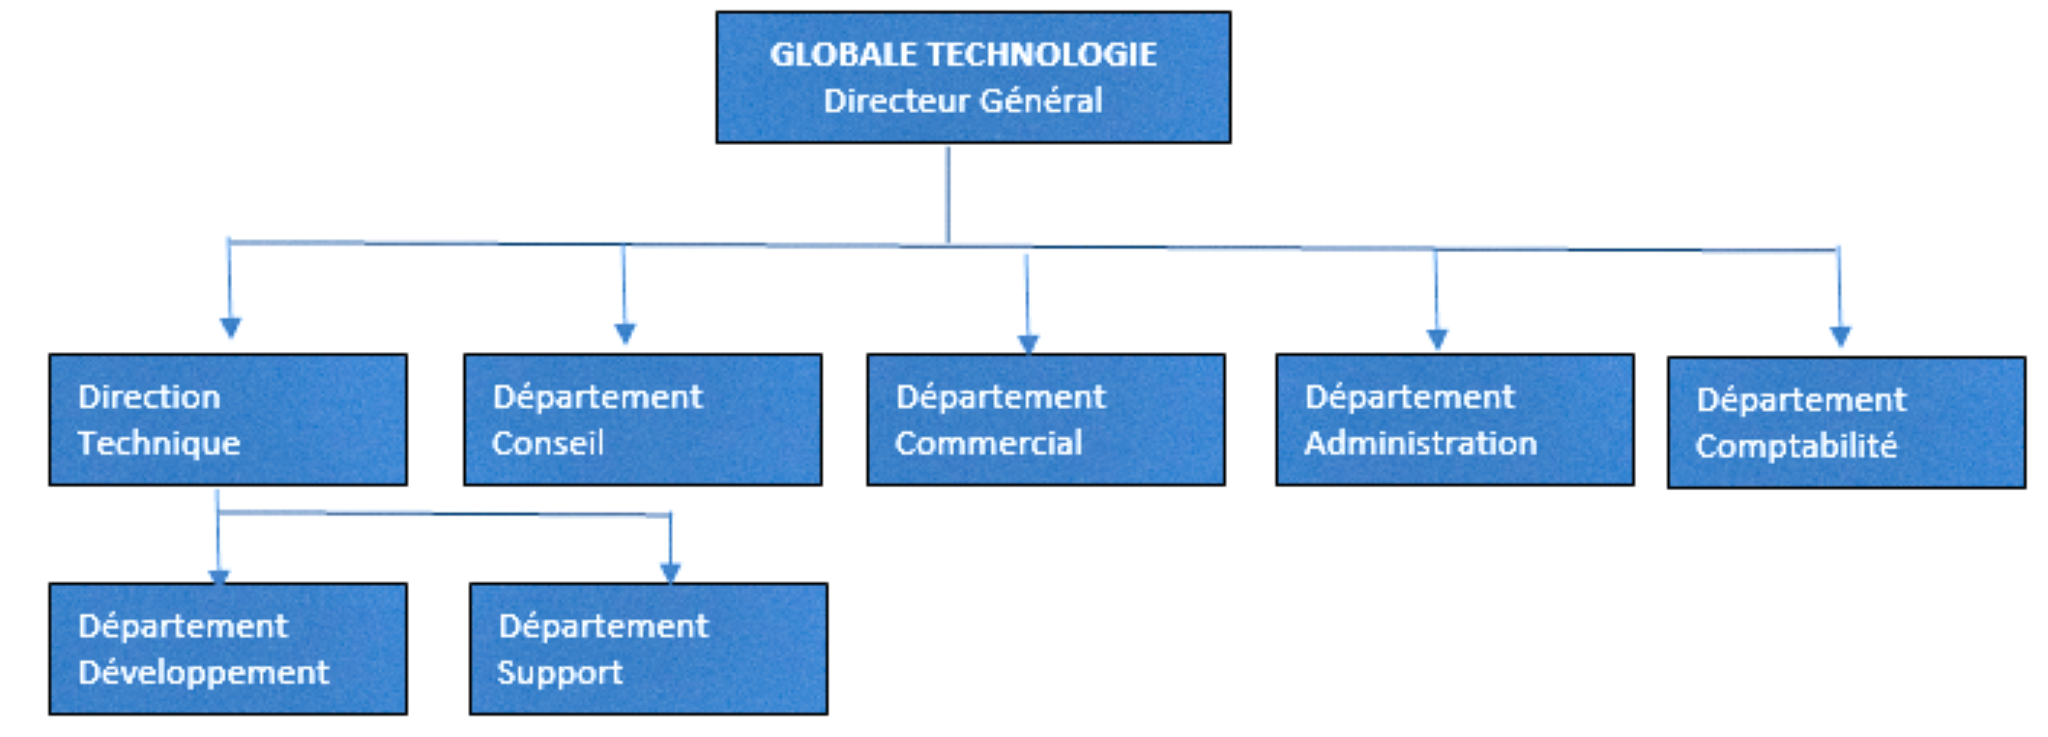
\includegraphics{img/organigramme}
	\caption{Organigramme De Globale Technologies}
	\label{Tux}
\end{figure}
\subsection{Présentation de la Societe Gtech}

\subsection{Domaines d'activités}
\noindent Les nouvelles technologies et l’informatique ont investi tous les domaines d’activités de l’entreprise et sont aujourd’hui de véritables instruments de pilotage stratégique.
\\
\noindent Globale technologies répond à un besoin d’accompagnement technique des entreprises face aux enjeux du système numérique. Surveiller, analyser, rapporter, conseiller, former, maintenir. 
\\
\noindent L’activité de Globale technologies est particulièrement hétérogène.
De manière générale, deux types de prestations sont proposés, à savoir la régie et le forfait. Pour le premier cas, Globale Technologies dépêche les ressources humaines afin de réaliser le contrat dans les locaux de l’entreprise cliente. En revanche, une prestation forfaitaire implique des prestations en externe, avec ses propres ressources matérielles et humaines. En raison de la complexité des tâches, des compétences techniques avérées (réseaux et télécoms, informatique industrielle, etc.) couplées à une connaissance globale des secteurs d’activité sont nécessaires pour mener à bien notre mission.

\section{Présentation du sujet}
\noindent Notre travail est de mettre en place Un registrar, ou bureau d'enregistrement qui est une société spécialise dans l'enregistrement et la réservation de noms de domaine.
\\
\noindent
Dans le monde d'Internet, les noms de domaine, en particulier ceux de premier niveau comme le .com, ne peuvent être achetés ou vendus. Ils font l'objet d'une location pour une durée déterminée et les sites web qui souhaitent l'exploiter doivent alors s'inscrire auprès d'un registrar.
\\
Nous allons concevoir une plateforme de Réservation et d’enregistrement de nom de domaine qui permettra aux Entreprises et Particuliers de pouvoir se procurer facilement un nom de domaine, Un Hébergement web ou bien même de faire doter leurs site web d’un certificat SSL.
En plus de ça nous allons concevoir une plateforme de virtualisation basée sur les technologies KVM et OPENVZ qui permettra à toutes personnes d’acquérir facilement un Serveur dédié virtuel qui sera conforme aux attentes et exigences du client.

\subsection{Contexte} 
\noindent $\blacktriangleright$ La Révolution Internet
\\
\noindent En moins de dix ans, l’internet a bouleversé la vie quotidienne et la gestion des entreprises, a transformé les relations économiques et sociales, a modifié les rapports entre les pays et les hommes, il est devenu le média qui a connu la plus forte croissance de l’histoire de tous les moyens de communication., il ne s’inscrit pas dans une simple logique de diffusion puisqu’il permet de recevoir mais aussi d’émettre. Cette particularité que l’on appelle l’interactivité est unique dans le monde des médias. Elle a profondément modifié les modes de communication entre les individus et a permis de créer de nouveaux liens sociaux, de susciter de nouveaux comportements, de mettre en place des communautés particulières. Au sein des entreprises, l’interactivité a aussi transformé la manière de communiquer avec le marché. À la communication unidirectionnelle s’est substituée avec Internet une communication bidirectionnelle : les internautes reçoivent certes des informations mais en fournissent aussi.  
\\
\\
\noindent $\blacktriangleright$ Les Sites internet de nos jours
\\
\noindent Il est aujourd’hui très important d’avoir un site internet pour une entreprise. Afin d’être présent sur le web, pour notamment accroitre sa clientèle en touchant un large public. L’avantage d’un site internet est qu’il est accessible tout le temps et permet une communication libre pour un faible cout annuel. Que ce soit pour présenter une activité, parler de ses produits, faciliter la communication avec des partenaires ou répondre aux questions habituelles des clients, le site internet est l’outil idéal à ne pas négliger
\\
\\
$\blacktriangleright$ \noindent La virtualisation des serveurs    
\\
\noindent La virtualisation est aujourd’hui une composante légitime des parcs technologiques organisationnels. La virtualisation a progressé de façon indéniable dans les organisations au cours des dernières années. La plupart des grandes organisations, la majorité des moyennes entreprises et un nombre croissant de petites entreprises ont recours à la virtualisation.                                            La virtualisation a entraîné des changements dans l’offre des fournisseurs de matériel technologique et dans les pratiques d’approvisionnement des organisations.
\subsection{Problématique}
\noindent Le marché des noms de domaine est un marché que les pays africains ont laissé dans un esprit de gestion informel qui échappe à toute logique de sécurisation et de protection des utilisateurs, de moralisation du marché par un encadrement des prix.\\
\noindent En l’absence d’acteurs agréés, le marché des Noms de domaine échappe à toute régulation ou contrôle. Au niveau mondial il obéit à une organisation de type Registry (Registrar), alors qu’en Afrique, l’absence de Registrars rend le marché très informel et soumis à des spéculations de tous genres. Il y a plus de 950 registrars dans le monde entier qui sont les intermédiaires agréés qui ont la responsabilité de rendre les Noms de domaines accessibles aux populations selon une logique contractuelle qui permet de garantir que les règles élémentaires de marché sont respectées, alors qu’en Afrique, on n’en compte que 5 présentement, pour une population proche du milliard d’habitants.  \\                                                            
\noindent La faiblesse des infrastructures de gestion de Noms de domaine Internet dans nos pays engendre des difficultés liées au mode de paiement pour se procurer un site internet 

\subsection{Objectifs}
\noindent Objectif général 
\\
\noindent $\blacktriangleright$ Notre objectif général c’est de réaliser une application une plateforme de Réservation et D’enregistrement de nom de domaine, de virtualisation et d’hébergement web qui permettra aux Entreprises et Particuliers de pouvoir se procurer facilement un nom de domaine, Un Hébergement web, un serveur virtuel ou bien même de faire doter leurs site web d’un certificat SSL.
\\
\noindent Sous Objectifs
\\ $\blacktriangleright$ Augmenter Le Nombre de Registrar en Afrique 
\noindent
\\ $\blacktriangleright$ Faciliter Le mode de paiement
\noindent
\\ $\blacktriangleright$ Avoir un site web a un à un prix accessible
\noindent
\\ $\blacktriangleright$ Avoir un serveur Virtual performant a un prix raisonnable 

\subsection{RESULTATS ATTENDUS}
\noindent Nous souhaitons réaliser une application fonctionnelle qui se déroule convenablement de même que l’ensemble de ses fonctionnalités et facile à utiliser.
De ce fait l’application devra permettre aux Entreprises et Particuliers d’obtenir un nom de domaine facilement de même qu’un hébergement web 
Aussi à travers notre applications les utilisateurs pourrons commander un serveur dédie ou virtuel, des certificats SSL-TLS.
\subsection{DEMARCHE METHODOLOGIQUE}
\noindent Pour la phase d’analyse nous procèderons d’abord par :
\noindent
\\
$\blacktriangleright$ Le recueil des besoins fonctionnels 
\noindent
\\
$\blacktriangleright$ Le recueil des besoins techniques  
\noindent
\\
$\blacktriangleright$ L’illustration du projet par des diagrammes UML :
\\
$\blacktriangleright$ Diagramme de contexte Dynamique
\\
$\blacktriangleright$ Diagramme de cas d’utilisation
\\
$\blacktriangleright$ Fiches de description textuelle
\\
$\blacktriangleright$ Diagramme de séquences de quelques cas
\noindent
\\
$\blacktriangleright$ Diagramme de classes
\\
$\blacktriangleright$ Diagramme de déploiement
\\
$\blacktriangleright$ Pour la phase de conception nous utiliserons :
\\
$\blacktriangleright$ La méthode agile Scrum dédiée à la « gestion de projet »
\\
\begin{figure}[H]
	\centering
	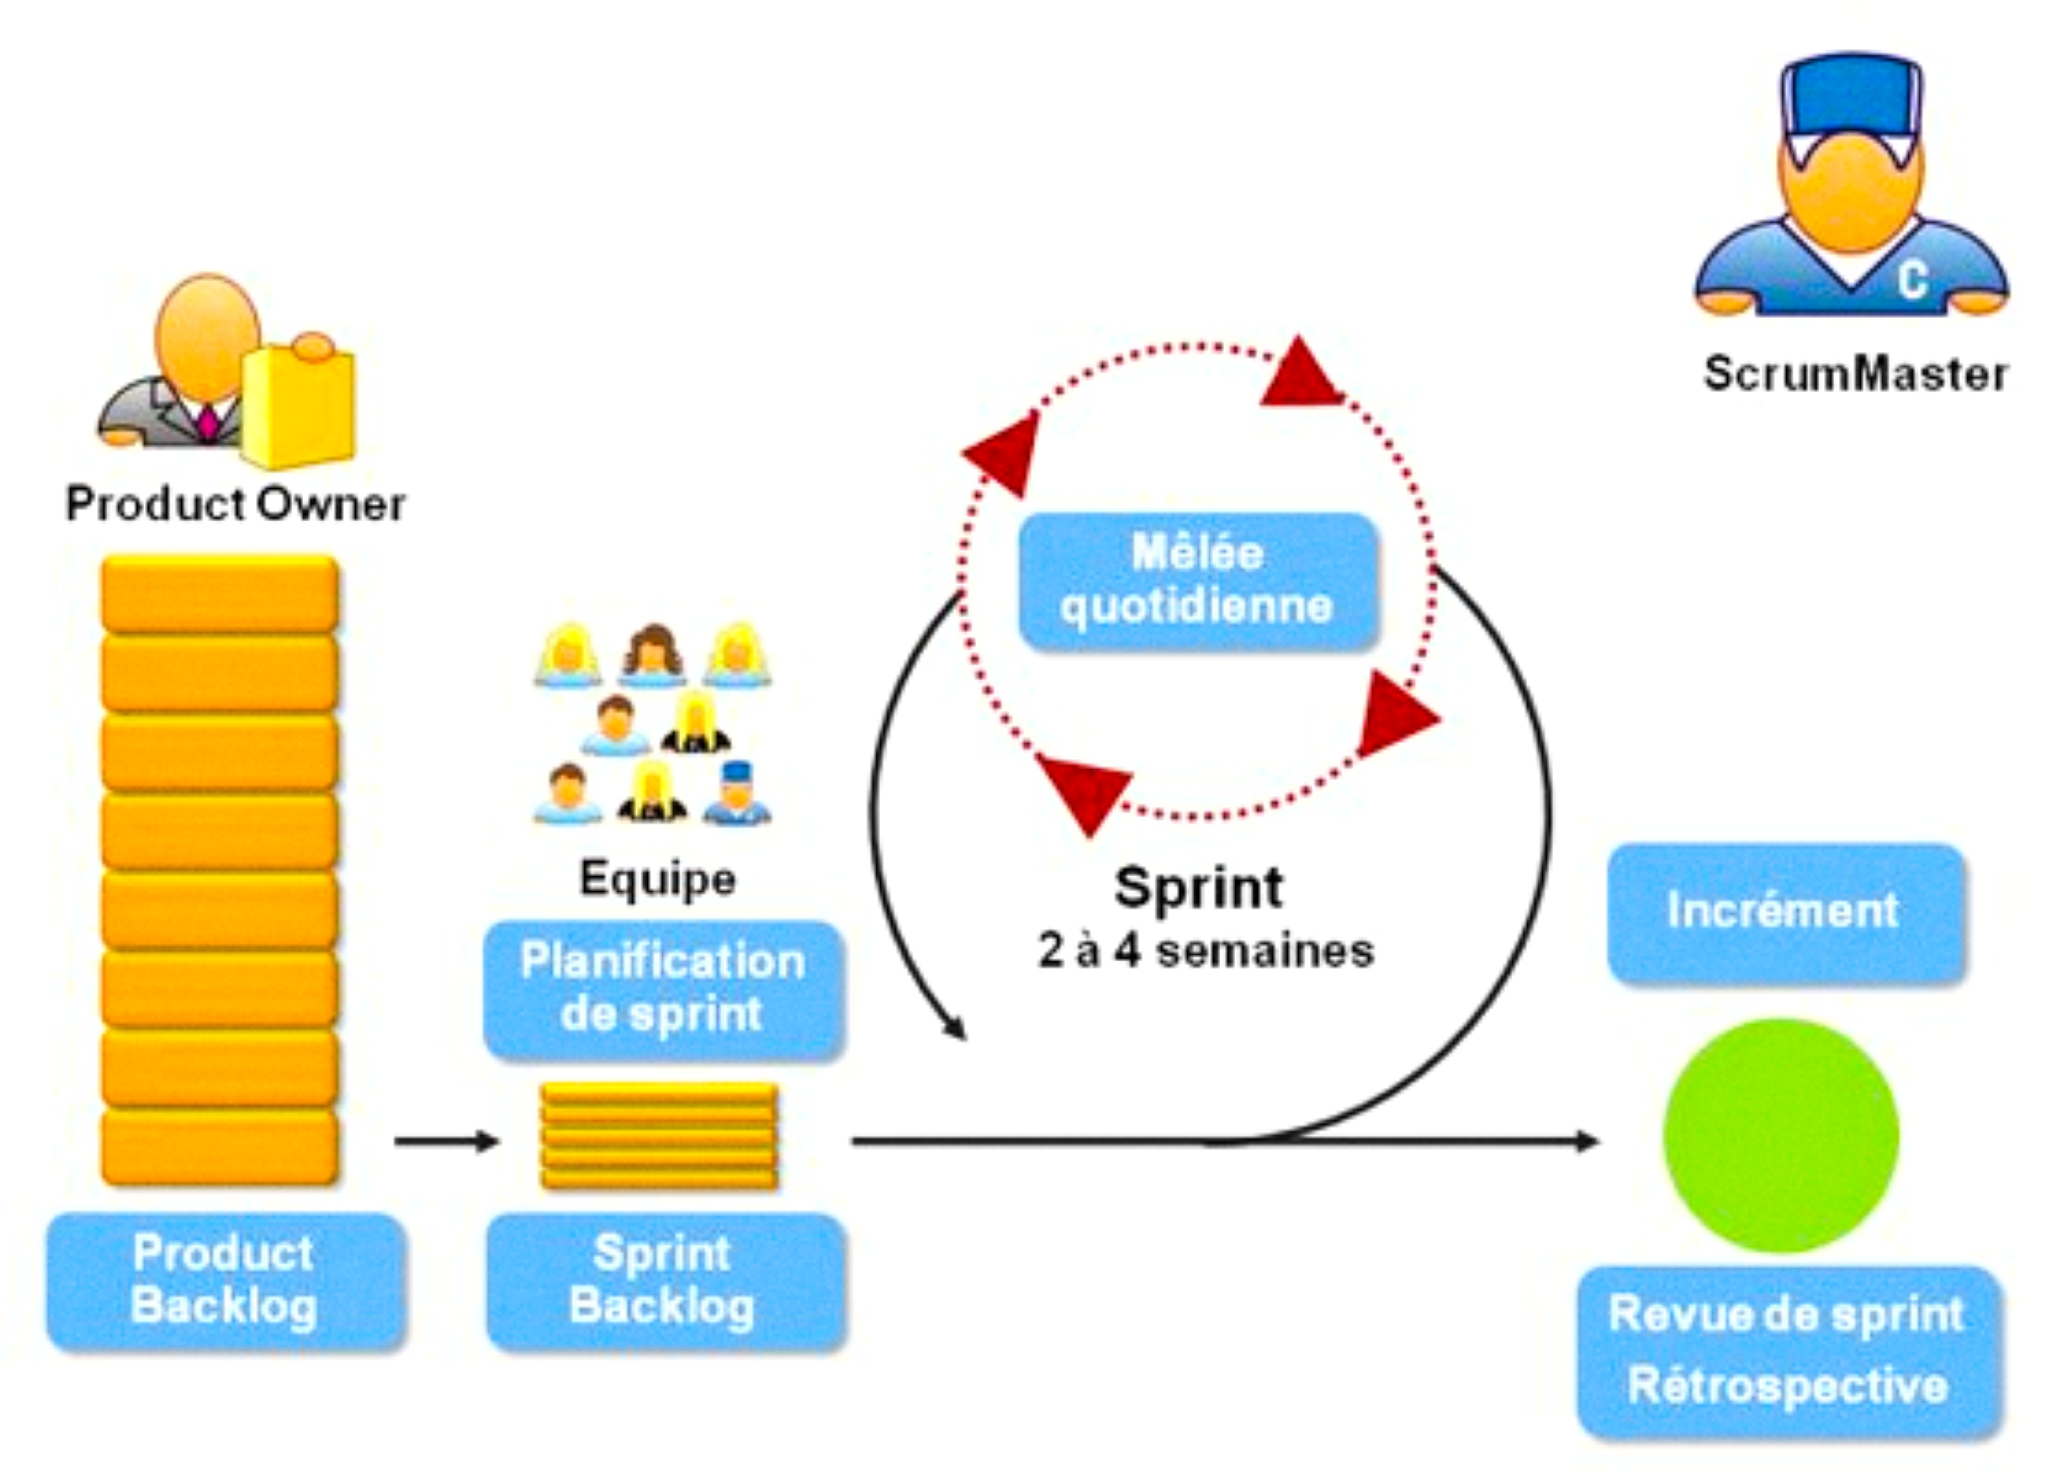
\includegraphics{img/scrumprocess}
	\caption{Le processus Scrum}
	\label{Tux}
\end{figure}
\noindent Le Product Owner qui porte la vision du produit à réaliser et travaille en interaction avec l’équipe de développement. Il s’agit généralement d’un expert du domaine métier du projet. 
L’Equipe de Développement qui est chargée de transformer les besoins exprimés par le Product Owner en fonctionnalités utilisables. Elle est pluridisciplinaire et peut donc encapsuler d’autres rôles tels que développeur, architecte logiciel, DBA, analyste fonctionnel, graphiste/ergonome, ingénieur système. 
Le Scrum Master qui doit maîtriser Scrum et s’assurer que ce dernier est correctement appliqué. Il a donc un rôle de coach à la fois auprès du Product Owner et auprès de l’équipe de développement. Il doit donc faire preuve de pédagogie. Il est également chargé de s’assurer que l’équipe de développement est pleinement productive. Généralement le candidat tout trouvé au rôle de Scrum Master est le chef de projet. Celui-ci devra cependant renoncer au style de management « commander et contrôler » pour adopter un mode de management participatif. 
La vie d’un projet Scrum est rythmée par un ensemble de réunions clairement définies et strictement limitées dans le temps (timeboxing) : 
\\
\noindent
$\blacktriangleright$ Planification du Sprint (Sprint = itération) : au cours de cette réunion, l’équipe de développement sélectionne les éléments prioritaires du « Product Backlog » (liste ordonnancée des exigences fonctionnelles et non fonctionnelles du projet) qu’elle pense pouvoir réaliser au cours du sprint (en accord avec le « Product Owner »). 
\\
\noindent
$\blacktriangleright$ Revue de Sprint : au cours de cette réunion qui a lieu à la fin du sprint, l’équipe de développement présente les fonctionnalités terminées au cours du sprint et recueille les feedbacks du Product Owner et des utilisateurs finaux. C’est également le moment d’anticiper le périmètre des prochains sprints et d’ajuster au besoin la planification de release (nombre de sprints restants). 
\\
\noindent
$\blacktriangleright$ Rétrospective de Sprint : la rétrospective qui a généralement lieu après la revue de sprint est l’occasion de s’améliorer (productivité, qualité, efficacité, conditions de travail, etc.) à la lueur du « vécu » sur le sprint écoulé (principe d’amélioration continue). 
\\
\noindent
$\blacktriangleright$ Mêlée quotidienne : il s’agit d’une réunion de synchronisation de l’équipe de développement qui se fait debout (elle est aussi appelée « stand up meeting ») en 15 minutes maximum au cours de laquelle chacun répond principalement à 3 questions : « Qu’est-ce que j’ai terminé depuis la dernière mêlée ? Qu’est-ce que j’aurai terminé d’ici la prochaine mêlée ? Quels obstacles me retardent ? » 
\\
\noindent
$\blacktriangleright$ Présentation des rôles dans le projet : 
Product owner : 
Globale Technologies une SSII basée à Dakar reconnue comme intégrateur incontournable.
Scrum Master 
Dr Mandicou Ba, enseignant-chercheur, expert en Génie Logiciel
Equipe de développement : 
Babacar Fall, développeur et chef de projet informatique

%CHAPITRE 2
\chapter{Analyse et Conception de la solution}
\noindent \textit{\textbf{Résumé:} }
La phase d’analyse et de conception est la première étape du processus de développement que nous avons adopté. En effet, elle formalise et détaille ce qui a été ébauché au cours de l’étude préliminaire, et permet de gérer l’étude fonctionnelle du système. Elle permet ainsi d’obtenir une idée de ce que va réaliser le système en termes de métier (comportement du système).
Tout au long de ce chapitre nous allons commencer par présenter le langage UML, les spécifications fonctionnelles, l’analyse des besoins et enfin la conception. 

\setcounter{minitocdepth}{1}
\minitoc

\section{Présentation du langage UML (Unified Modeling Language)}
\noindent UML donne une définition sur une approche objet plus formelle et apporte la dimension logique à l’approche objet. Pour concevoir en UML, il faut commencer par prendre de la hauteur par rapport au problème qui est posé et utiliser des concepts abstraits complètement indépendants des langages de programmation pour modéliser l’objet. L’utilisation d’un langage de programmation comme support de conception revient à faire une analyse peu précise et réductrice par rapport à une modélisation objet. Et justement à l’inverse de la plupart des technologies objets, UML permet de s’affranchir totalement de tout langage de programmation (permettant ainsi l’écueil de la limitation en vue du langage de programmation) pour élaborer et exprimer des modelés objets. Il a été pensé comme support d’analyse objet.
De plus, UML est un méta modèle : il décrit très précisément tous les éléments de modélisation (permettant ainsi de limiter les ambigüités) et normalise les concepts objets. Étant un méta modèle, UML est valable pour tous les langages de programmation.
Les critères ou les qualités d’UML sont les suivants :
\\
\noindent $\blacktriangleright$ Langage sans ambigüité 
\\
\noindent $\blacktriangleright$ Langage universel
\\
\noindent $\blacktriangleright$ Moyen de définir les structures de programmation
\\
\noindent $\blacktriangleright$ Représentation universelle (communication performante)    
\\  
\noindent $\blacktriangleright$ Notation graphique simple (compréhensible de tout le monde, pas seulement les  
informaticiens).                                                                                                                                             
Modélisation du méta modèle, cette notation graphique est le support du langage UML. Ceci lui permet donc d’être visuellement plus compréhensible (pour comparer ou évaluer) et limite ainsi les ambigüités. UML offre un cadre avec différentes vues complémentaires du système sur plusieurs niveaux d’abstraction, les diagrammes, et contrôle ainsi la complexité dans l’expression des objets.     

\section{SPECIFICATIONS FONCTIONNELLES}
\noindent C’est la représentation des fonctionnalités d’un système du point de vue utilisateur.
Le diagramme de cas d’utilisation est la première étape UML d’analyse d’un système. C’est un moyen simple et facilement compréhensible pour exprimer les besoins des utilisateurs. Il permet de recenser les grandes fonctionnalités d’un système.
Ainsi un cas d’utilisation est une suite d’actions interruptibles exécutées par un acteur sur un système et qui produit un résultat observable pour l’acteur.
\begin{figure}[H]
	\centering
	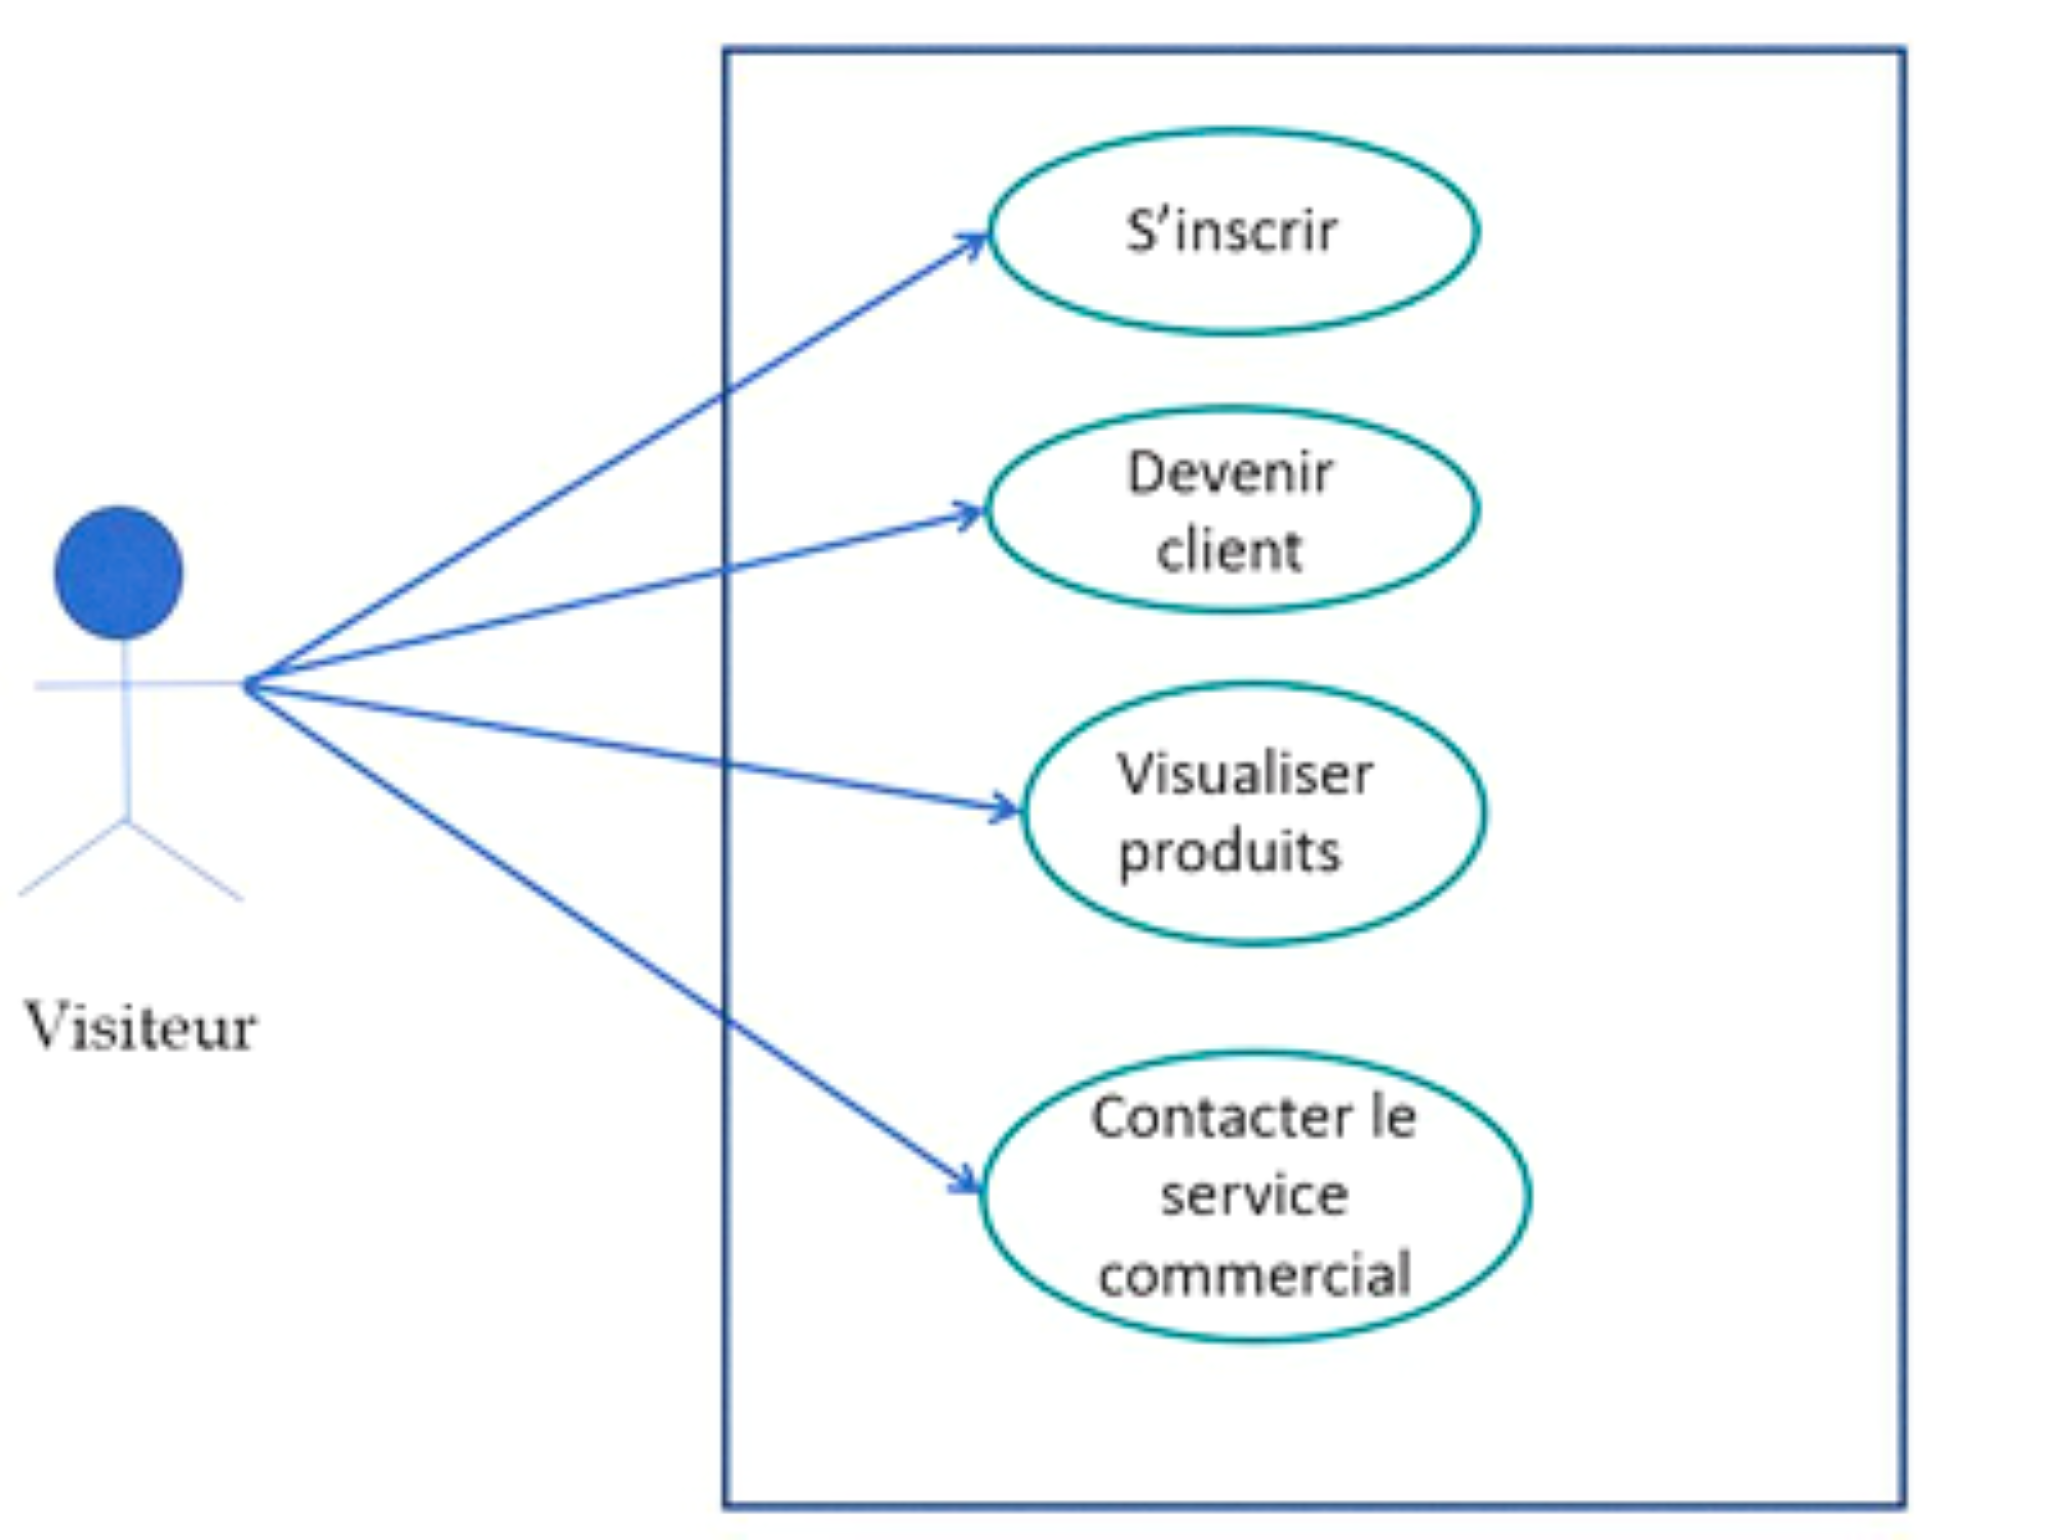
\includegraphics{img/cas-visiteur}
	\caption{Diagramme de Cas d’utilisation de l’acteur Visiteur}
	\label{Tux}
\end{figure}
\begin{figure}[H]
	\centering
	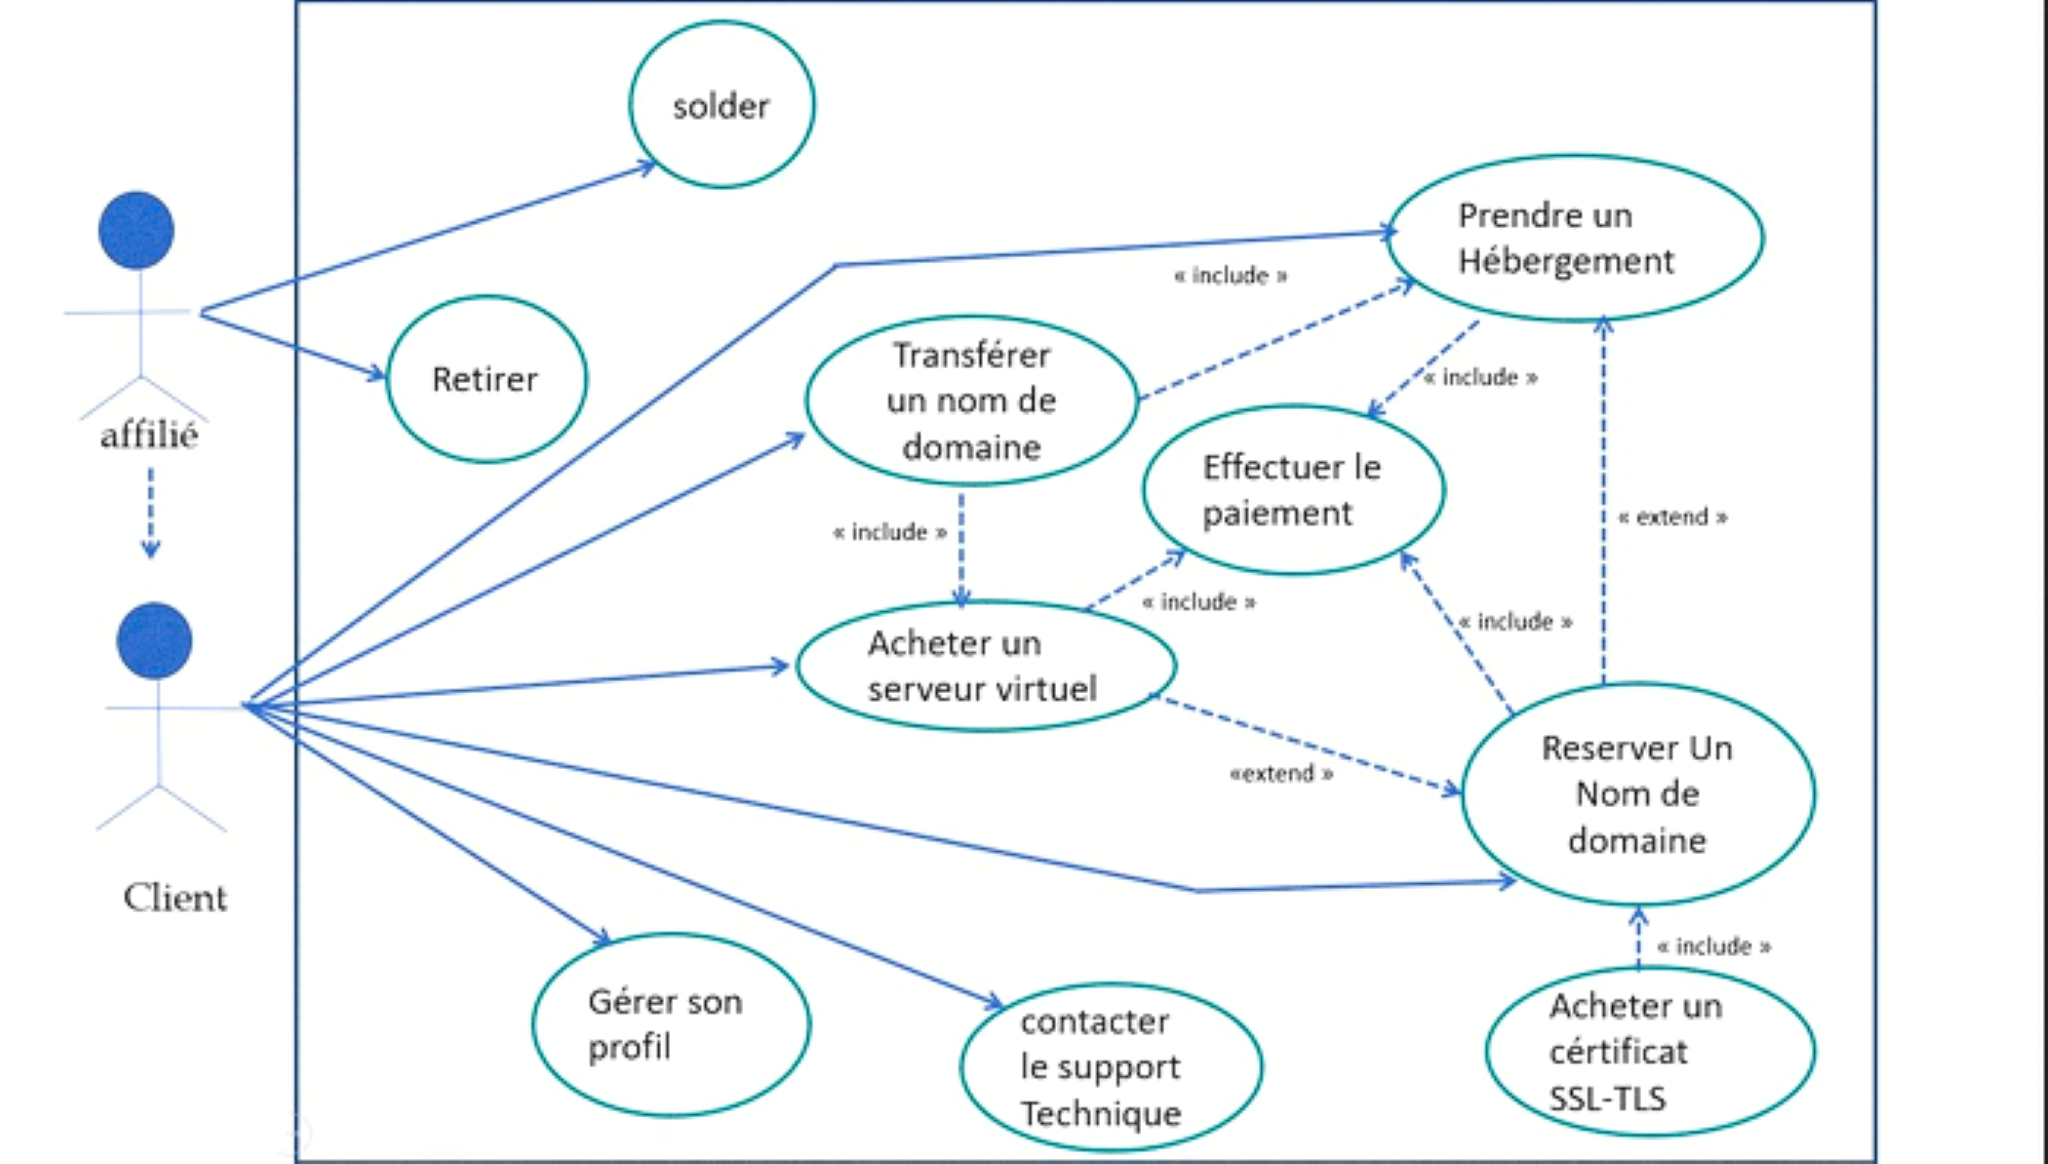
\includegraphics{img/cas-client}
	\caption{Diagramme de Cas d’utilisation de l’acteur client}
	\label{Tux}
\end{figure}
\begin{figure}[H]
	\centering
	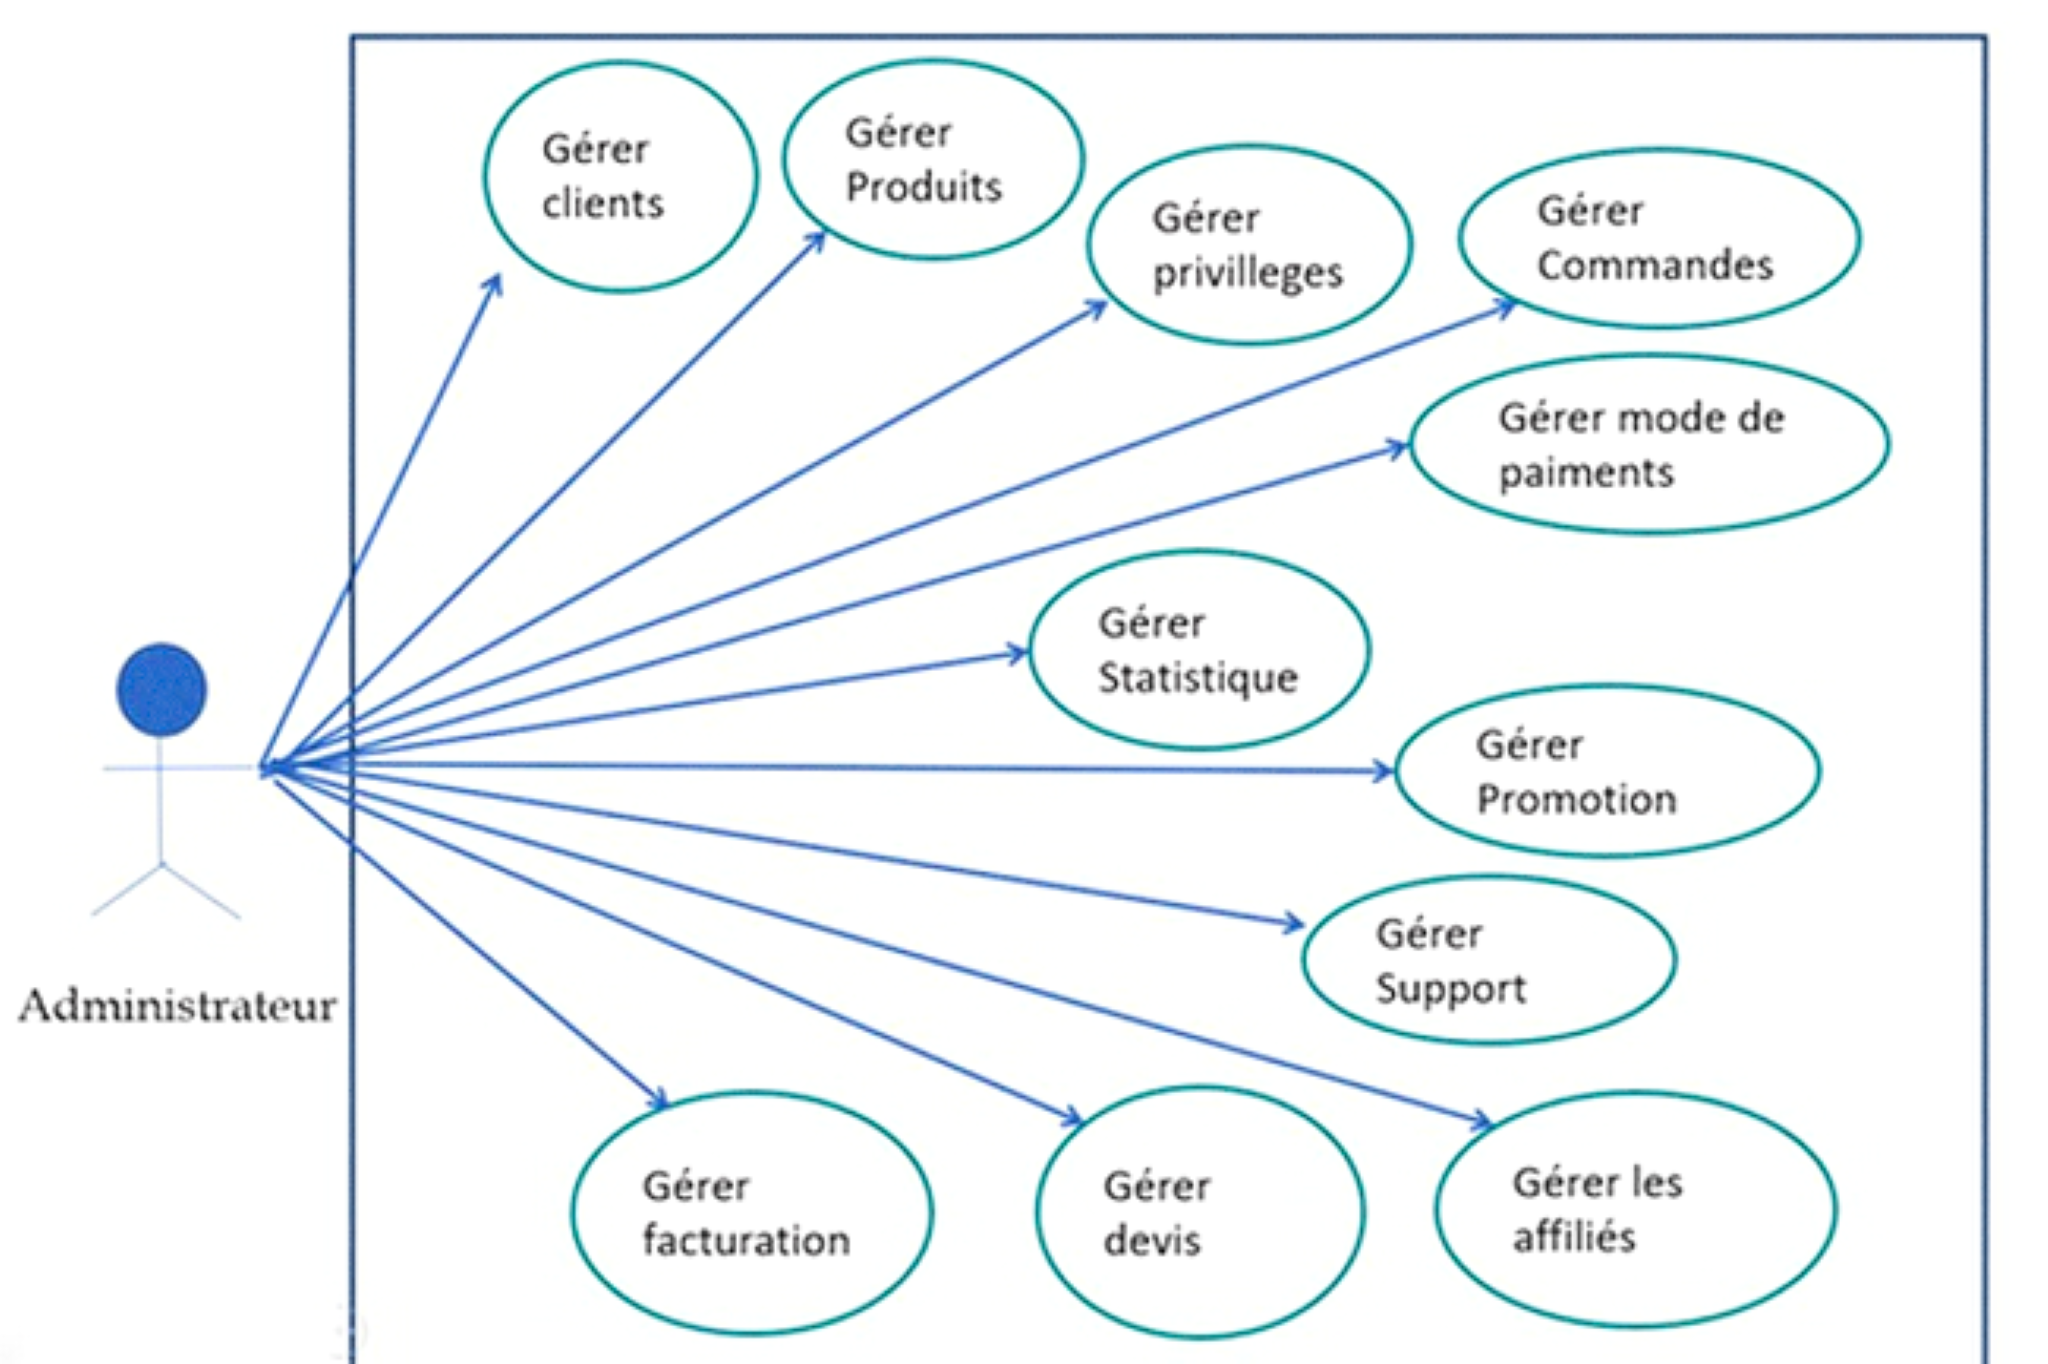
\includegraphics{img/cas-admin}
	\caption{Diagramme de Cas d’utilisation de l’acteur Administrateur}
	\label{Tux}
\end{figure}
\begin{figure}[H]
	\centering
	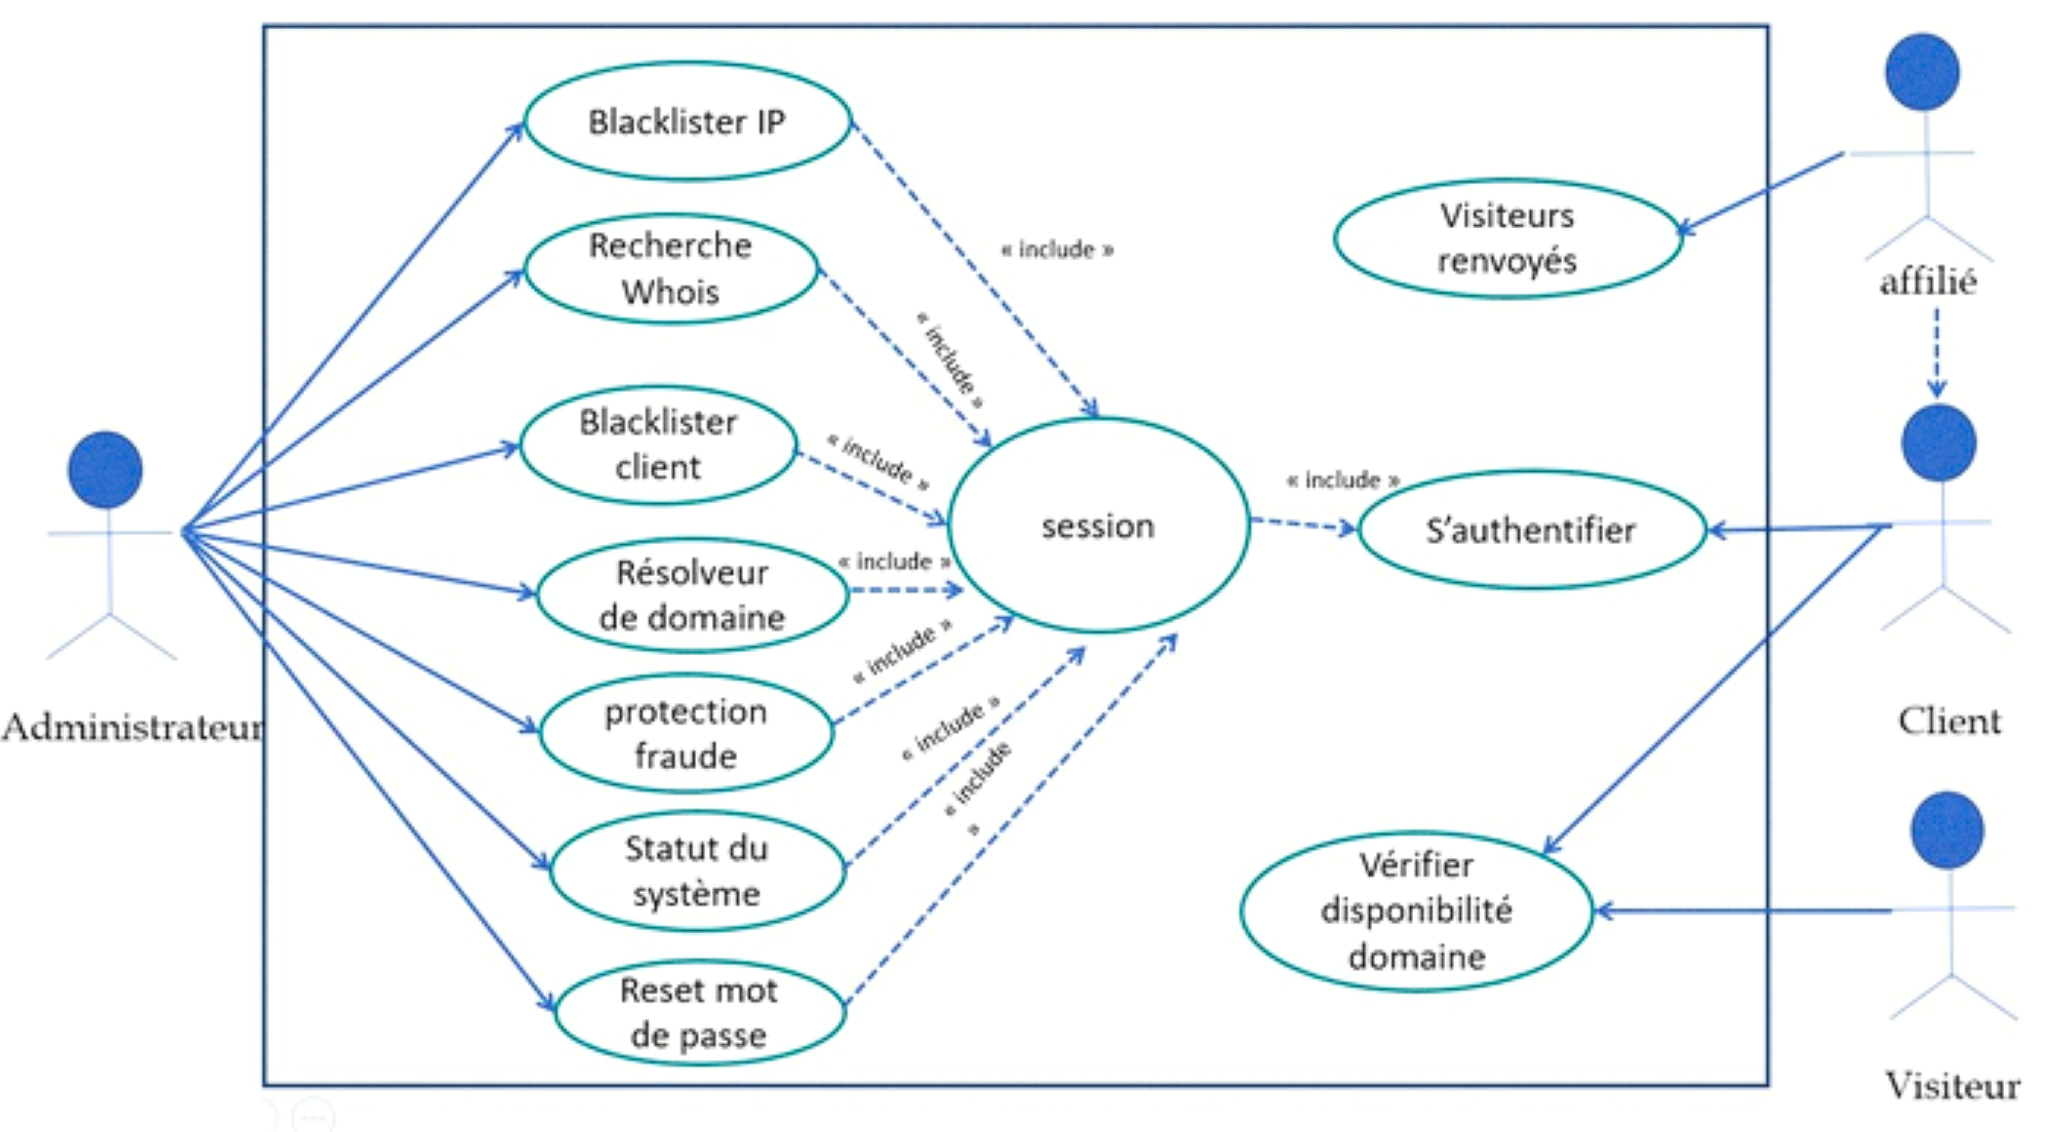
\includegraphics{img/cas-technique}
	\caption{Diagramme de Cas d’utilisationCas des fonctionnalités technique}
	\label{Tux}
\end{figure}
                
\noindent Explication détaillée des cas d’utilisation
\\
\noindent
L’étude de cas d’utilisation a pour objectif de déterminer ce que chaque utilisateur attend du système. La détermination du besoin est basée sur la représentation de l’interaction entre l’acteur et le système.

\noindent $\blacktriangleright$ Authentification : permet d’identifier chaque utilisateur, et de lui donner l’accès aux fonctionnalités propices.

\noindent $\blacktriangleright$ Gérer les commandes : permet aux administrateurs du système de pouvoir ajouter, valider, modifier ou consulter une commande. 

\noindent $\blacktriangleright$ Gérer les Produits : permet aux administrateurs de pouvoir ajouter, supprimer, modifier ou consulter un produit. Il leur permet aussi d’afficher tous les produits existants. 

\noindent $\blacktriangleright$ Gérer les clients : permet aux administrateurs de pouvoir ajouter, supprimer, modifier ou consulter un client. Il leur permet aussi d’afficher tous les clients existants.

\noindent $\blacktriangleright$ Gérer les paiements : permet aux administrateurs de pouvoir ajouter, supprimer, modifier ou consulter un mode de paiement. Il leur permet aussi d’afficher toutes les modes de paiement existants.

\noindent $\blacktriangleright$ Visualiser facture : permet aux administrateurs de pouvoir visualiser les factures générées par le système 

\noindent $\blacktriangleright$ Répondre aux messages : permet aux administrateurs de pouvoir répondre aux messages envoyés par les clients

\noindent $\blacktriangleright$ Gérer son profil : permet aux clients de pouvoir consulter ou modifier facilement son profil

\noindent $\blacktriangleright$ Contacter support : permet aux clients de pouvoir contacter le support technique afin de résoudre un problème 

\noindent $\blacktriangleright$ Réserver un nom de domaine : permet à un client de pouvoir se procurer facilement un nom de domaine 

\noindent $\blacktriangleright$ Transférer un nom de domaine : permet à un client de pouvoir transférer un nom de domaine dans nos serveurs.


\noindent $\blacktriangleright$ Commander un certificat SSL-TLS : permet à un client de pouvoir faire doter son site web d’un certificat SSL-TLS.

\noindent $\blacktriangleright$ Commander un serveur dédié : permet à un client de pouvoir commander un serveur dédie serveur VPS (virtual private server) ou serveur RDP (remote desktop Protocol).

\noindent $\blacktriangleright$ Blacklister une adresse IP : permet à un administrateur de pouvoir interdire une adresse IP ou un ensemble d’adresse IP du système.


\noindent $\blacktriangleright$ Blacklister un client : permet à un administrateur de pouvoir bannir un client du système suite à une violation des conditions d’utilisation.

\noindent $\blacktriangleright$ Modifier son mot de passe en cas de perte : permet à un client de pouvoir réinitialiser son mot de passe en cas de perte.

\section{Fiches Textuelles}
\begin{table}[H]
	\centering
	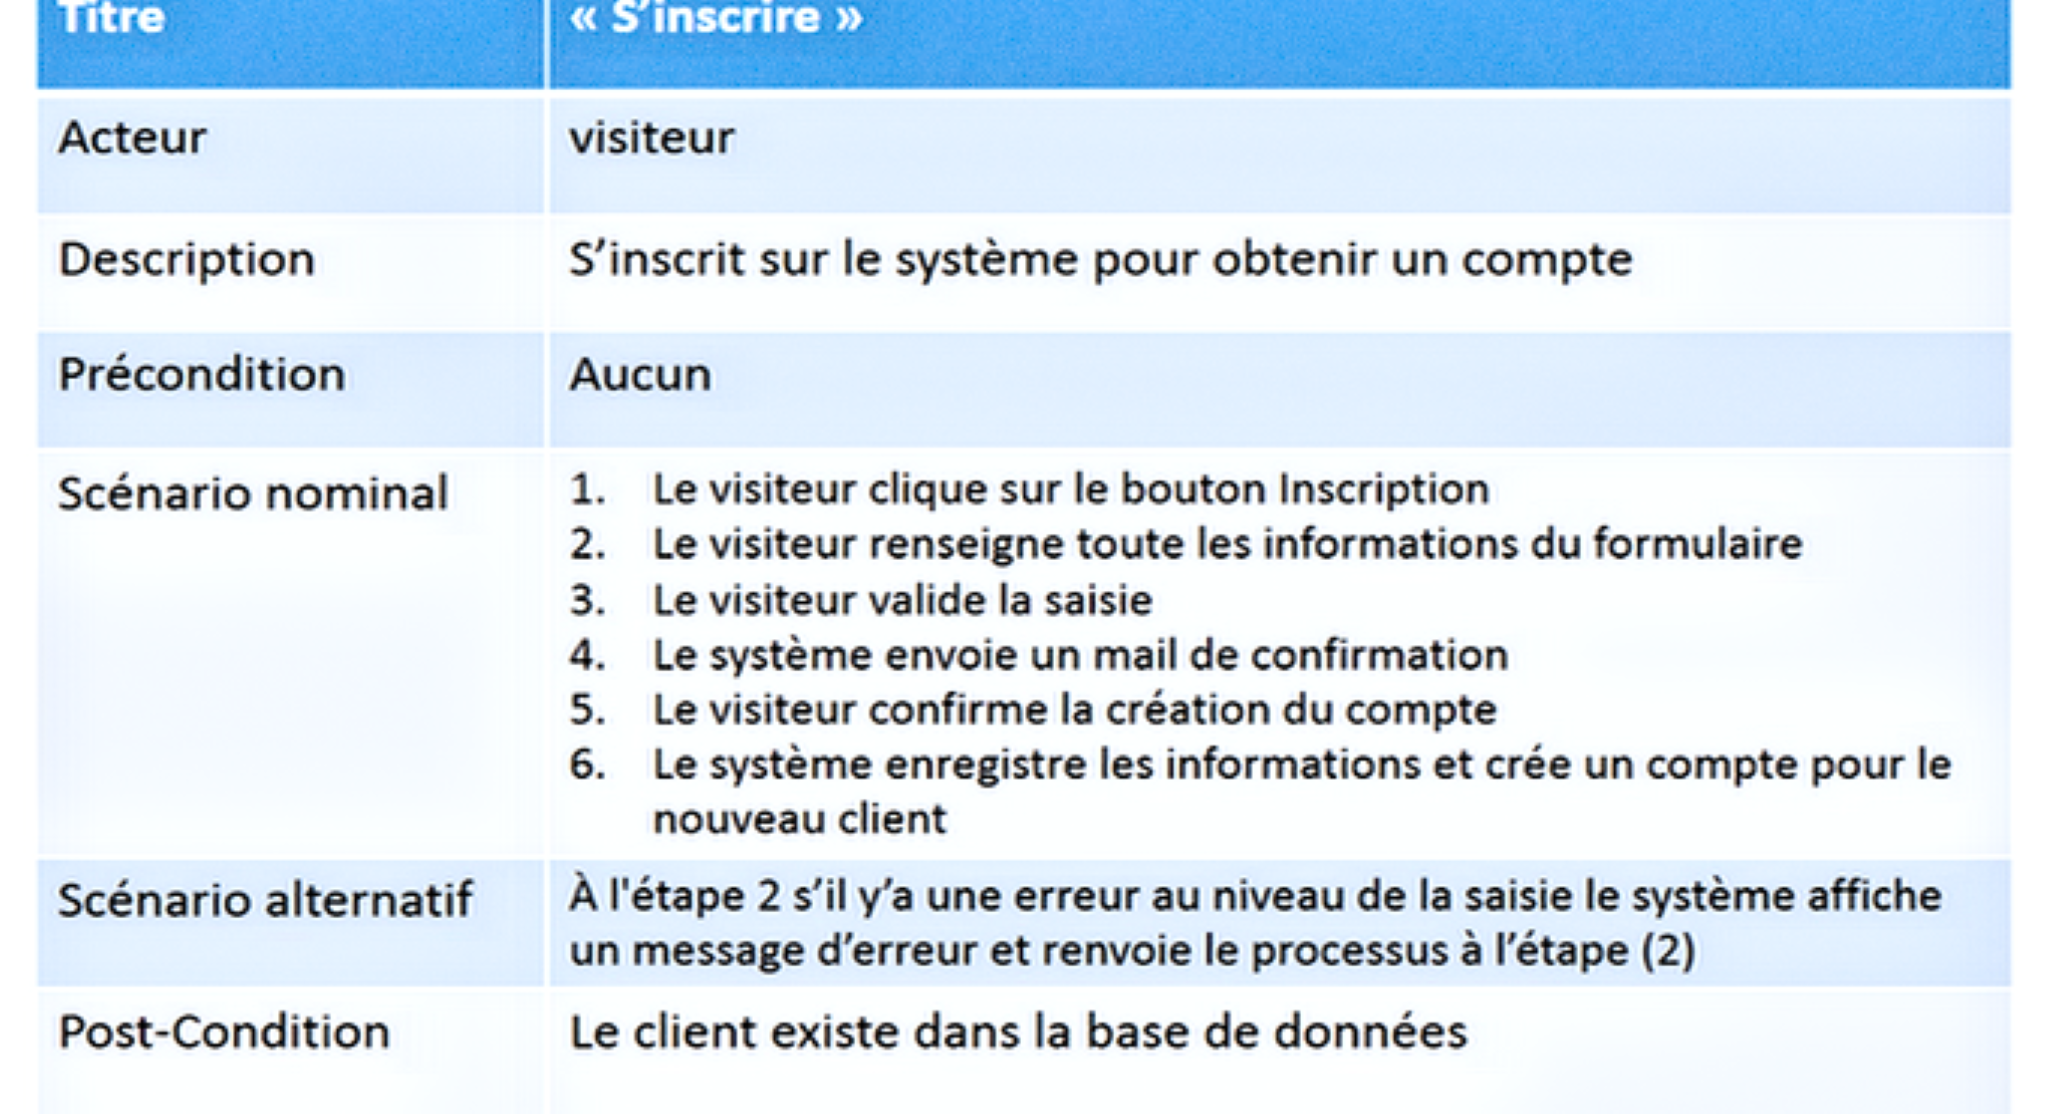
\includegraphics{img/fiche/1}
	\caption{Fiche Textuelle du cas "s’inscrire}
	\label{Tux}
\end{table}
\begin{table}[H]
	\centering
	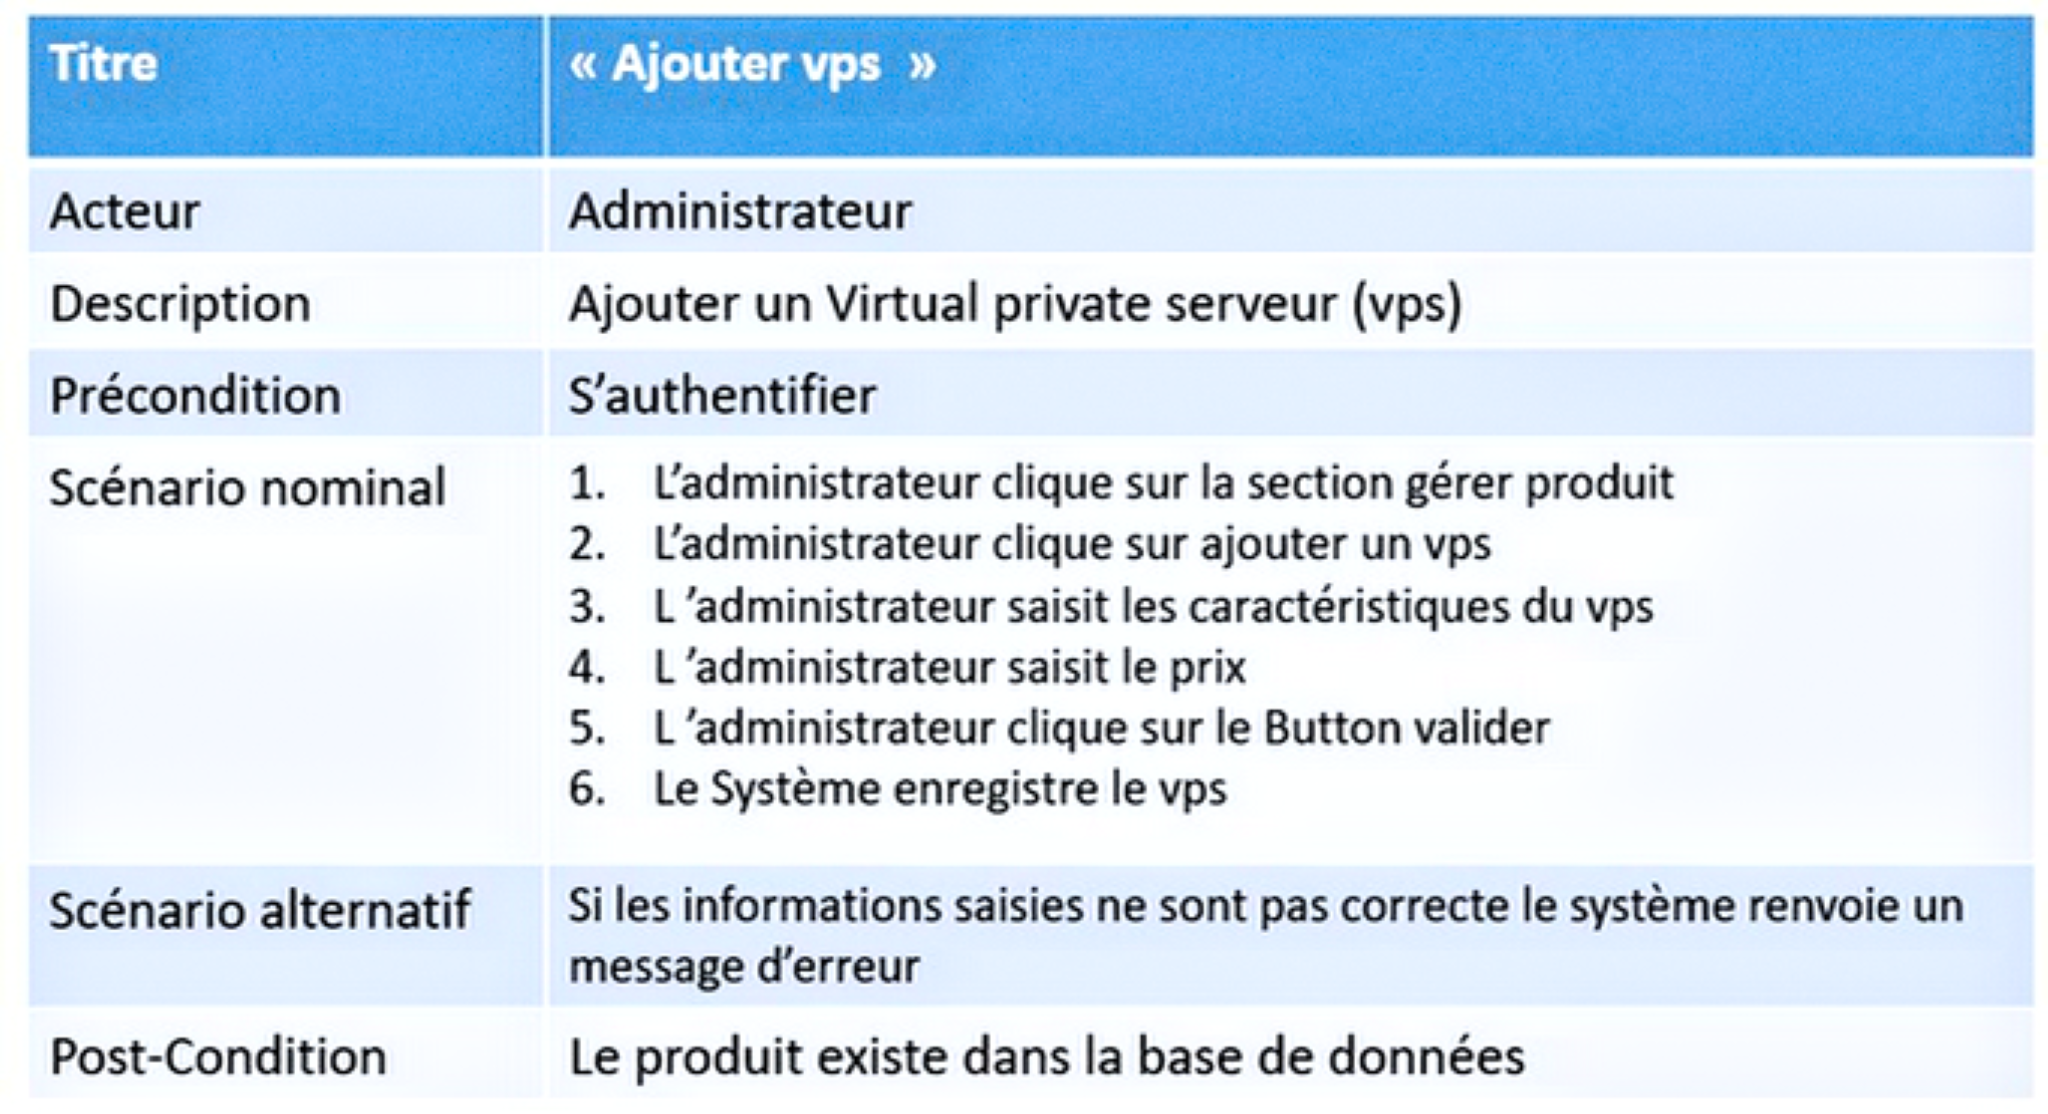
\includegraphics{img/fiche/2}
	\caption{Fiche Textuelle Ajouter VPS}
	\label{Tux}
\end{table}
\begin{table}[H]
	\centering
	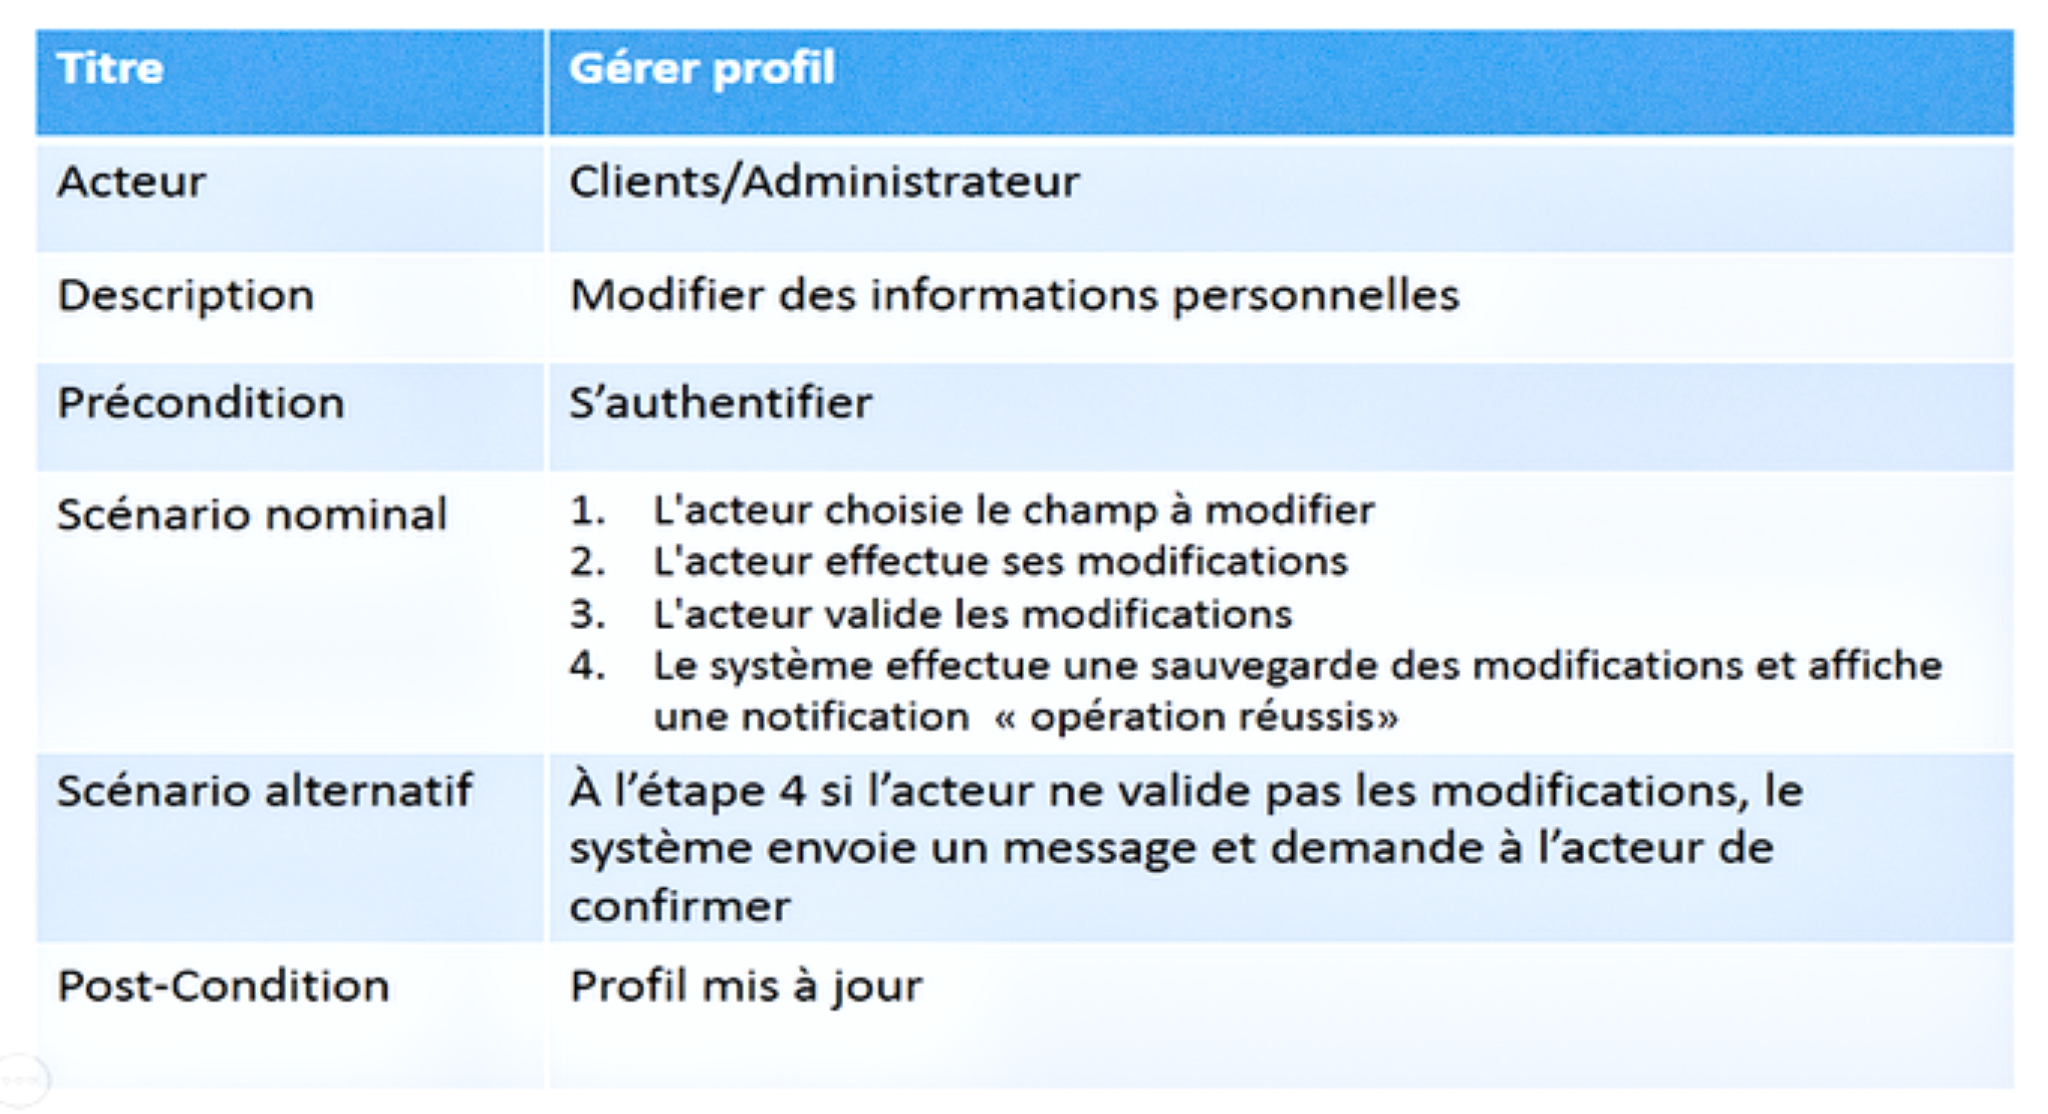
\includegraphics{img/fiche/3}
	\caption{Fiche textuelle du cas "Gérer Profil"}
	\label{Tux}
\end{table}
\begin{table}[H]
	\centering
	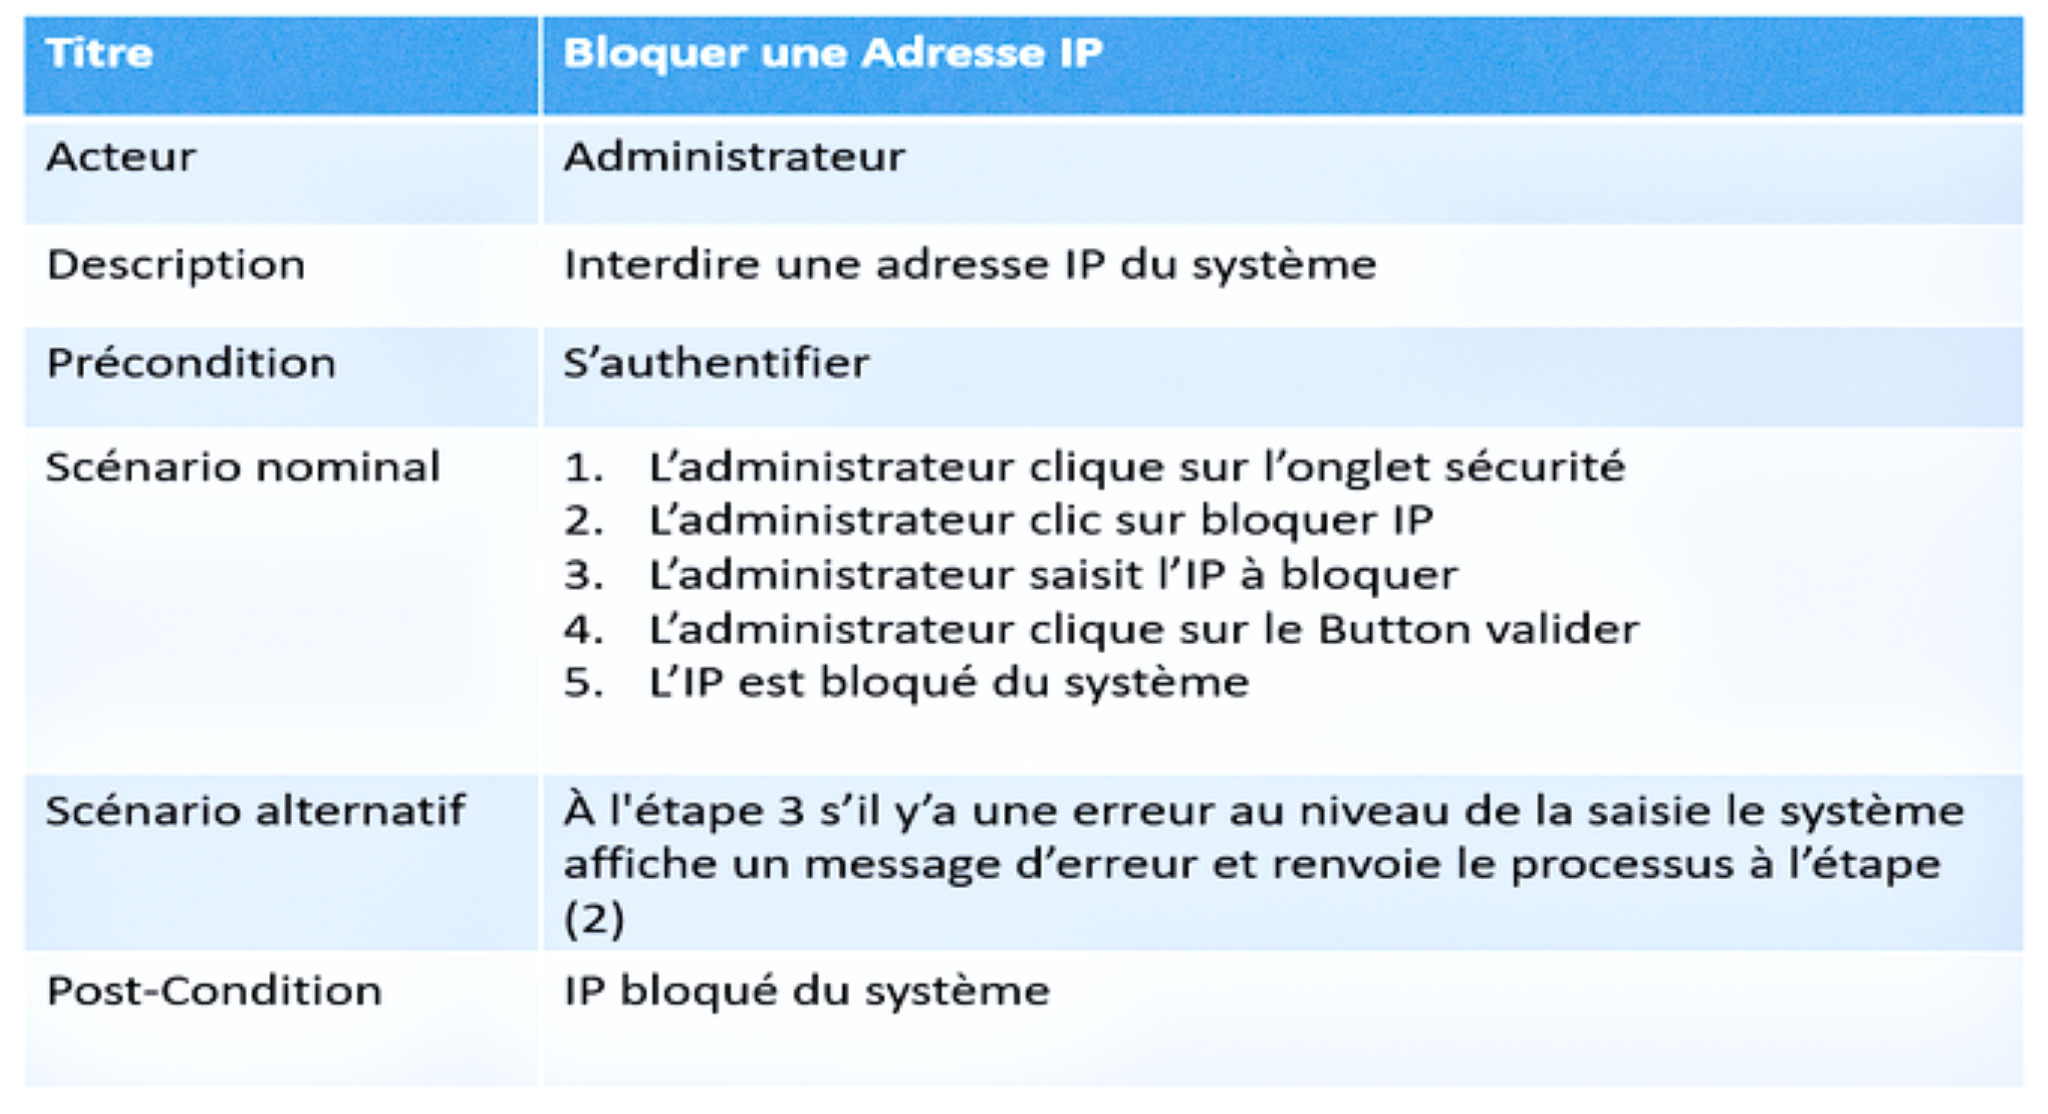
\includegraphics{img/fiche/4}
	\caption{Fiche textuelle du cas "Bloquer une adresse IP"}
	\label{Tux}
\end{table}
\begin{table}[H]
	\centering
	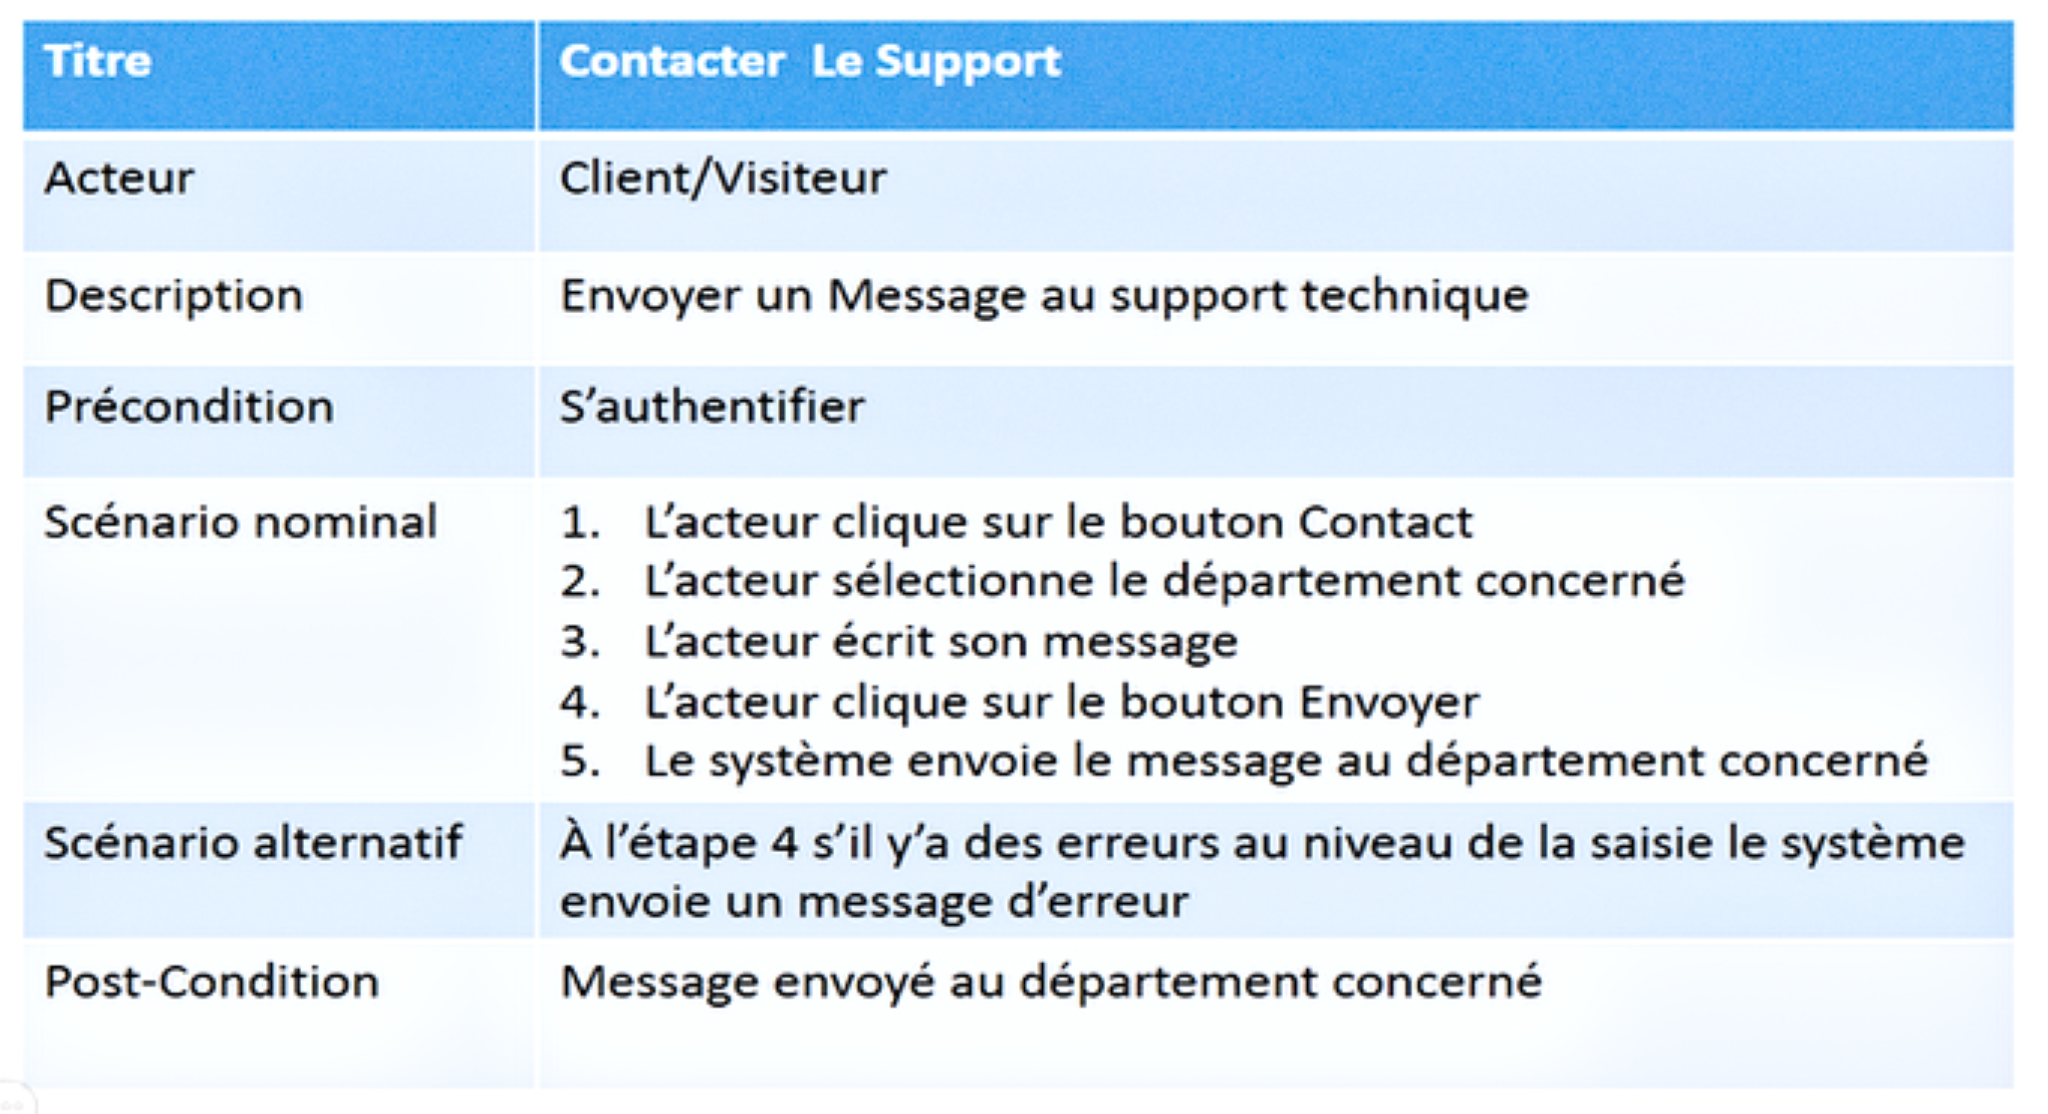
\includegraphics{img/fiche/5}
	\caption{Fiche textuelle du cas "Contacter le support"}
	\label{Tux}
\end{table}
\begin{table}[H]
	\centering
	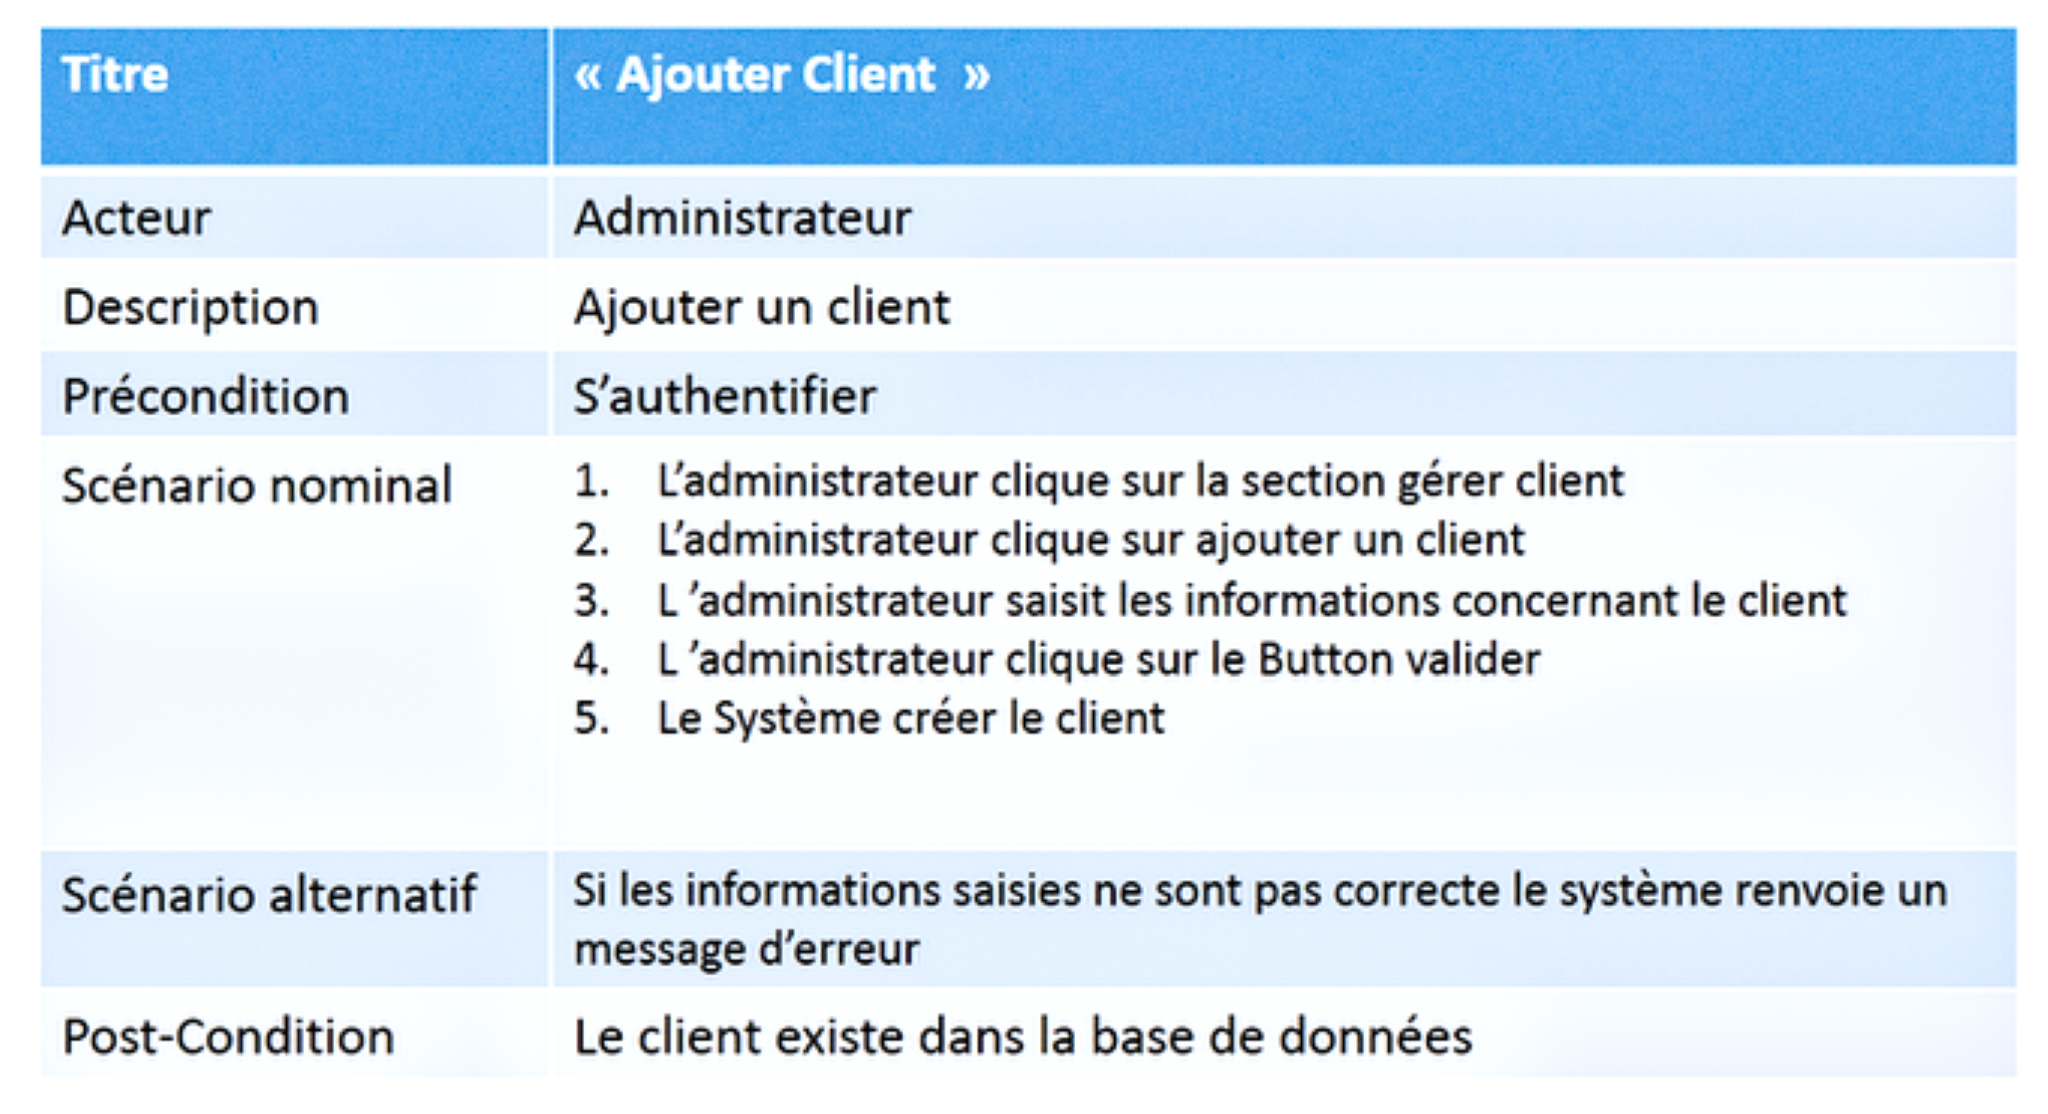
\includegraphics{img/fiche/6}
	\caption{Fiche textuelle du cas "Ajouter Client"}
	\label{Tux}
\end{table}
\begin{table}[H]
	\centering
	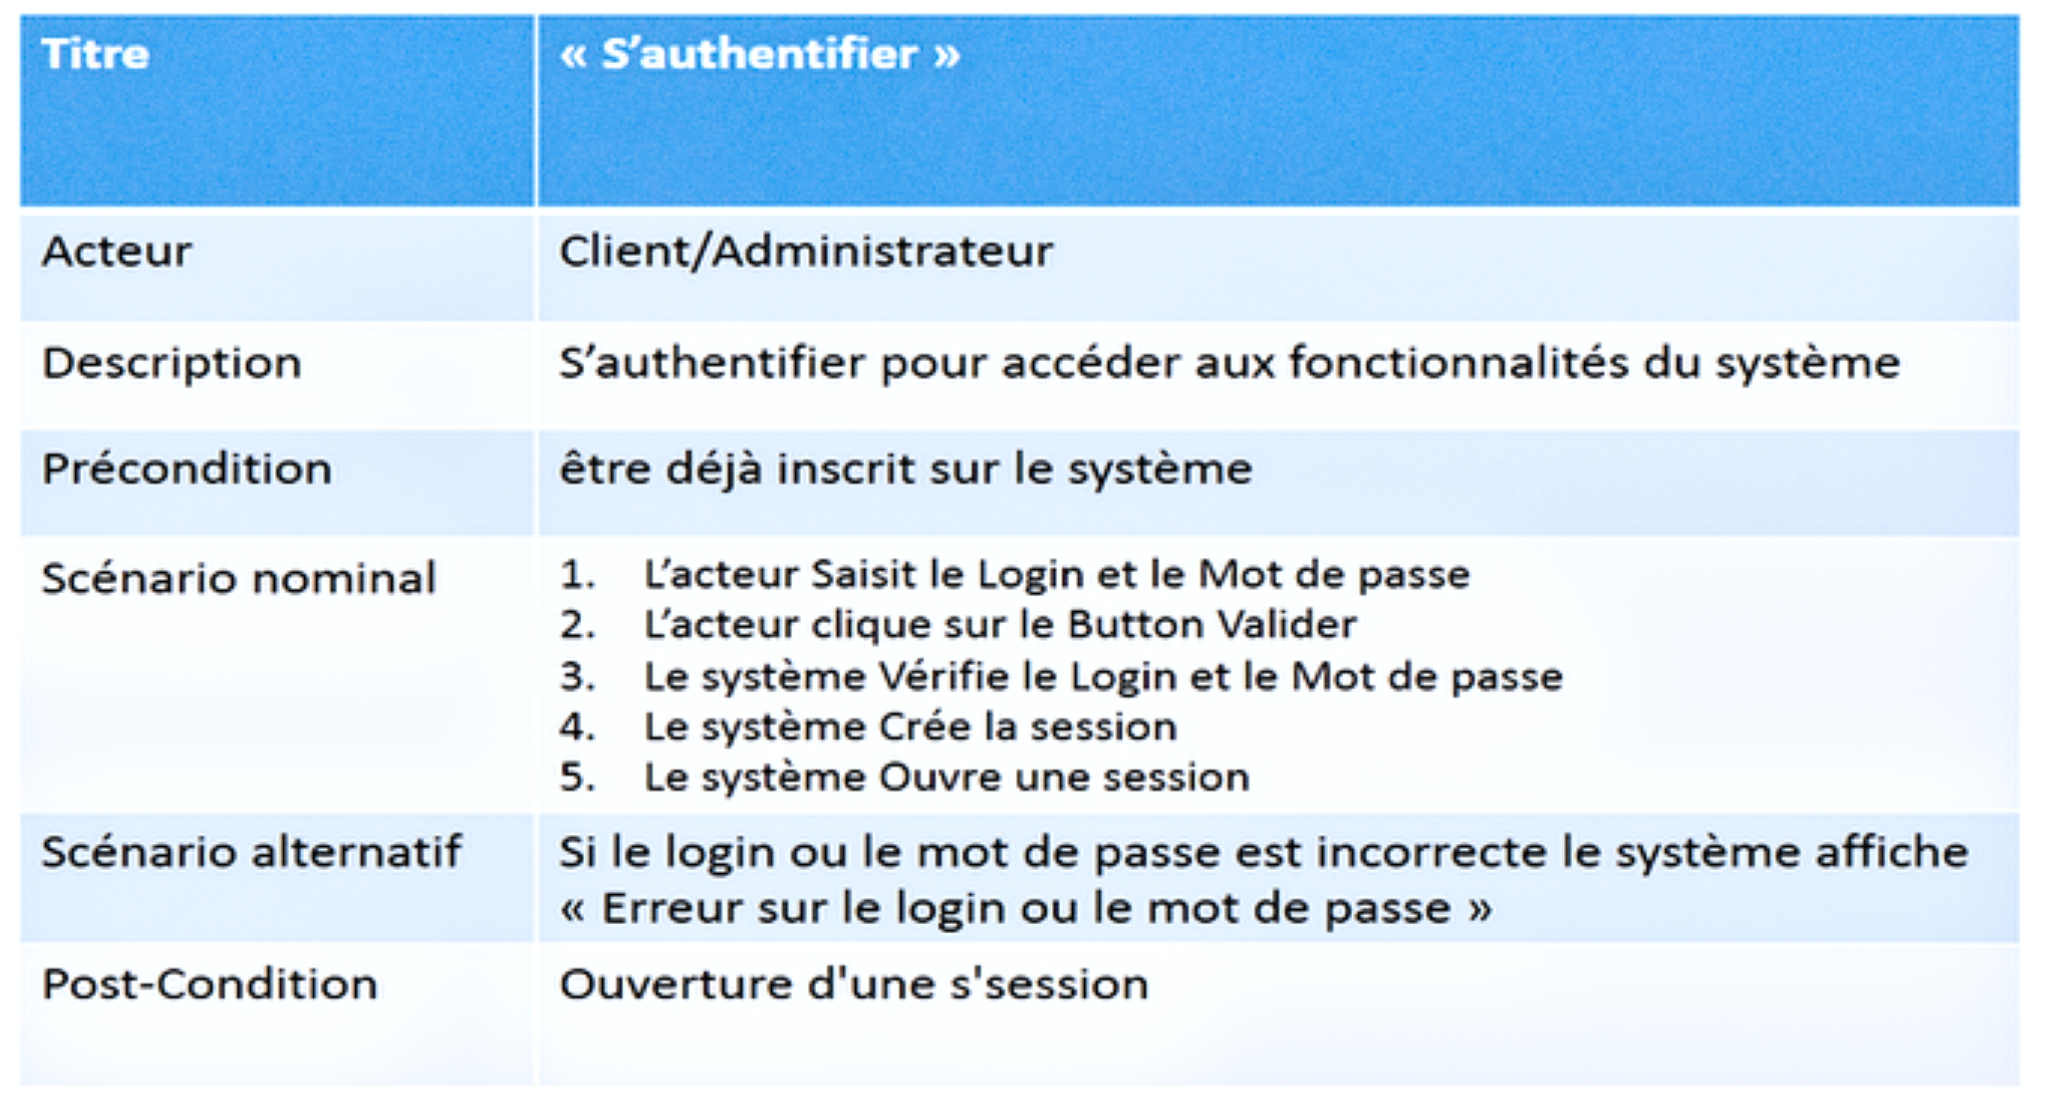
\includegraphics{img/fiche/7}
	\caption{Fiche Textuelle du cas "S’authentifier"}
	\label{Tux}
\end{table}
\begin{table}[H]
	\centering
	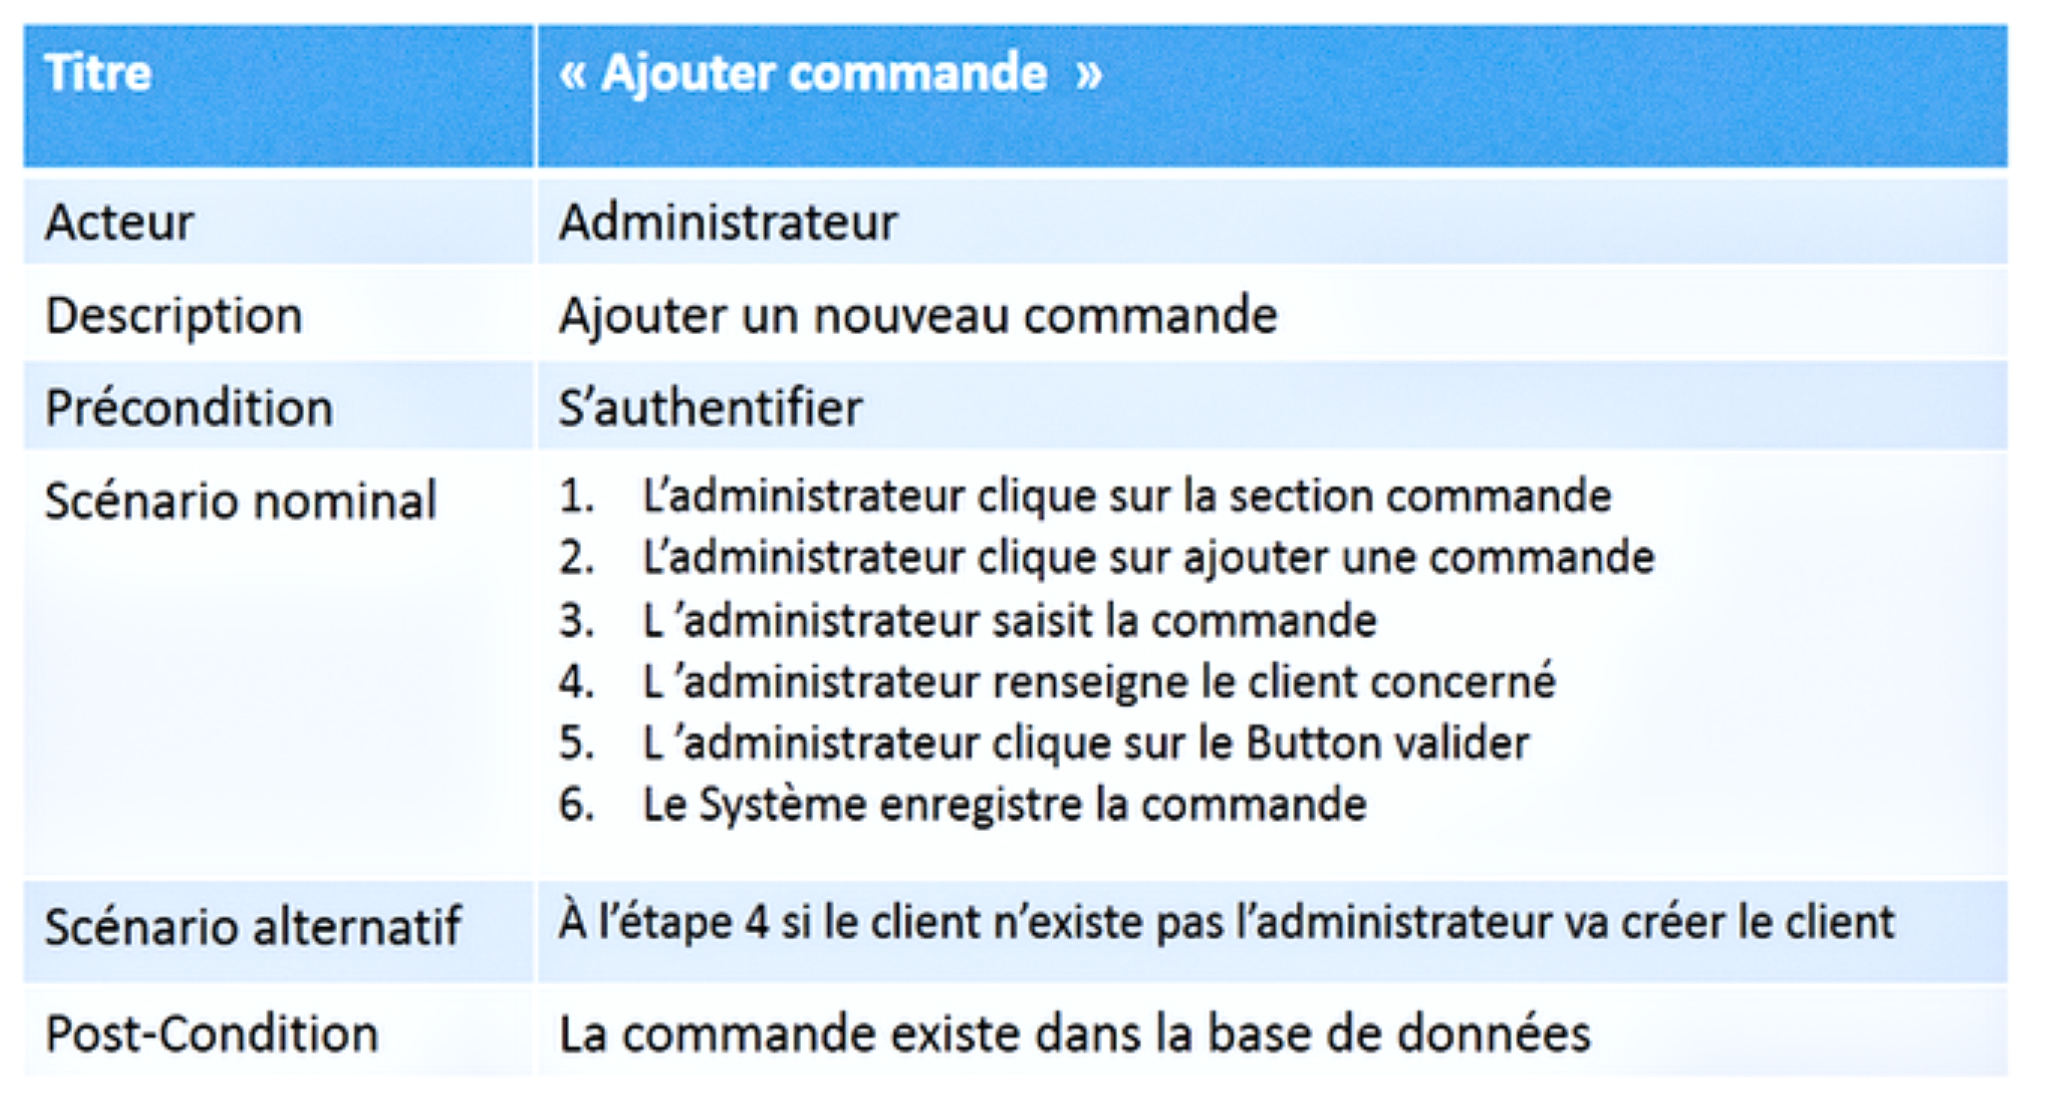
\includegraphics{img/fiche/8}
	\caption{Fiche textuelle du cas "Ajouter commande"}
	\label{Tux}
\end{table}

\begin{table}[H]
	\centering
	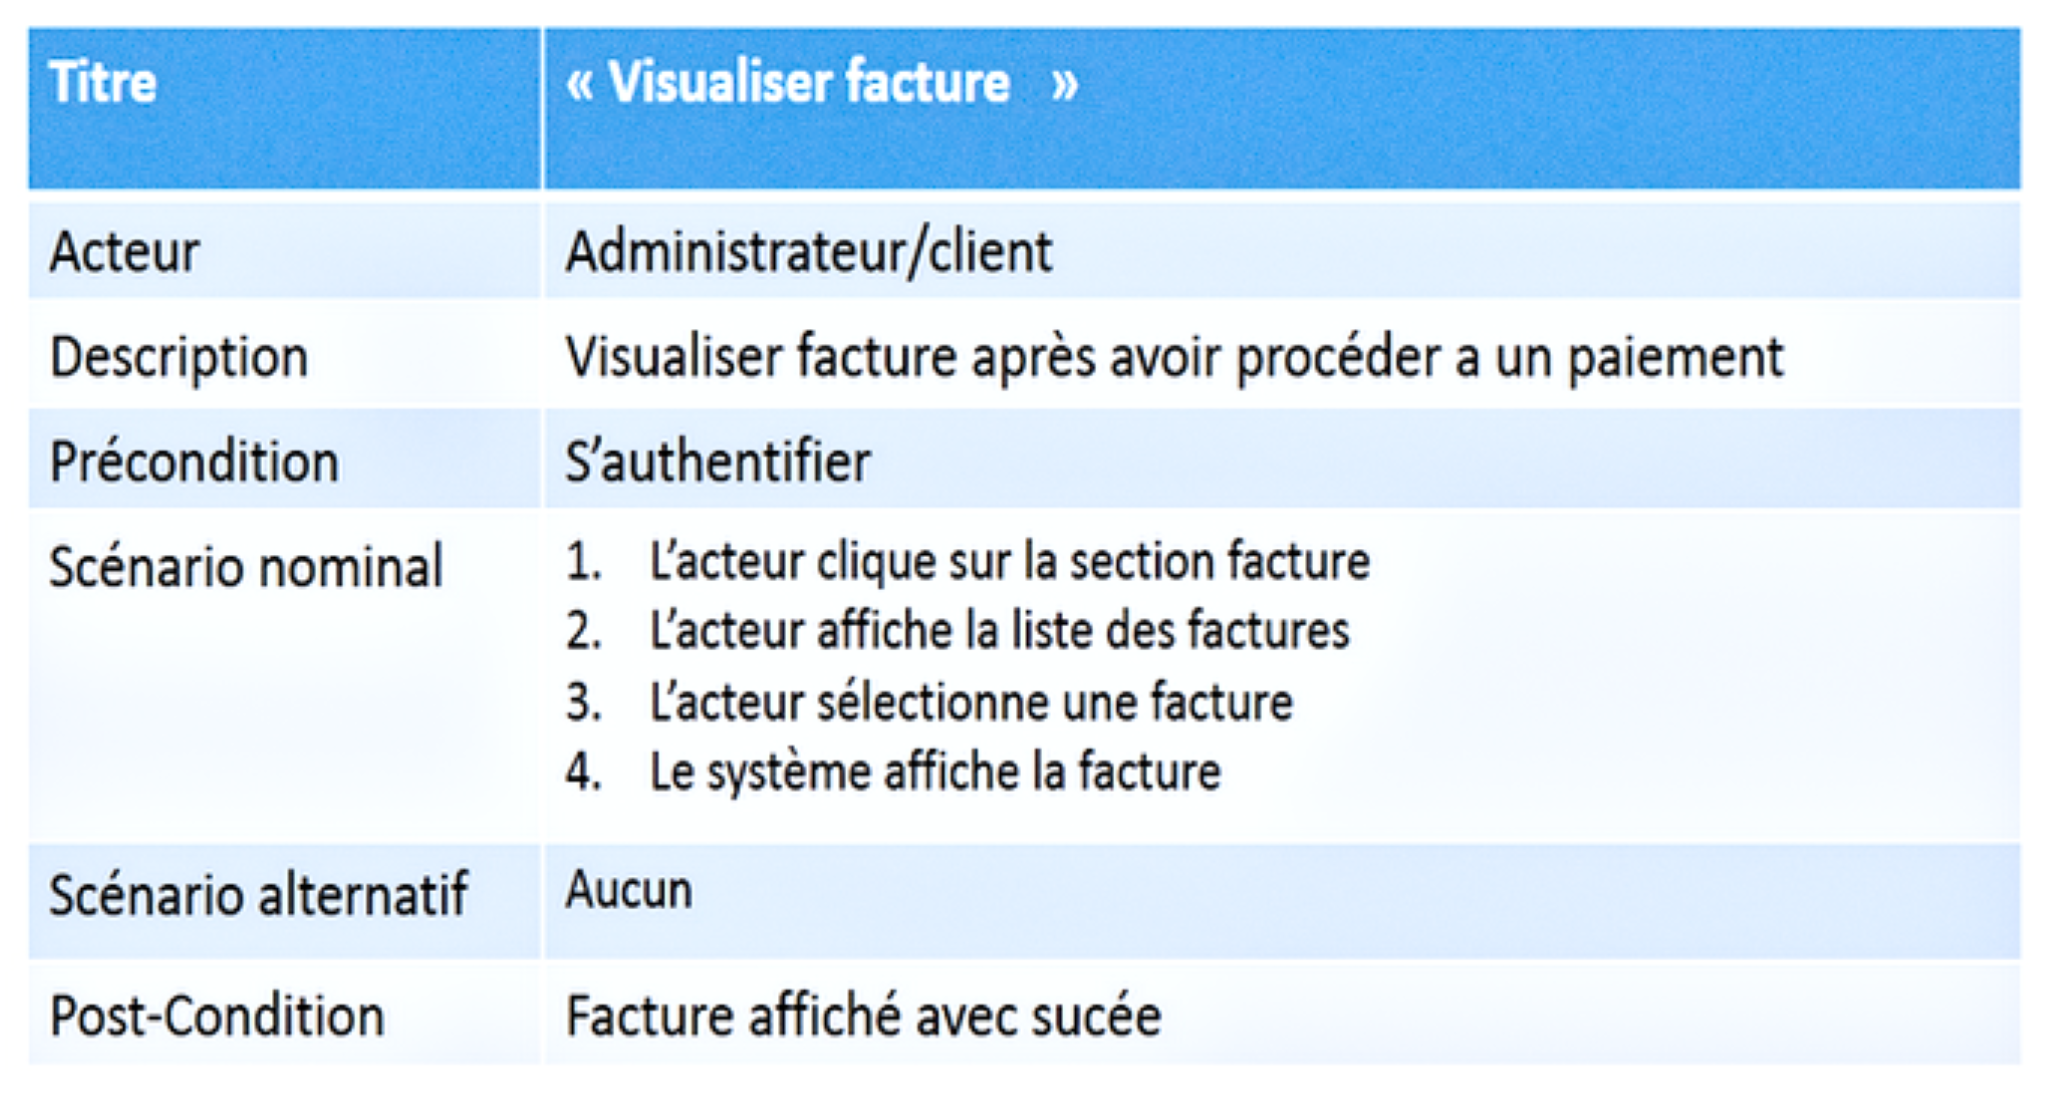
\includegraphics{img/fiche/9}
	\caption{Fiche textuelle du cas "Visualiser facture"}
	\label{Tux}
\end{table}
\begin{table}[H]
	\centering
	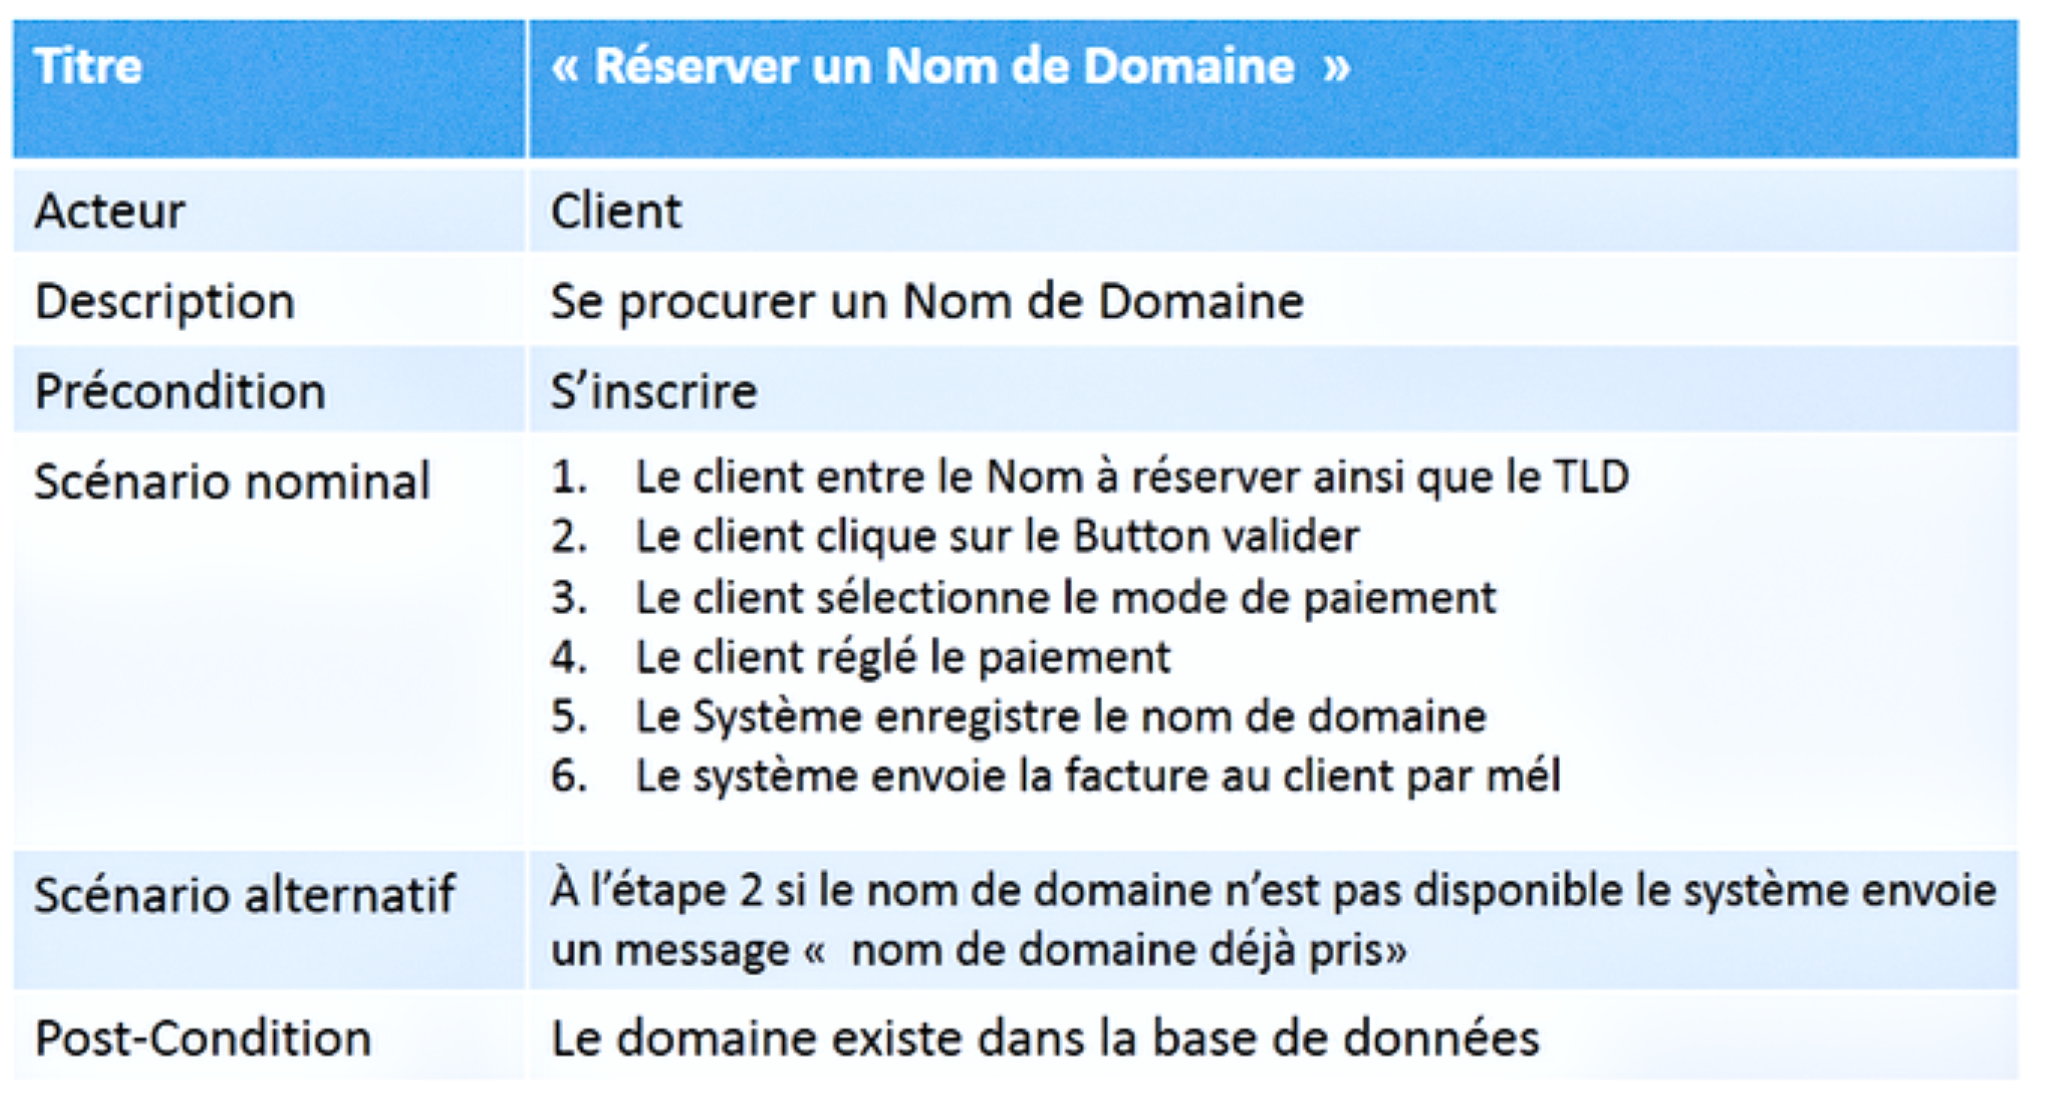
\includegraphics{img/fiche/10}
	\caption{Fiche textuelle du cas "Réserver un nom de domaine" }
	\label{Tux}
\end{table}
\begin{table}[H]
	\centering
	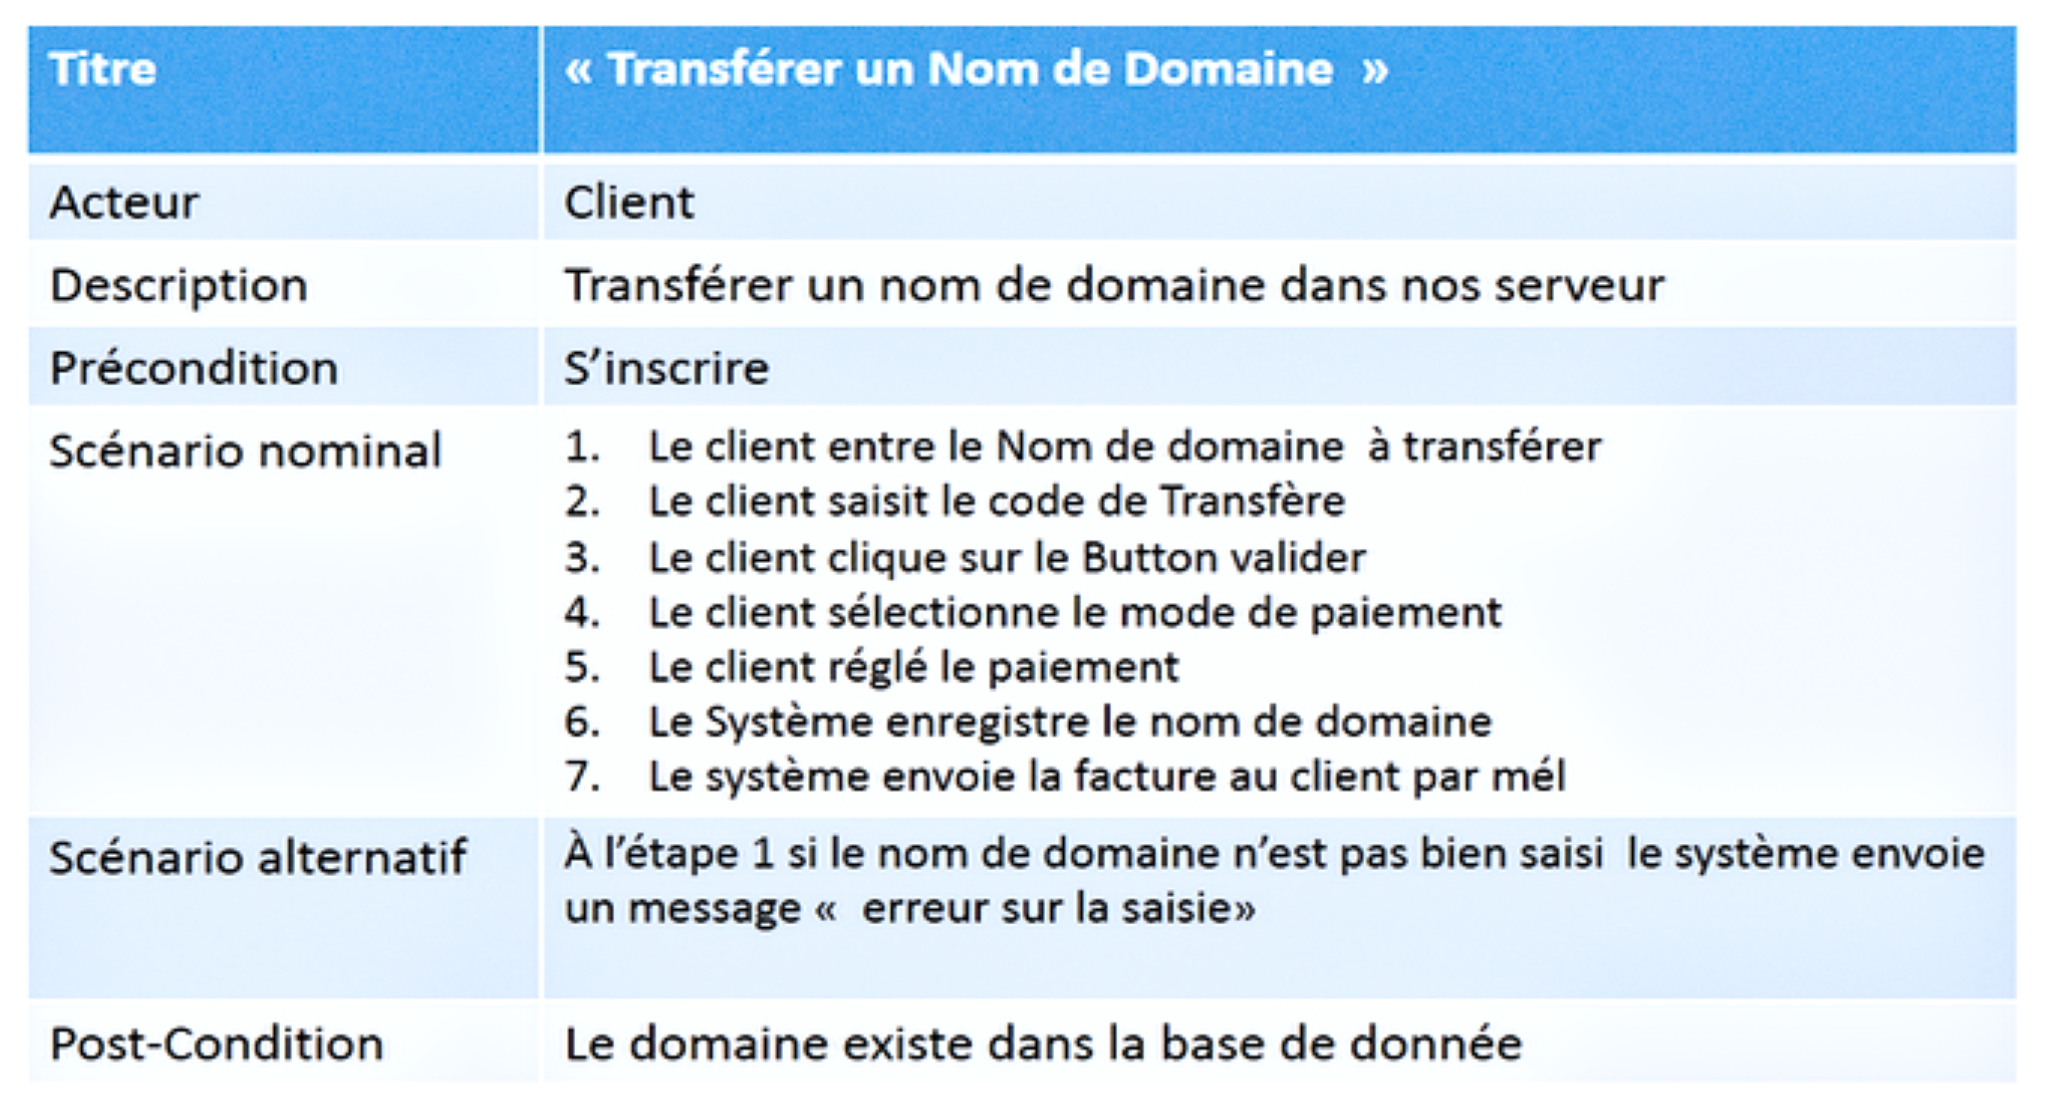
\includegraphics{img/fiche/11}
	\caption{Fiche textuelle du cas "Transférer un nom de domaine"}
	\label{Tux}
\end{table}
\begin{table}[H]
	\centering
	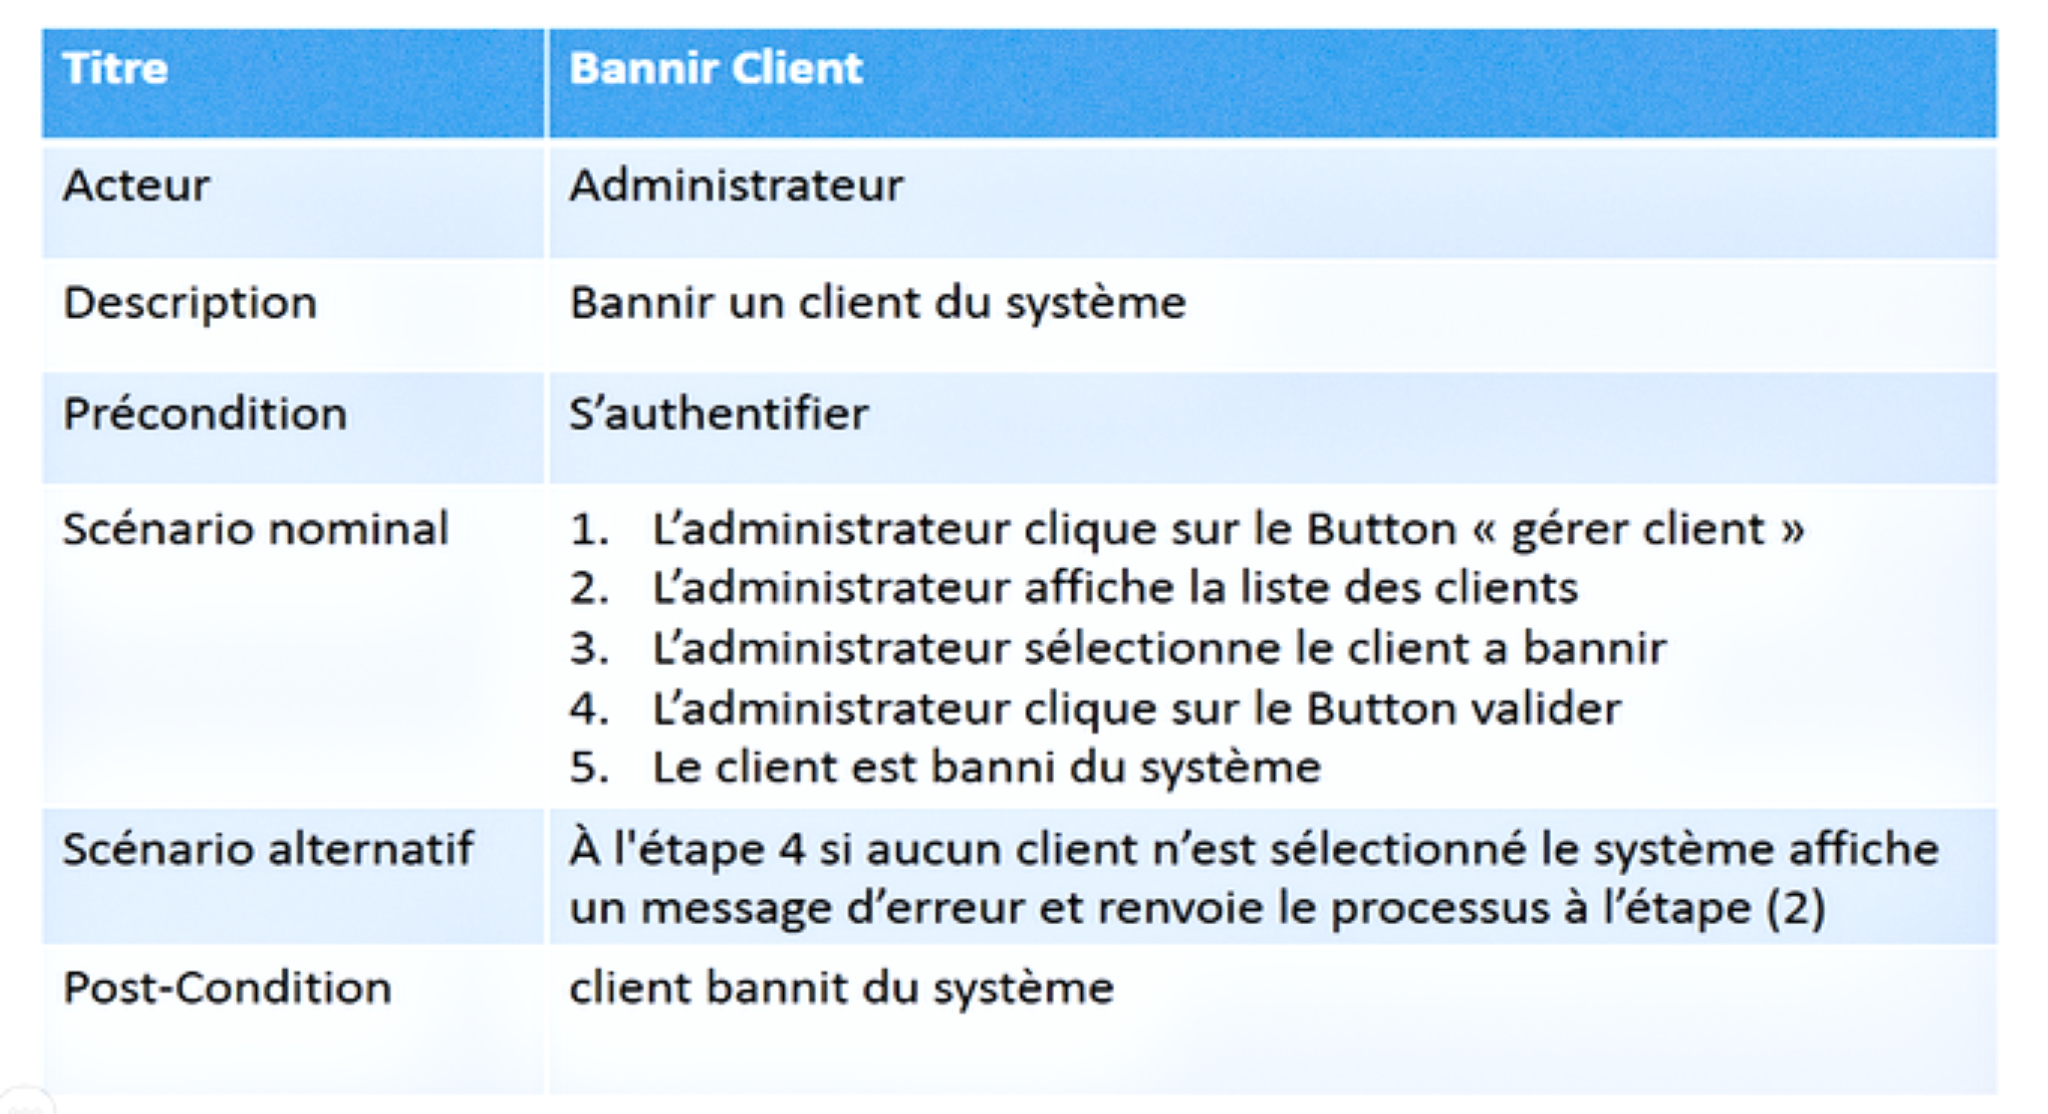
\includegraphics{img/fiche/12}
	\caption{Fiche textuelle du cas "Bannir client"}
	\label{Tux}
\end{table}
\begin{table}[H]
	\centering
	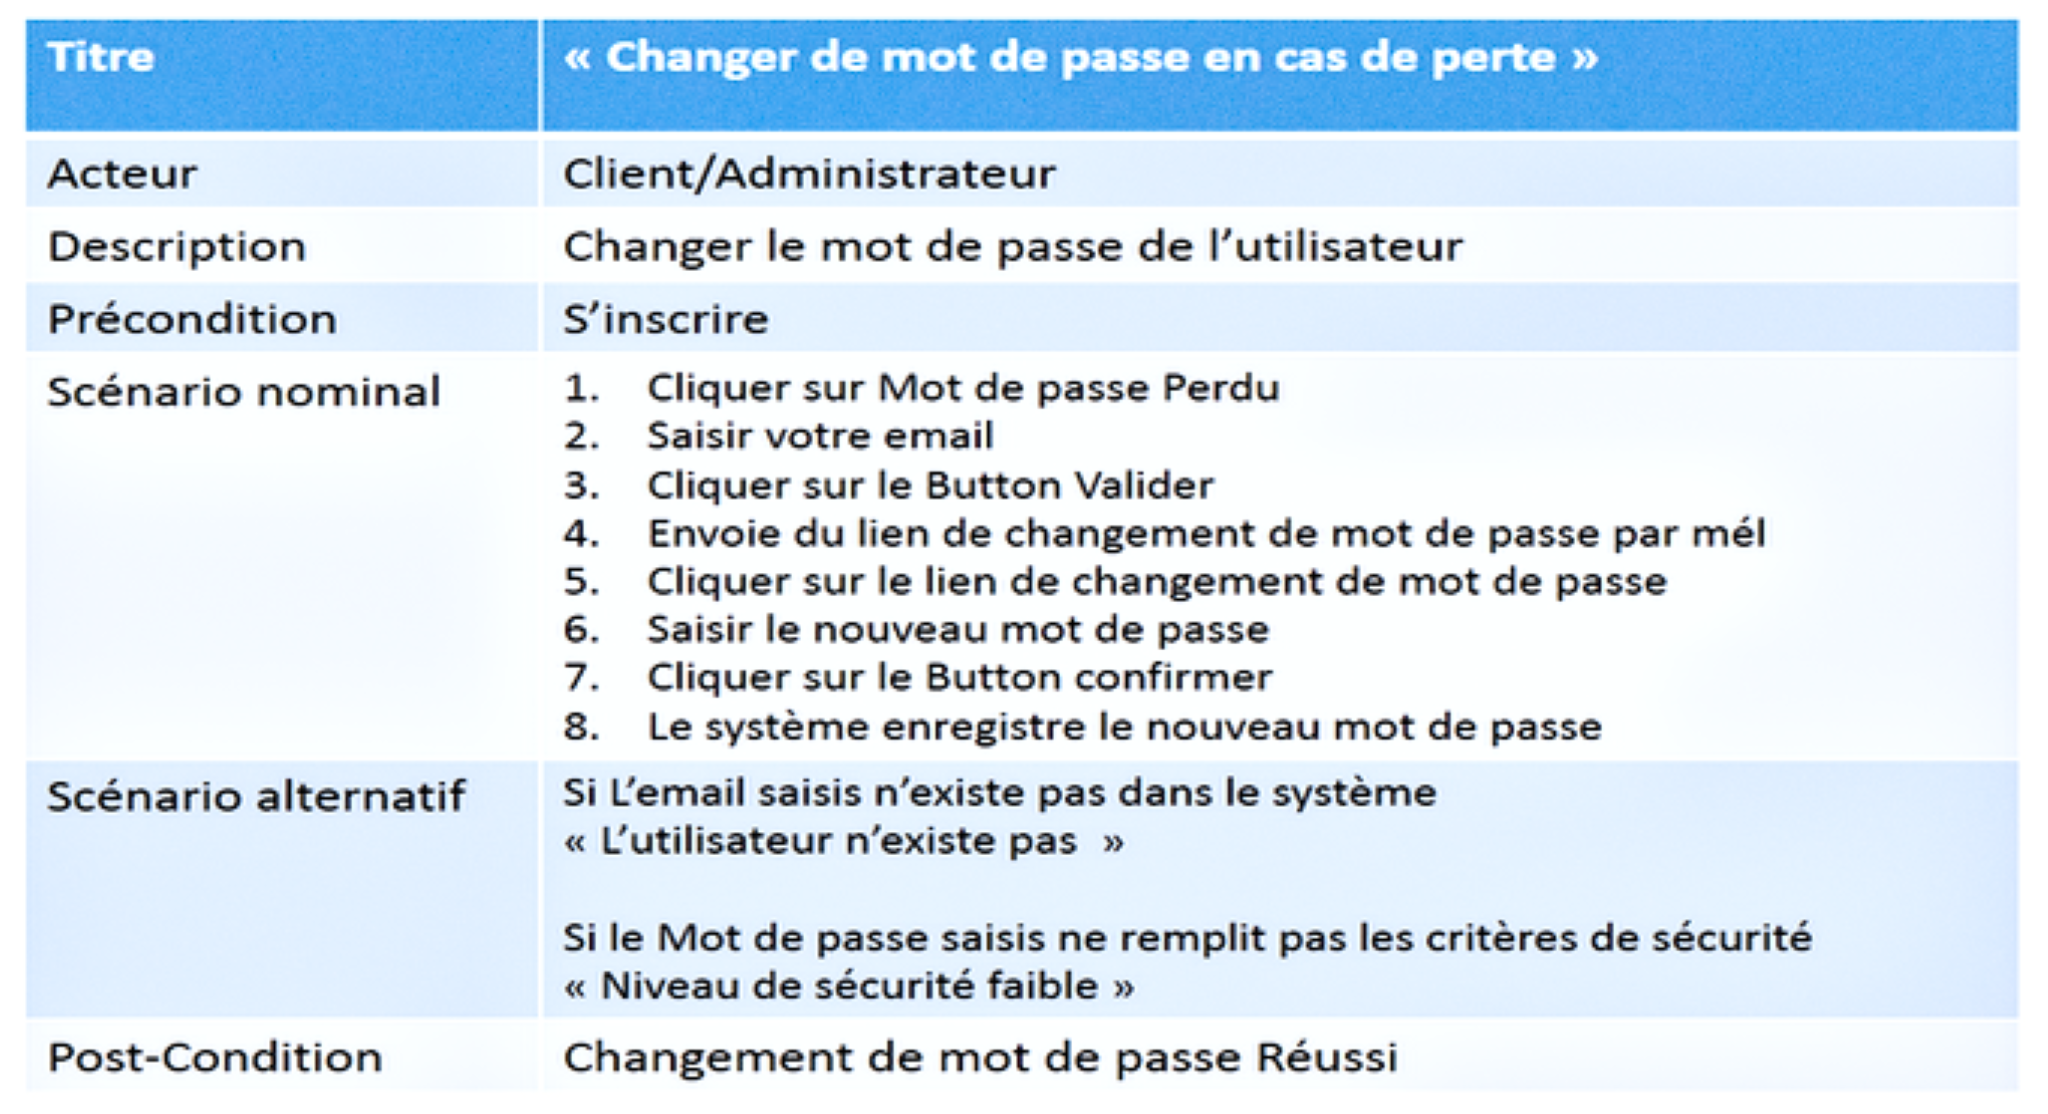
\includegraphics{img/fiche/13}
	\caption{Fiche textuelle du cas "changer de mot de passe en cas de perte "}
	\label{Tux}
\end{table}
\begin{table}[H]
	\centering
	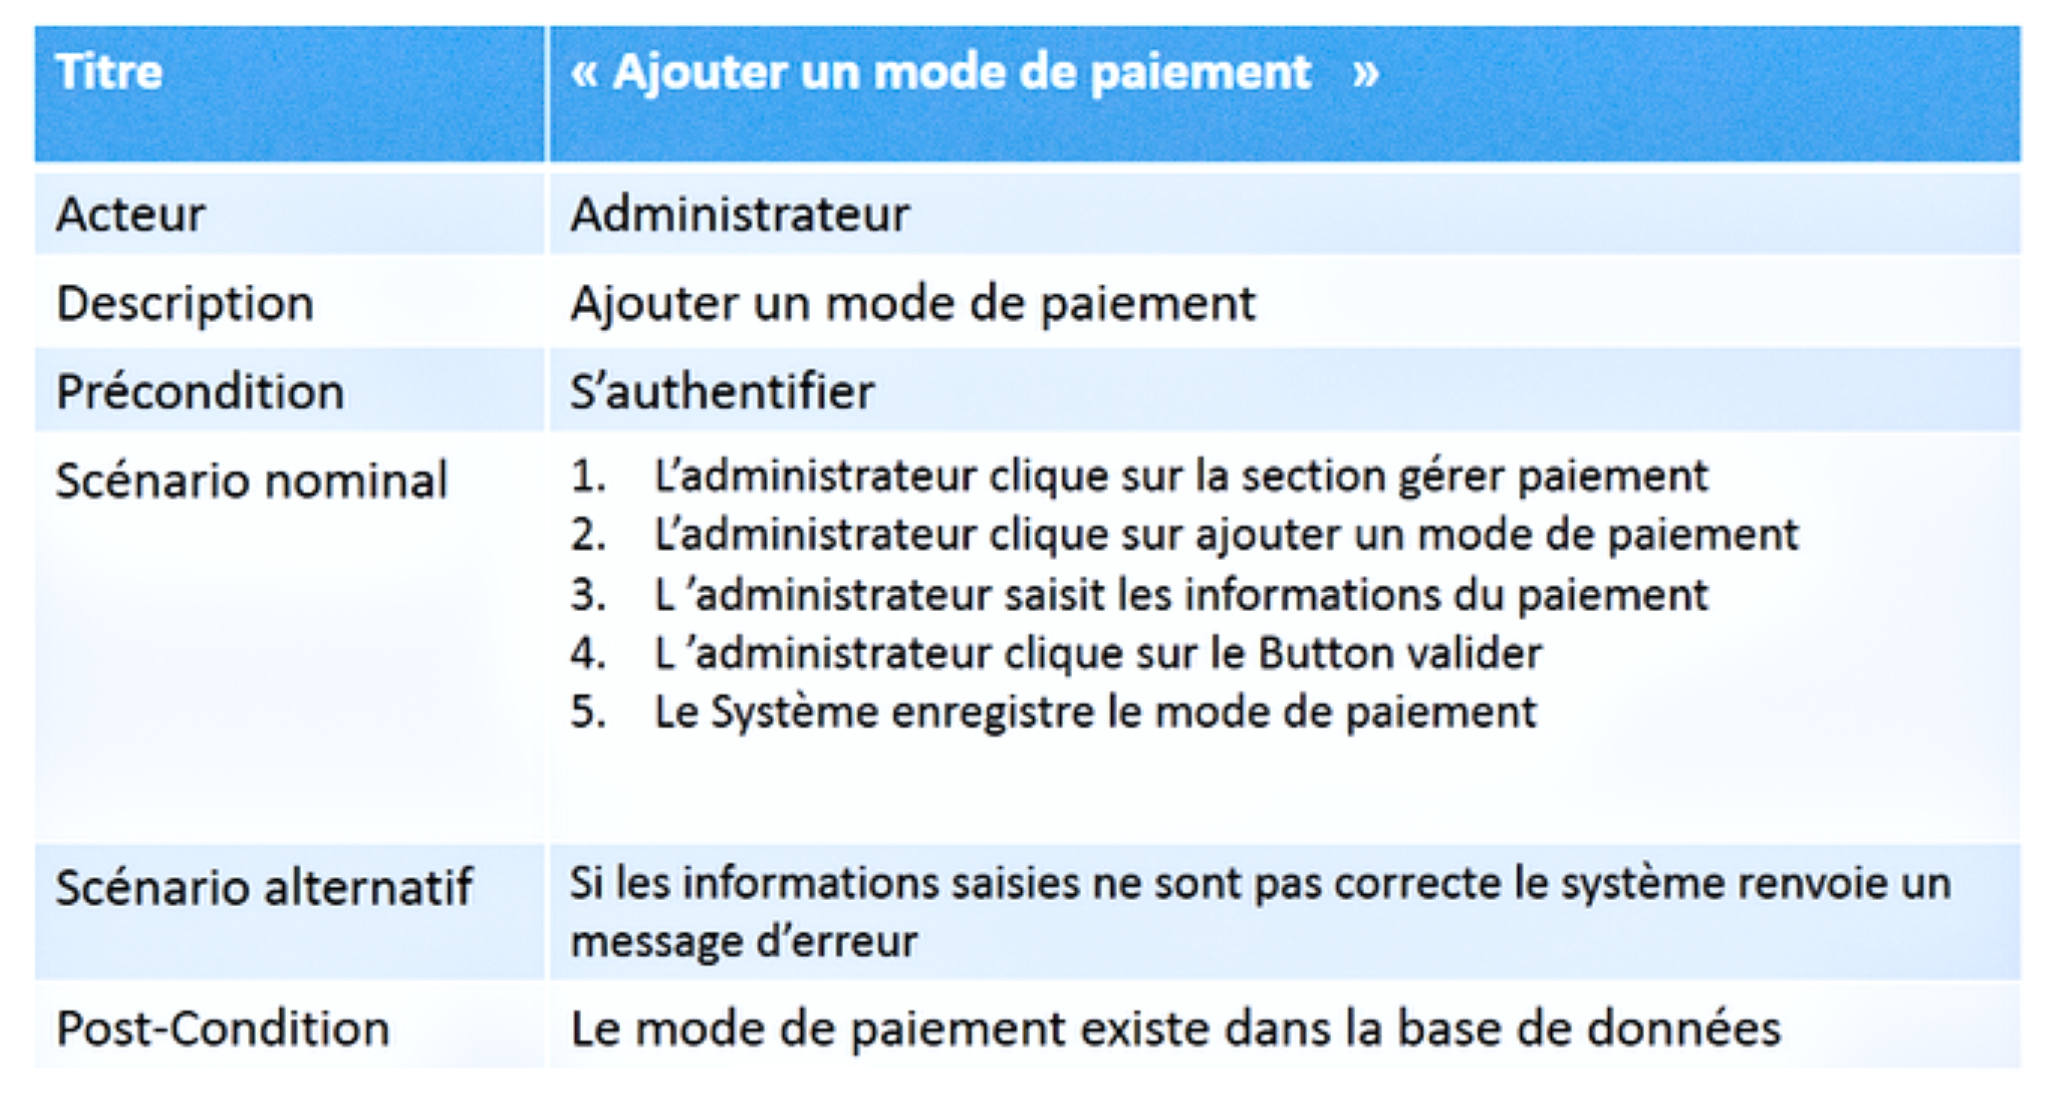
\includegraphics{img/fiche/14}
	\caption{Fiche textuelle du cas "Ajouter un mode de paiement"}
	\label{Tux}
\end{table}
\begin{table}[H]
	\centering
	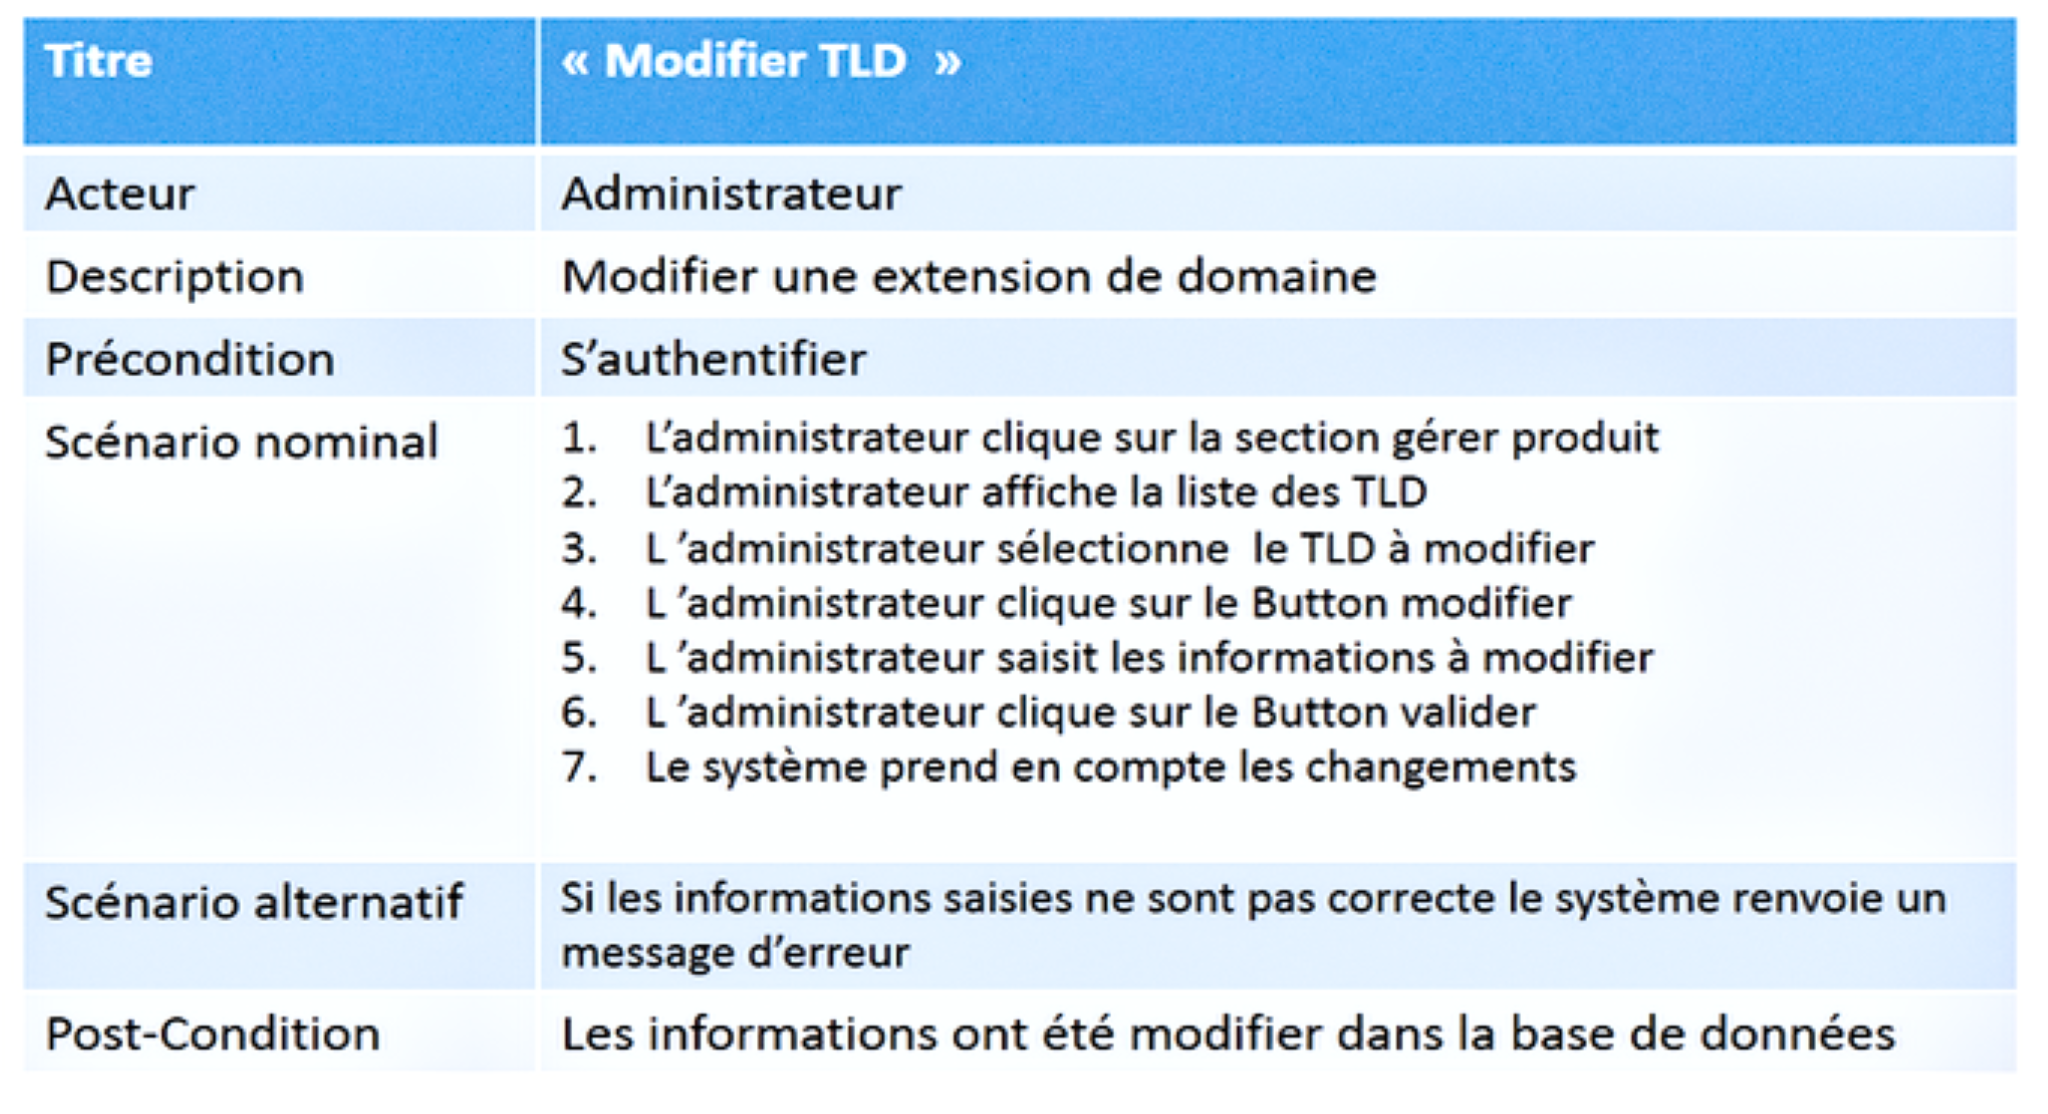
\includegraphics{img/fiche/15}
	\caption{Fiche textuelle du cas "Modifier TLD (top-level-domain)"}
	\label{Tux}
\end{table}
\begin{table}[H]
	\centering
	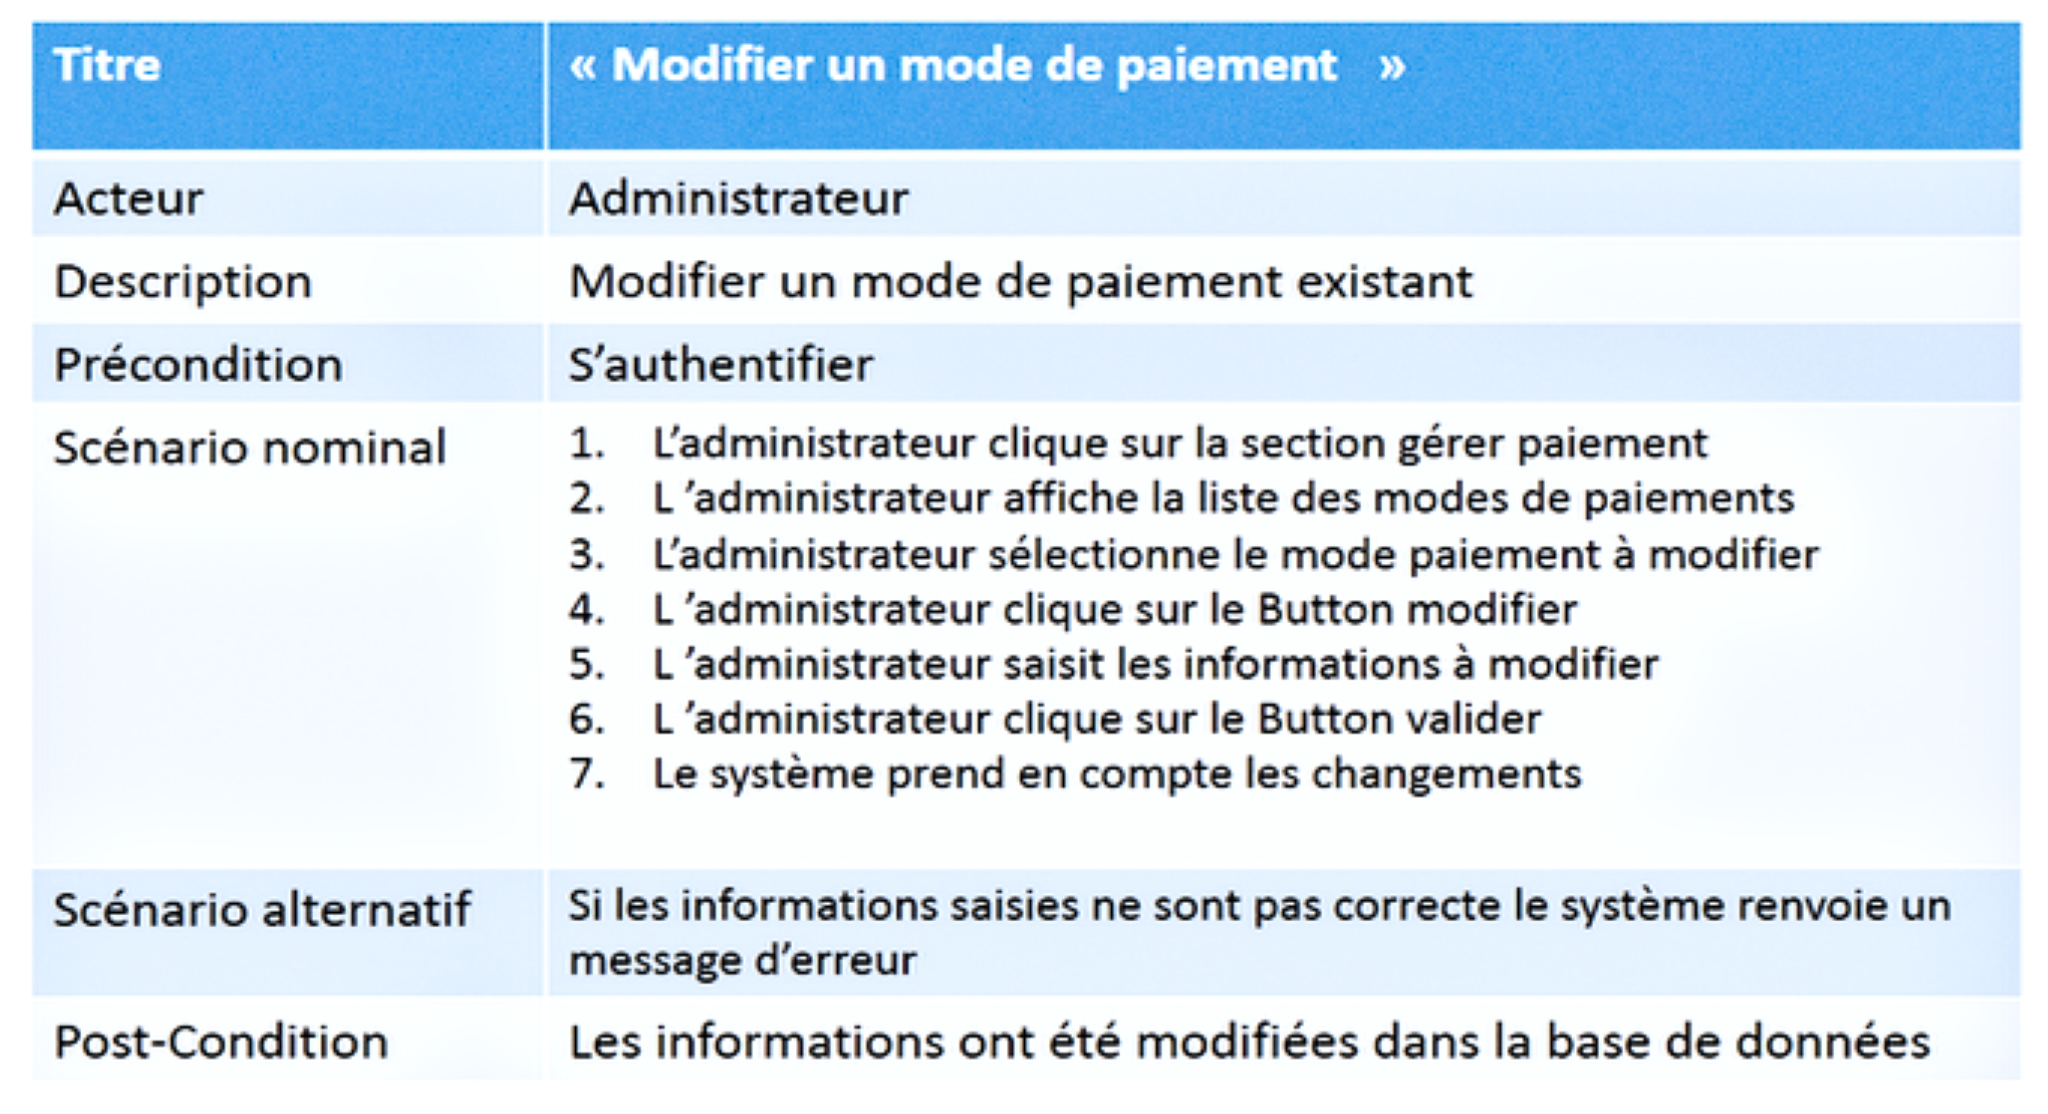
\includegraphics{img/fiche/16}
	\caption{Fiche textuelle du cas "Modifier un mode de paiement "}
	\label{Tux}
\end{table}
\begin{table}[H]
	\centering
	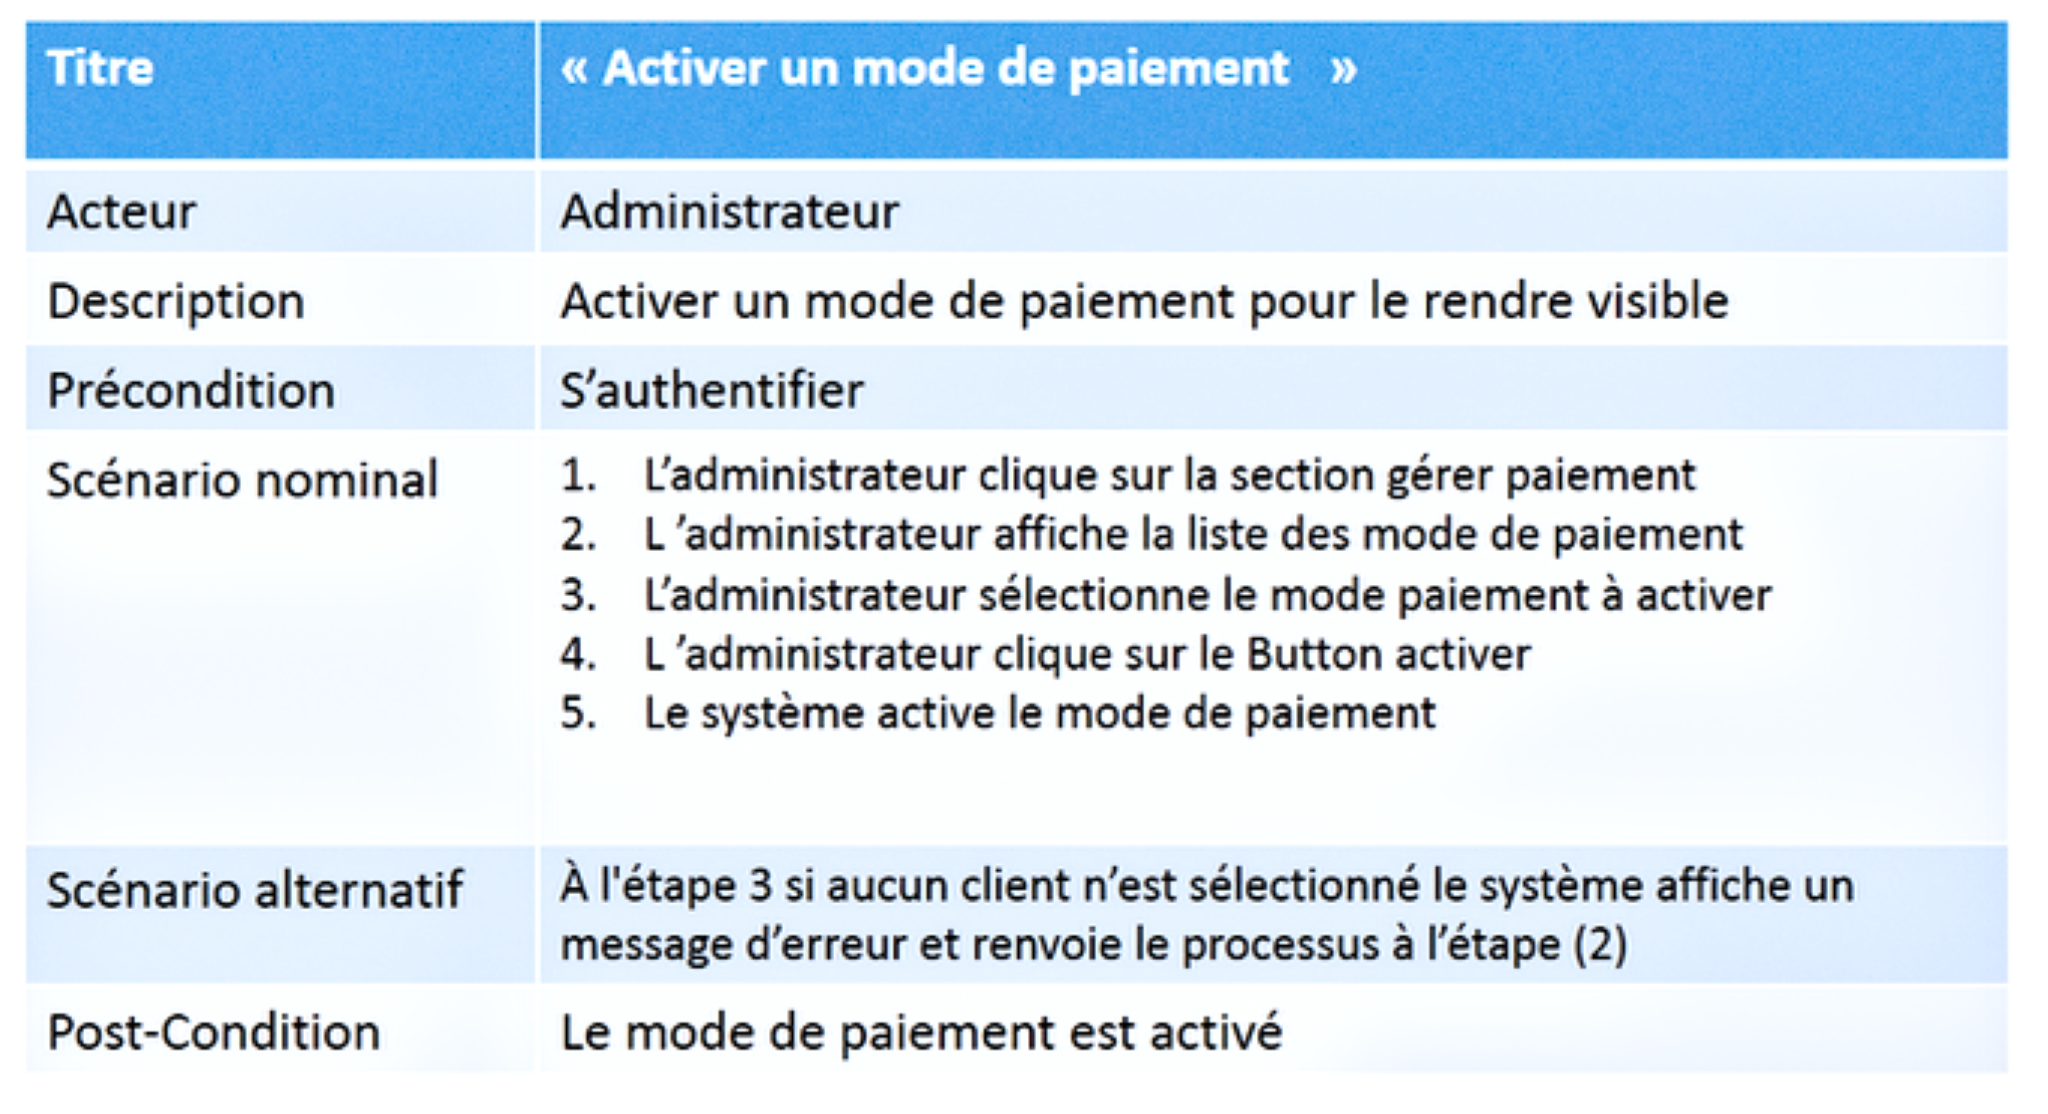
\includegraphics{img/fiche/17}
	\caption{Fiche textuelle du cas "Activer un mode de paiement"}
	\label{Tux}
\end{table}
\begin{table}[H]
	\centering
	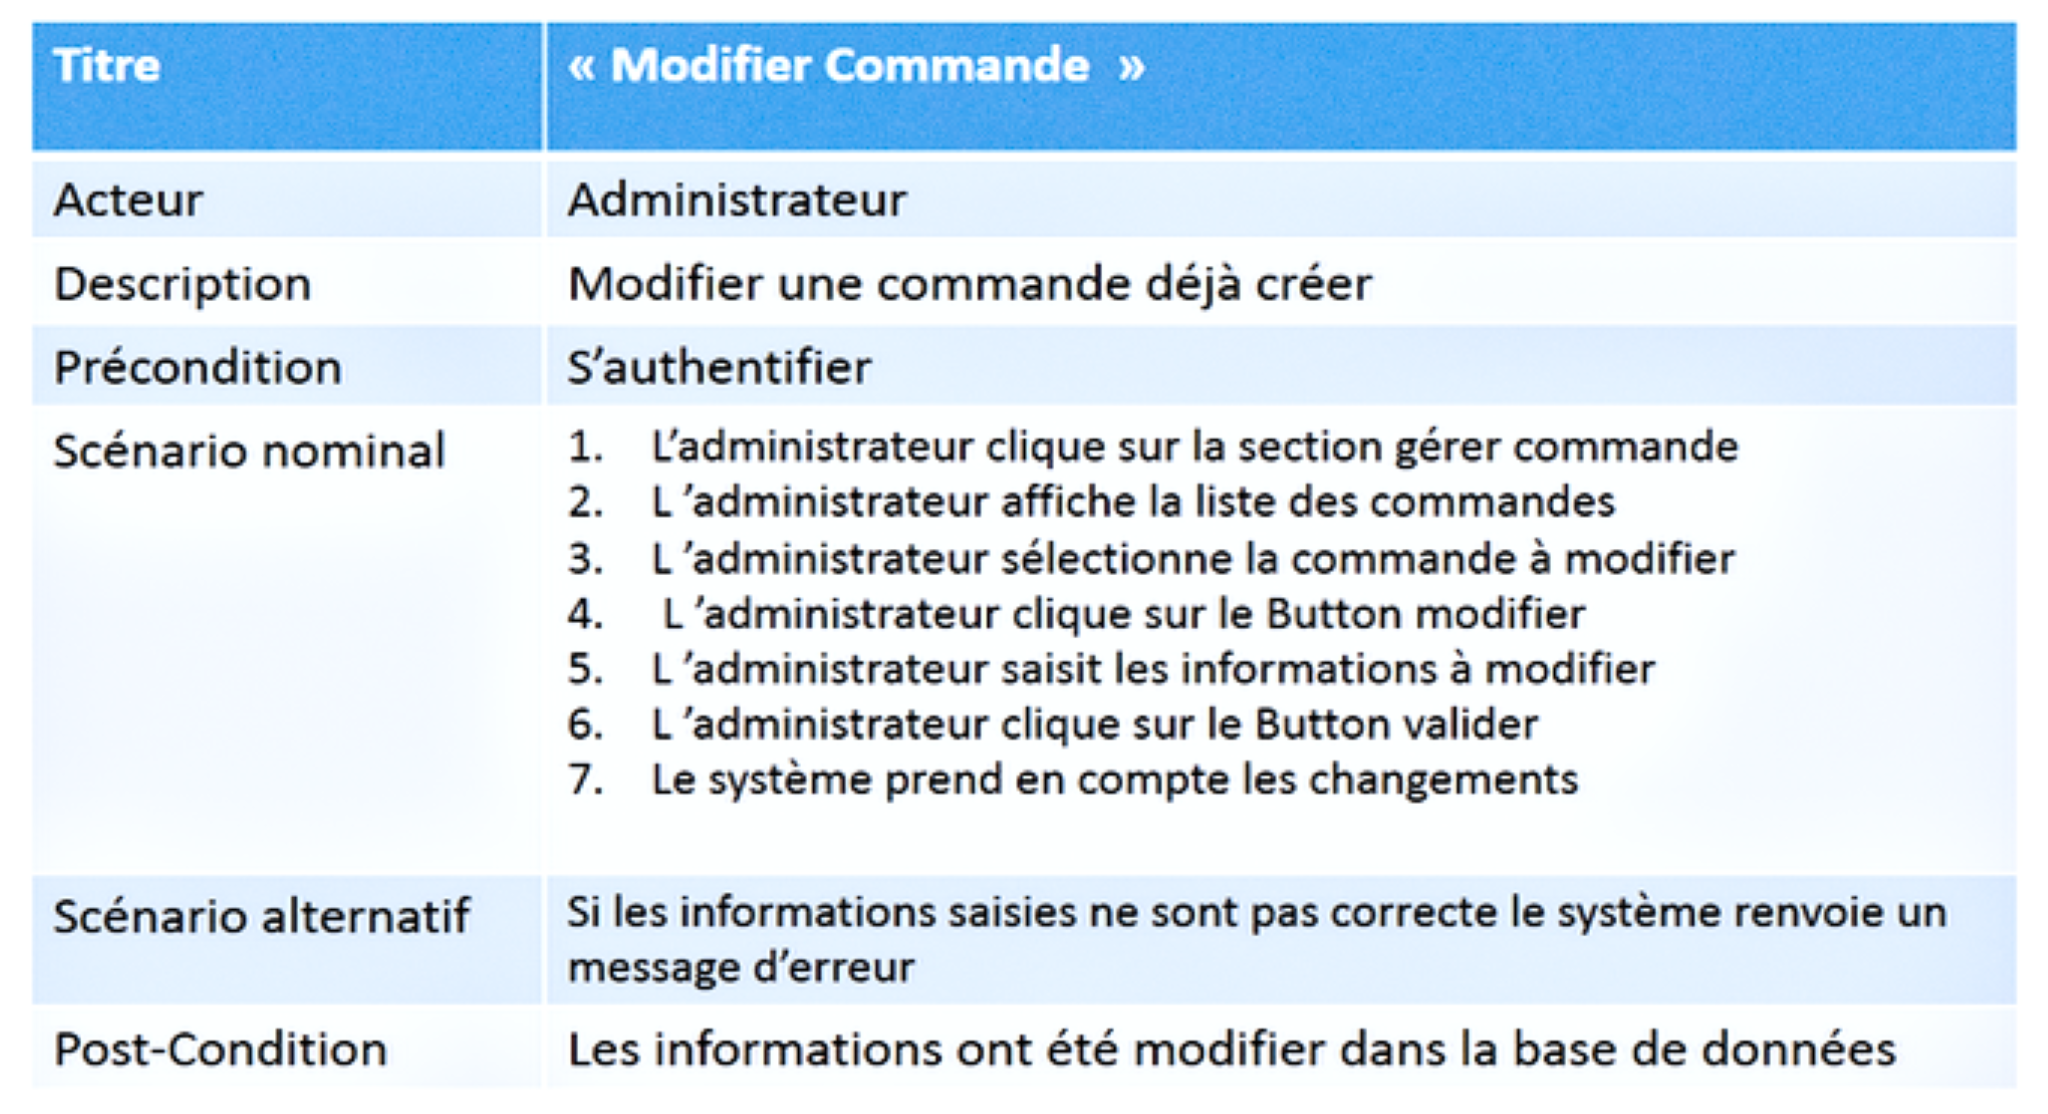
\includegraphics{img/fiche/18}
	\caption{Fiche textuelle du cas "Modifier commande"}
	\label{Tux}
\end{table}
\begin{table}[H]
	\centering
	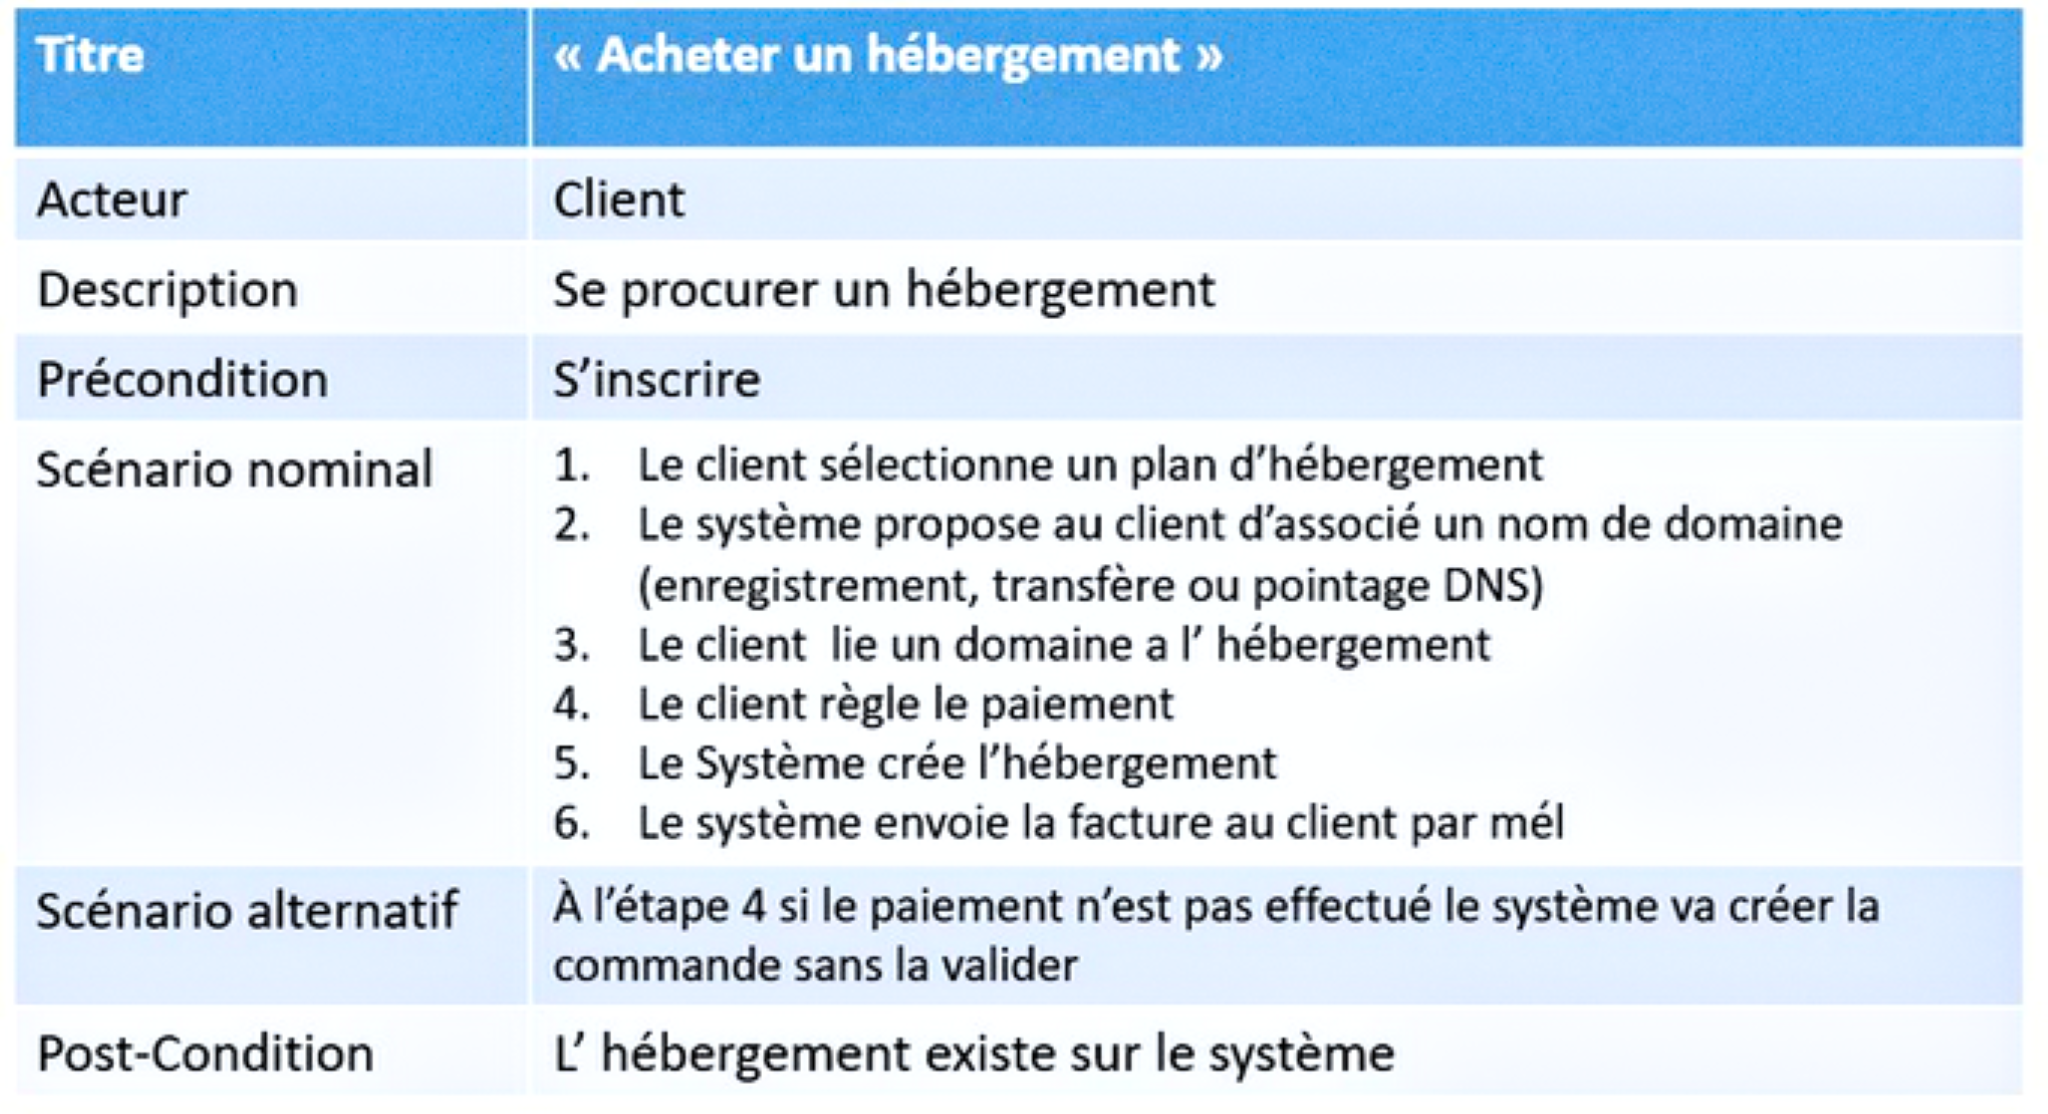
\includegraphics{img/fiche/19}
	\caption{Fiche textuelle du cas "Prendre un Hebergement"}
	\label{Tux}
\end{table}
\begin{table}[H]
	\centering
	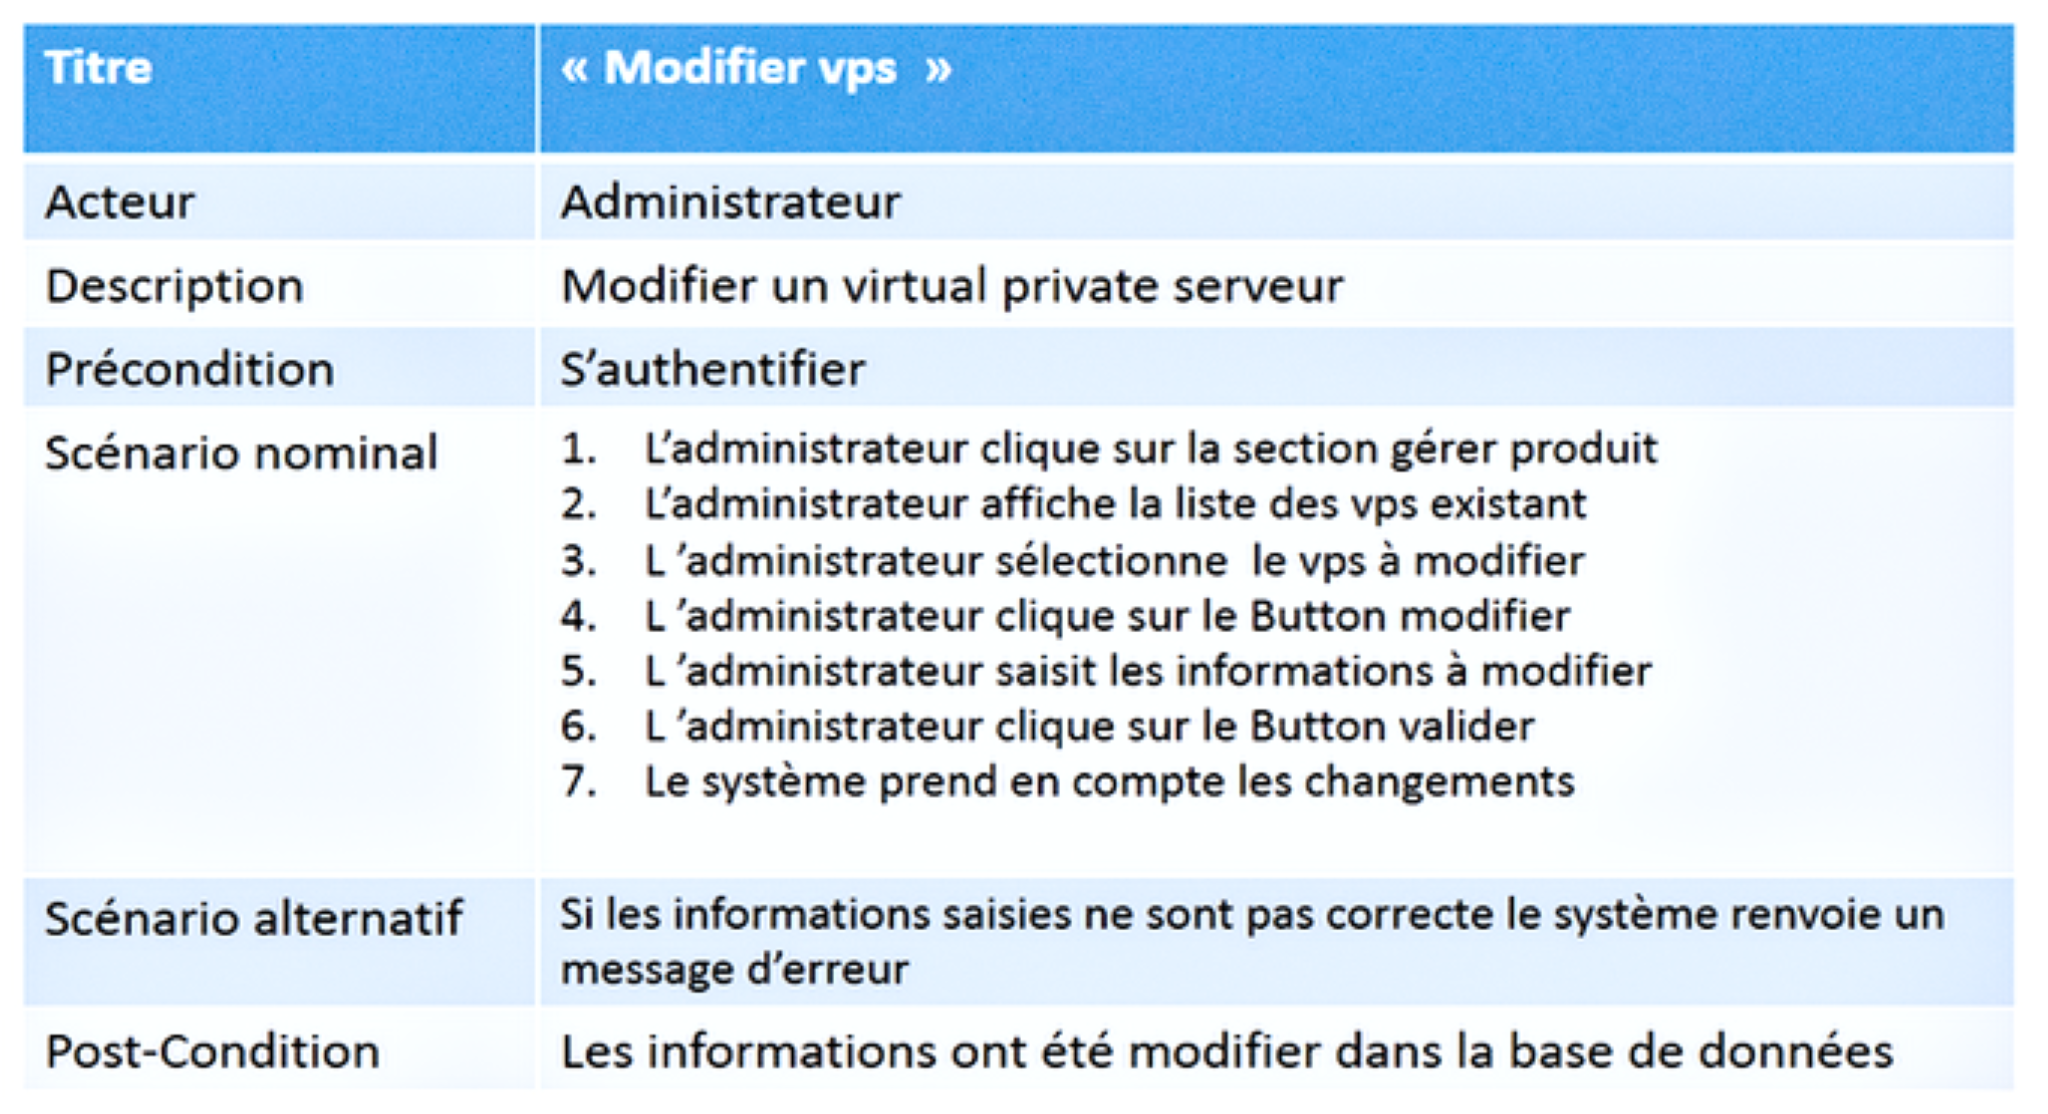
\includegraphics{img/fiche/20}
	\caption{Fiche textuelle du cas "modifier vps"}
	\label{Tux}
\end{table}
\begin{table}[H]
	\centering
	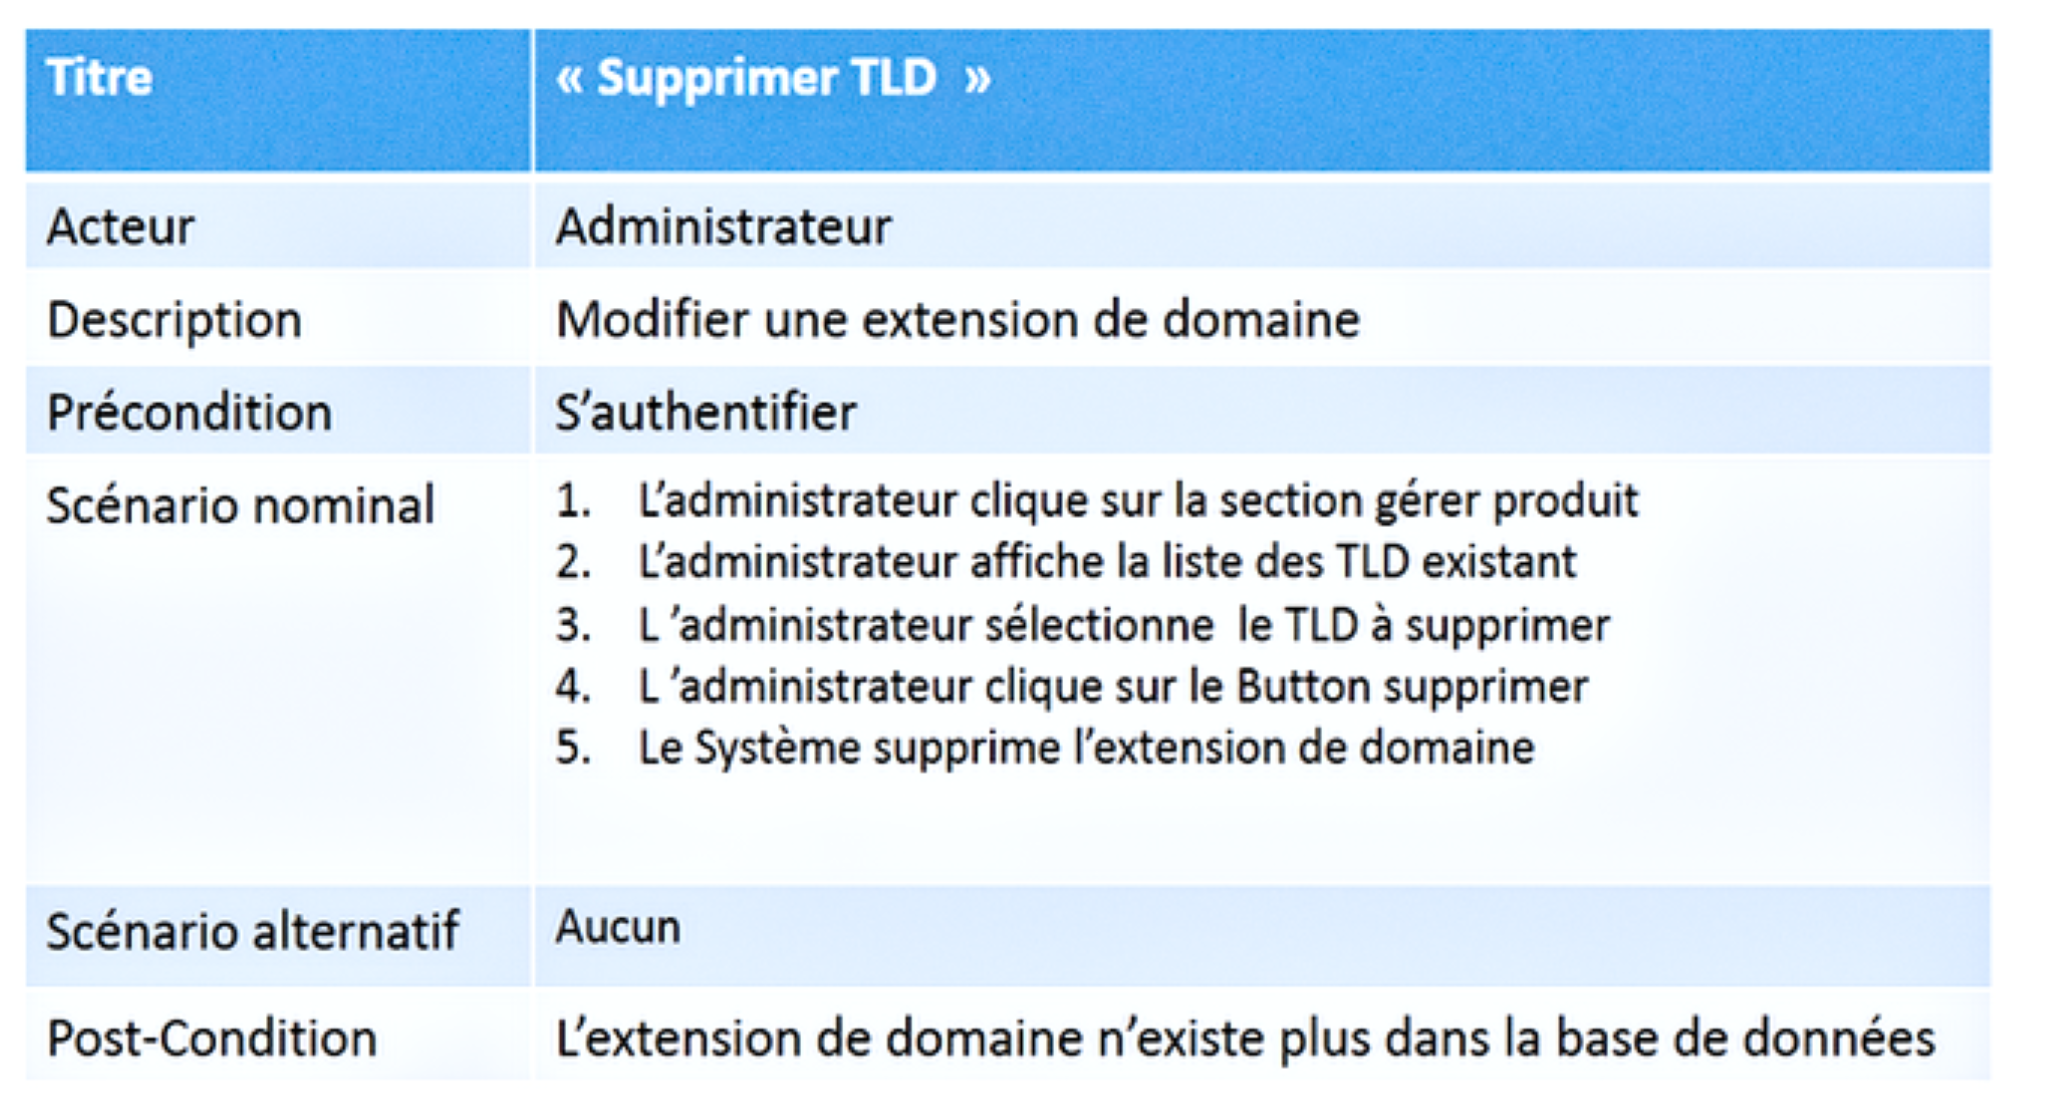
\includegraphics{img/fiche/21}
	\caption{Fiche textuelle du cas "supprimer tld"}
	\label{Tux}
\end{table}
\begin{table}[H]
	\centering
	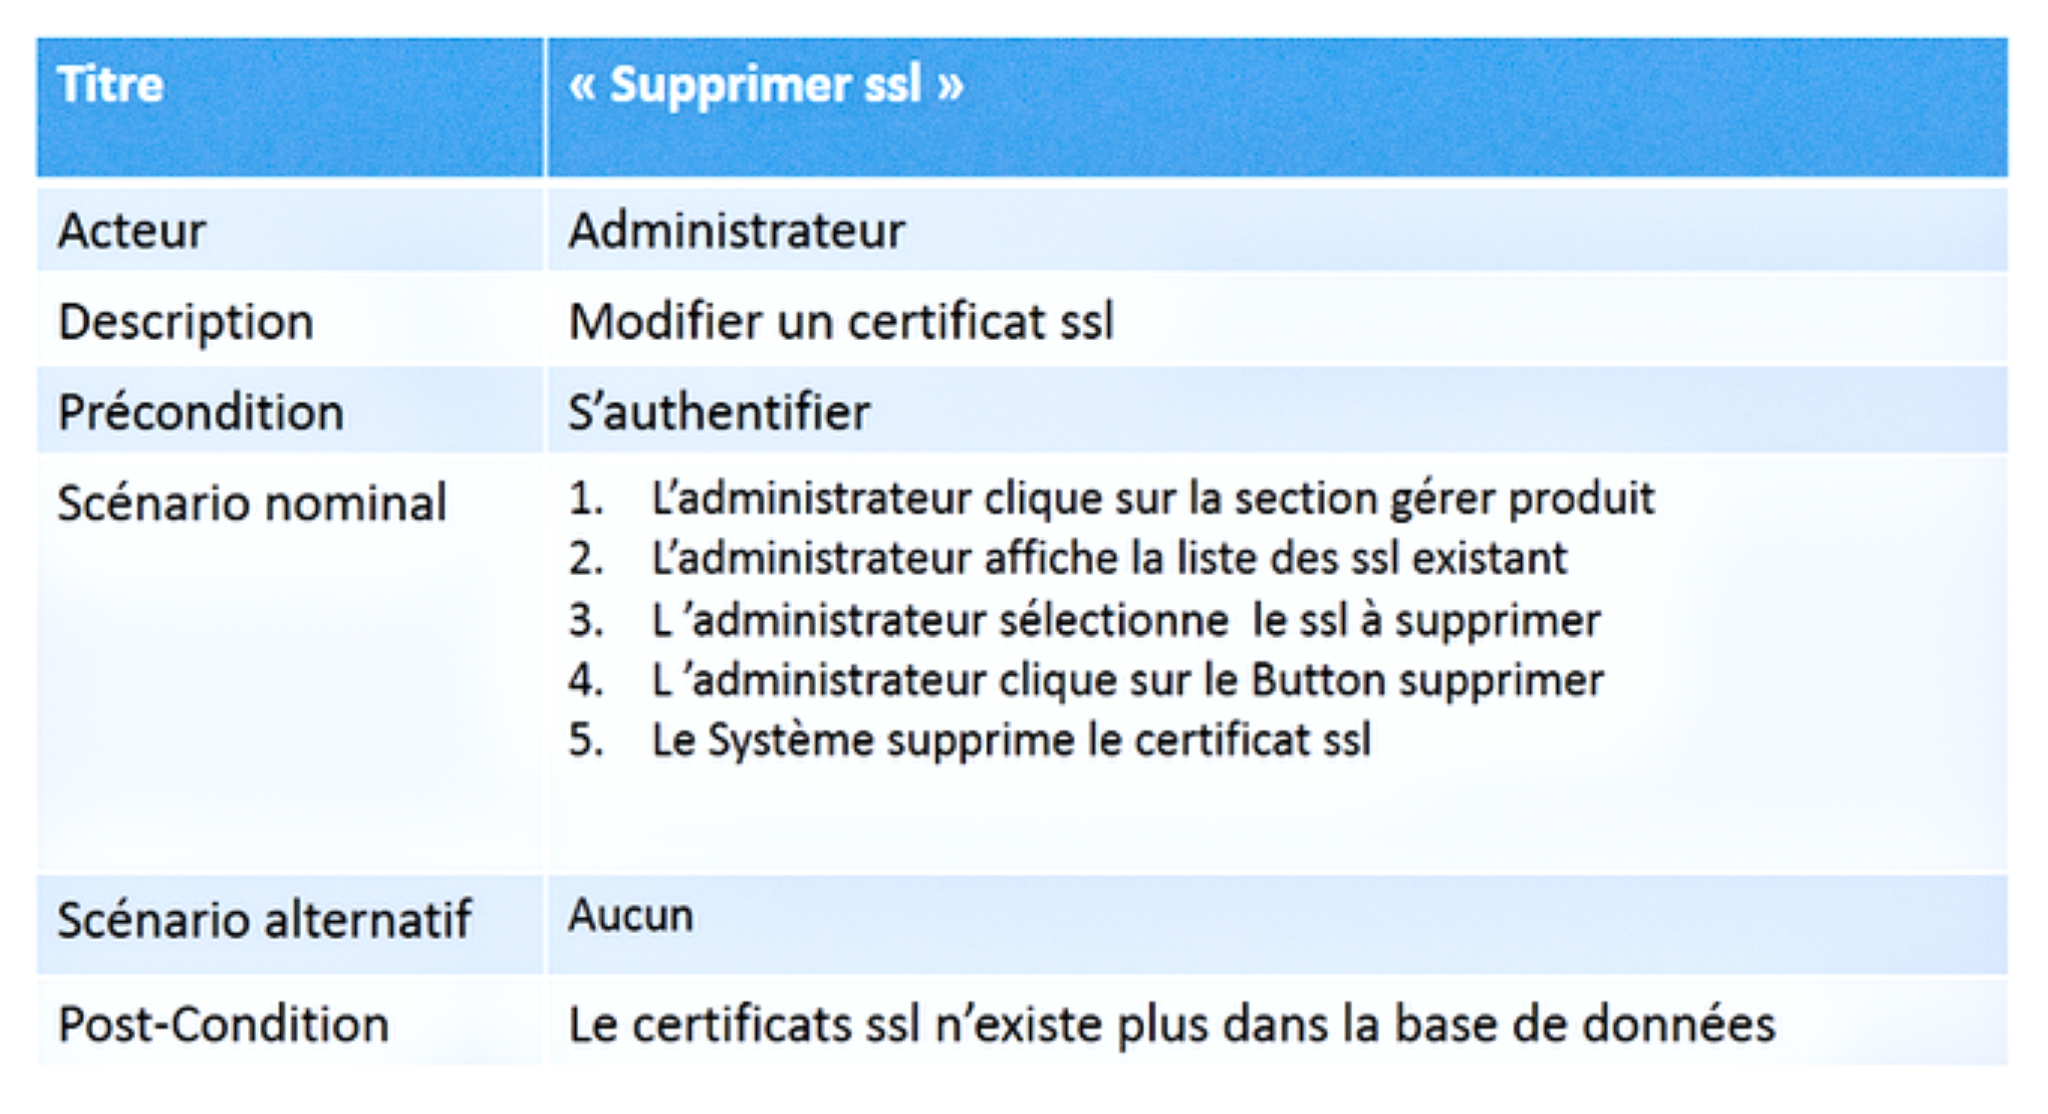
\includegraphics{img/fiche/22}
	\caption{Fiche textuelle du cas "supprimer ssl"}
	\label{Tux}
\end{table}
\begin{table}[H]
	\centering
	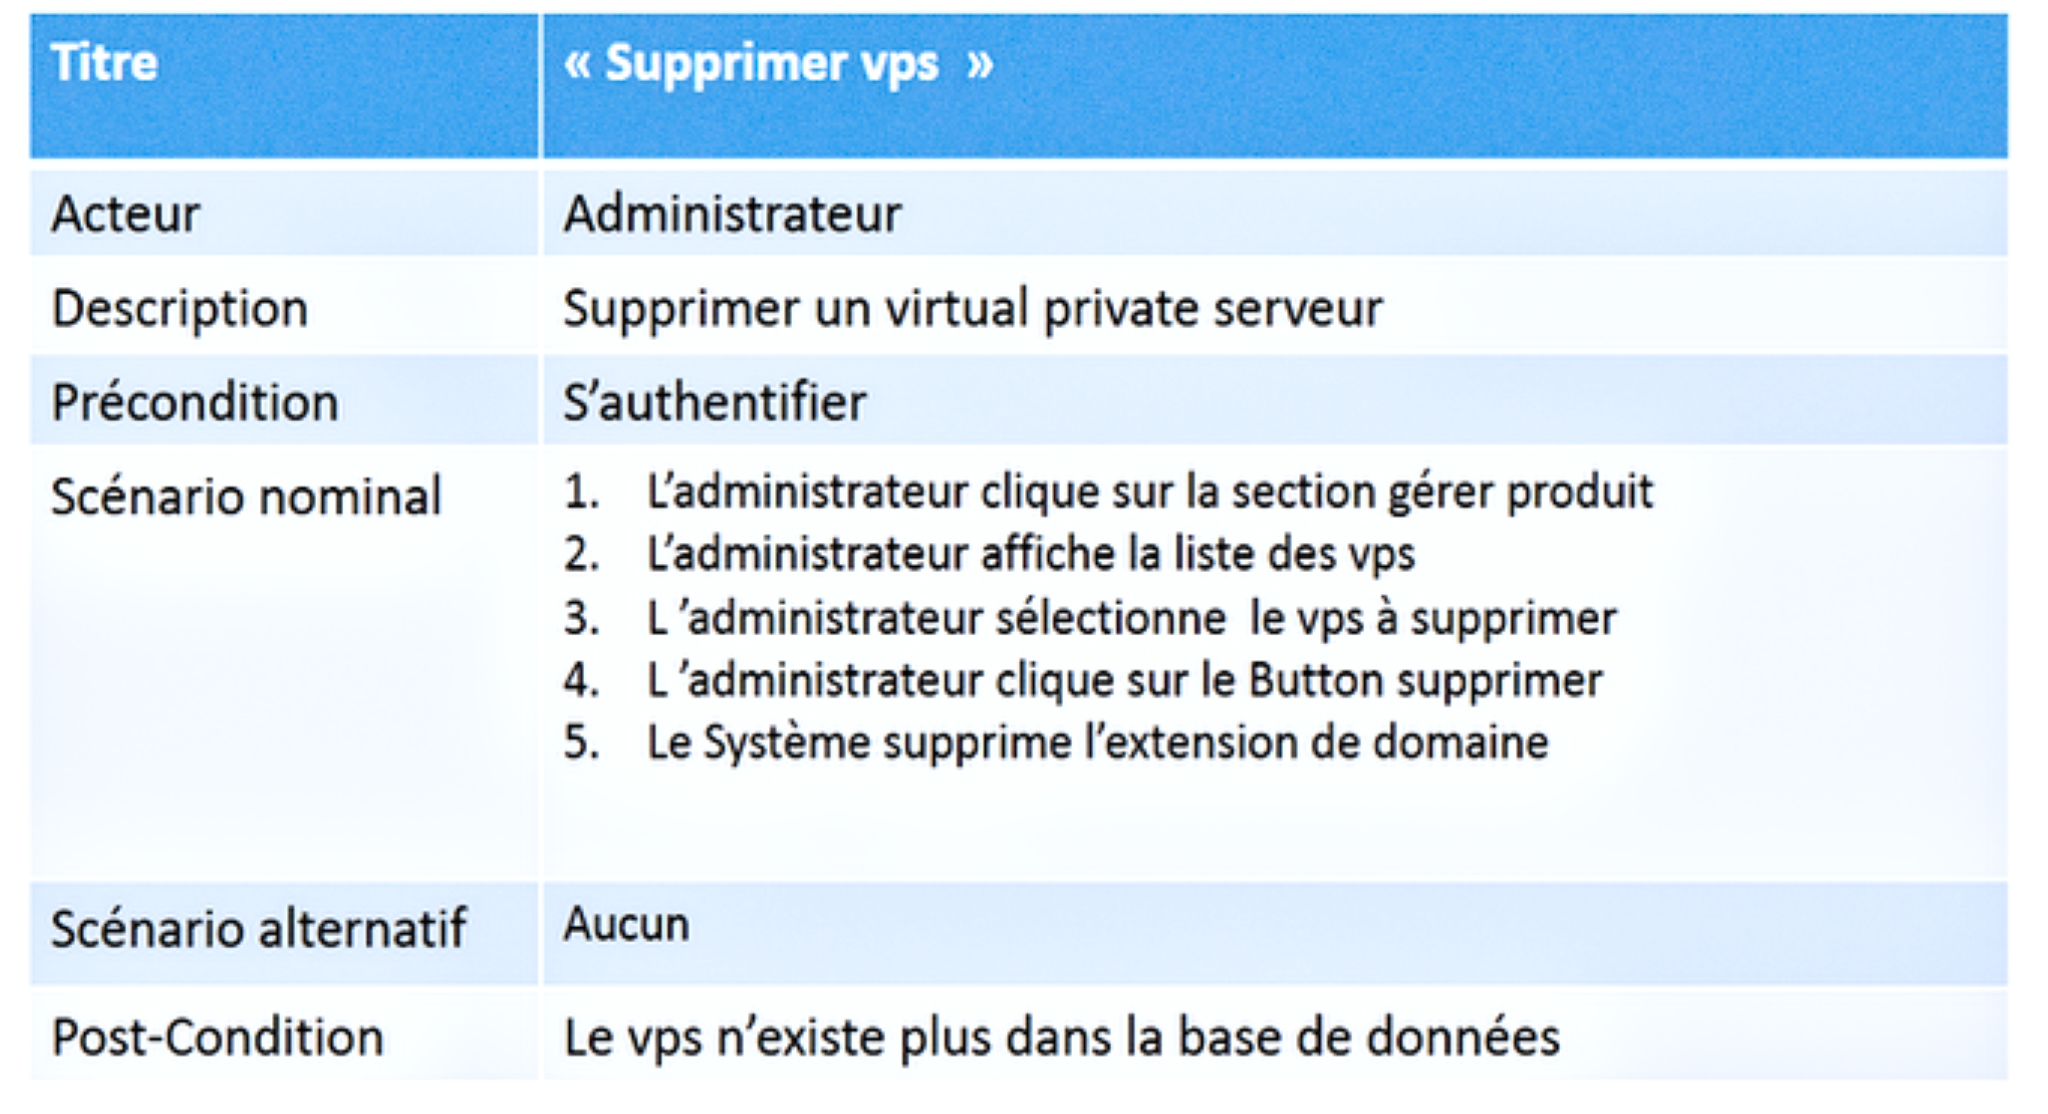
\includegraphics{img/fiche/23}
	\caption{Fiche textuelle du cas "supprimer vps" }
	\label{Tux}
\end{table}
\begin{table}[H]
	\centering
	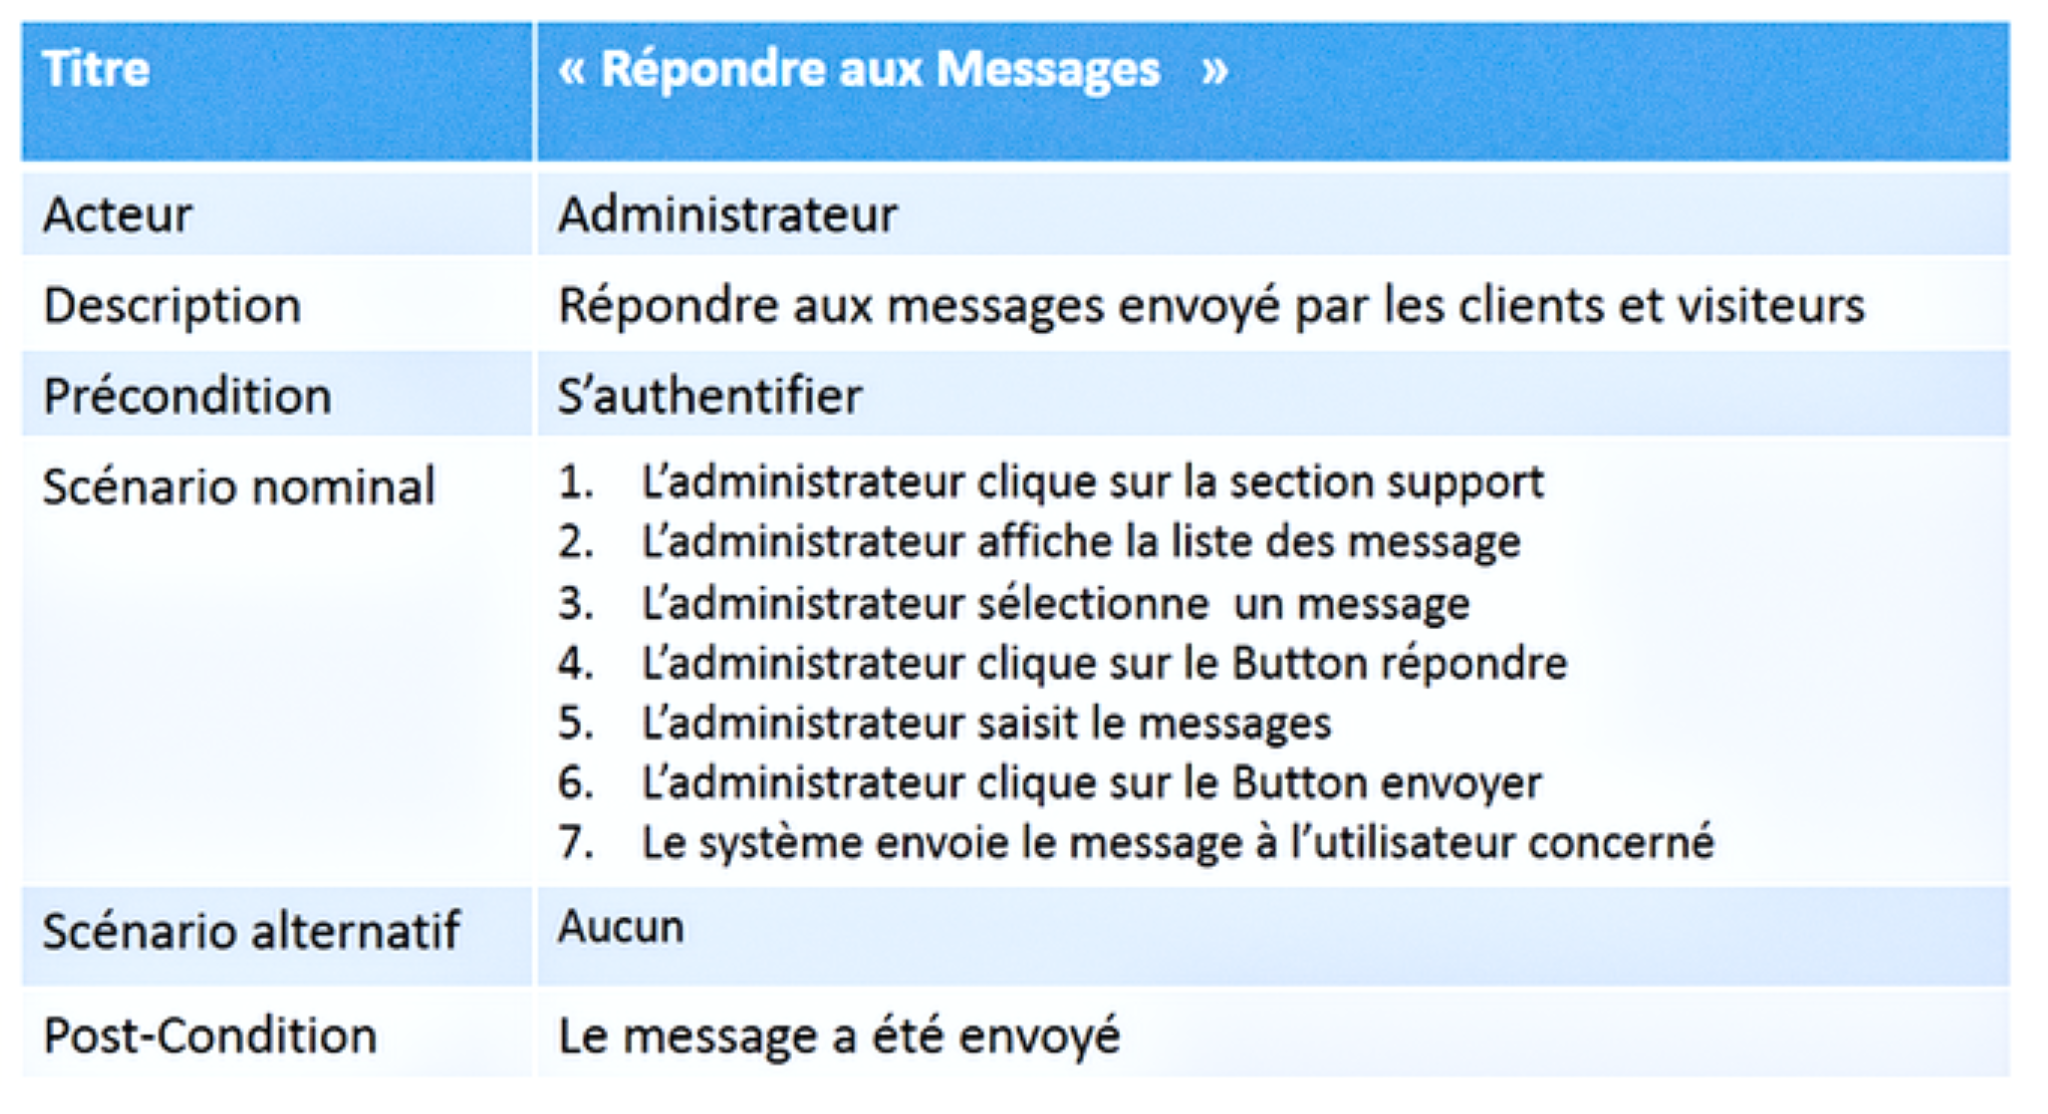
\includegraphics{img/fiche/24}
	\caption{Fiche textuelle du cas "Répondre aux Messages"}
	\label{Tux}
\end{table}
\begin{table}[H]
	\centering
	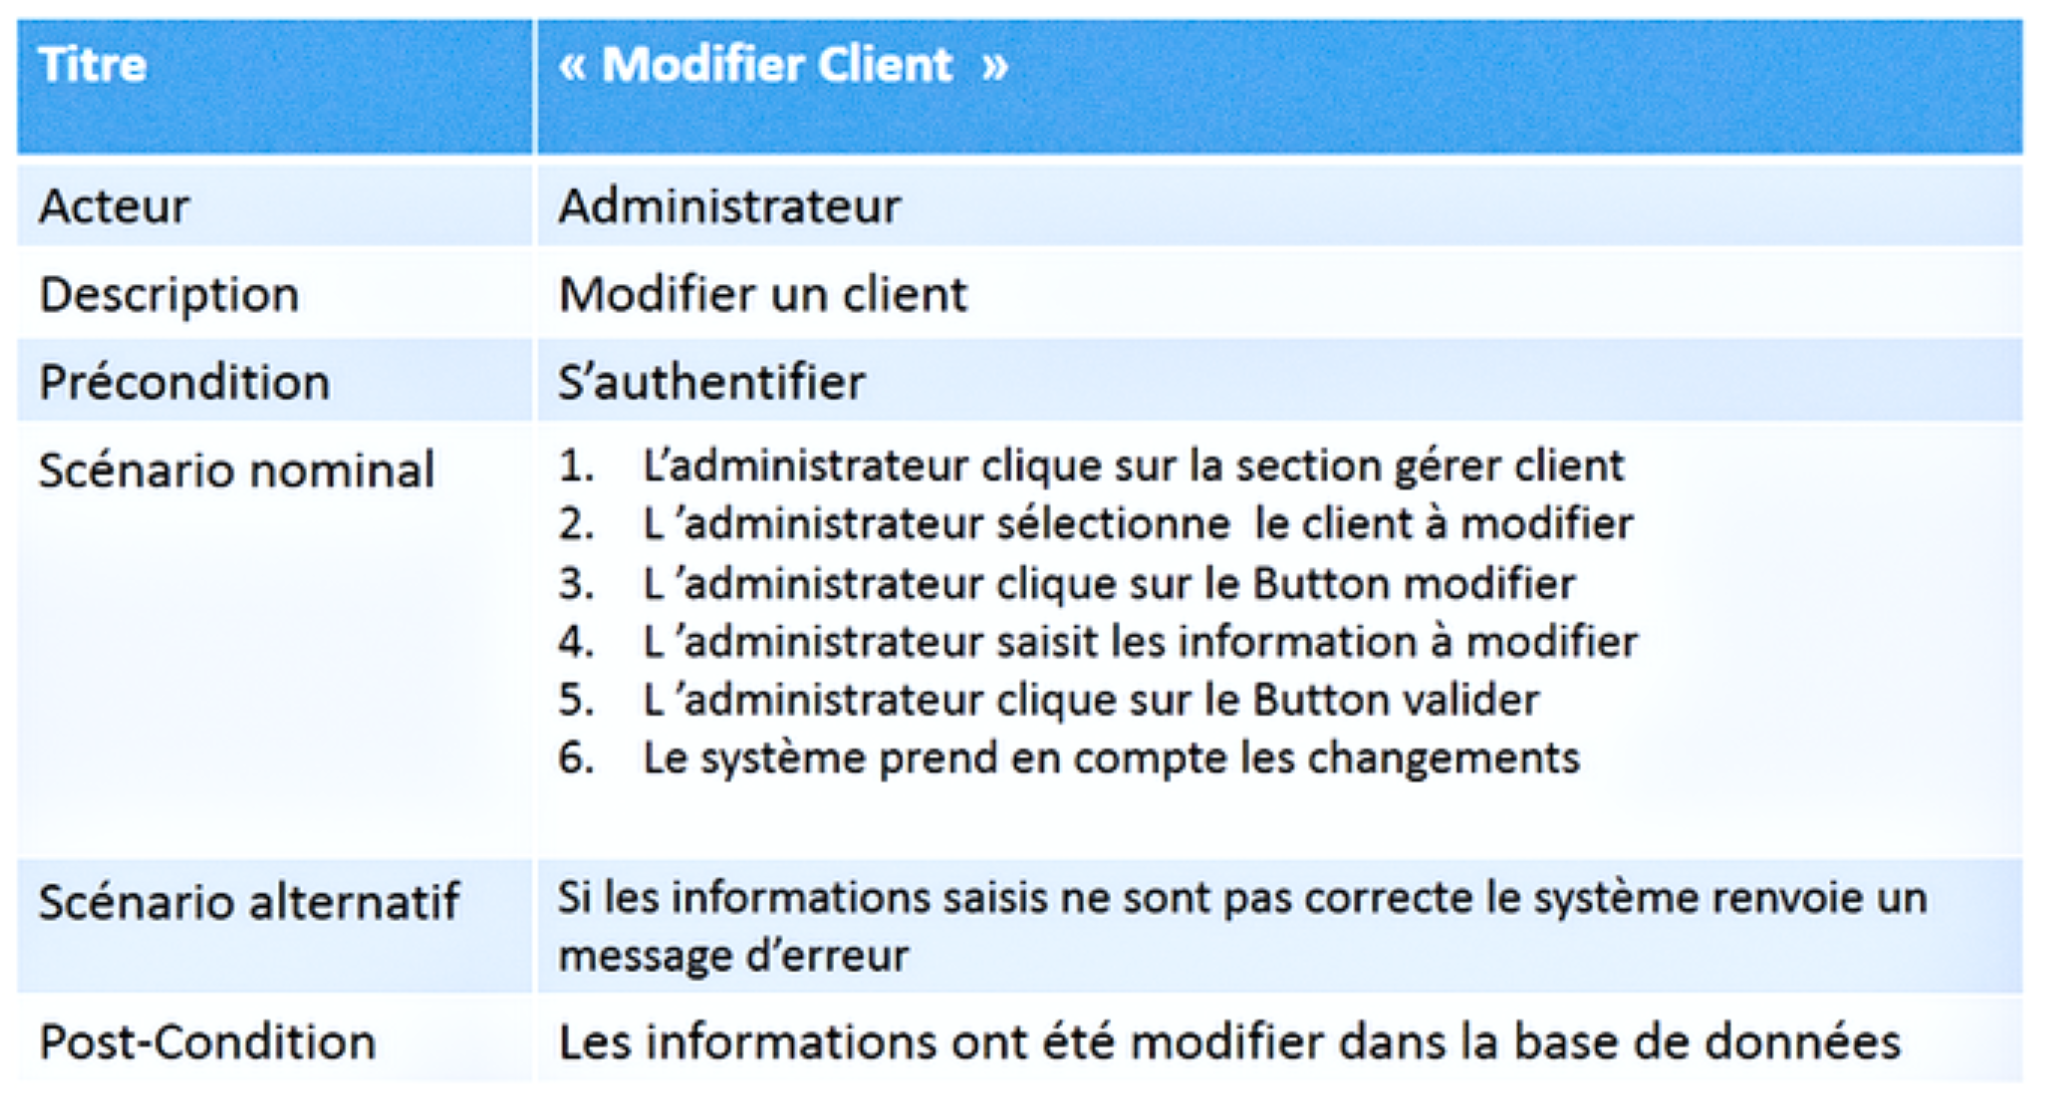
\includegraphics{img/fiche/25}
	\caption{Fiche textuelle du cas "Modifier Client"}
	\label{Tux}
\end{table}
\section{Diagramme de séquence}
\noindent Un diagramme de séquence est un document graphique qui montre pour des scenarios de cas d’utilisation précis, les évènements générés et les interactions entre objets en se basant sur des messages ordonnés. Chaque message transitant sur un lien est symbolisé par une flèche porteuse d’une expression. La lecture se fait de haut en bas, et l’ordre chronologique doit respecter ce sens ;
La réalisation du diagramme de séquence permet de lister les méthodes dont on aura besoin lors de la phase de développement. Pour se faire, la description doit être suffisamment générale et exhaustive pour identifier tous les algorithmes.
\begin{figure}[H]
	\centering
	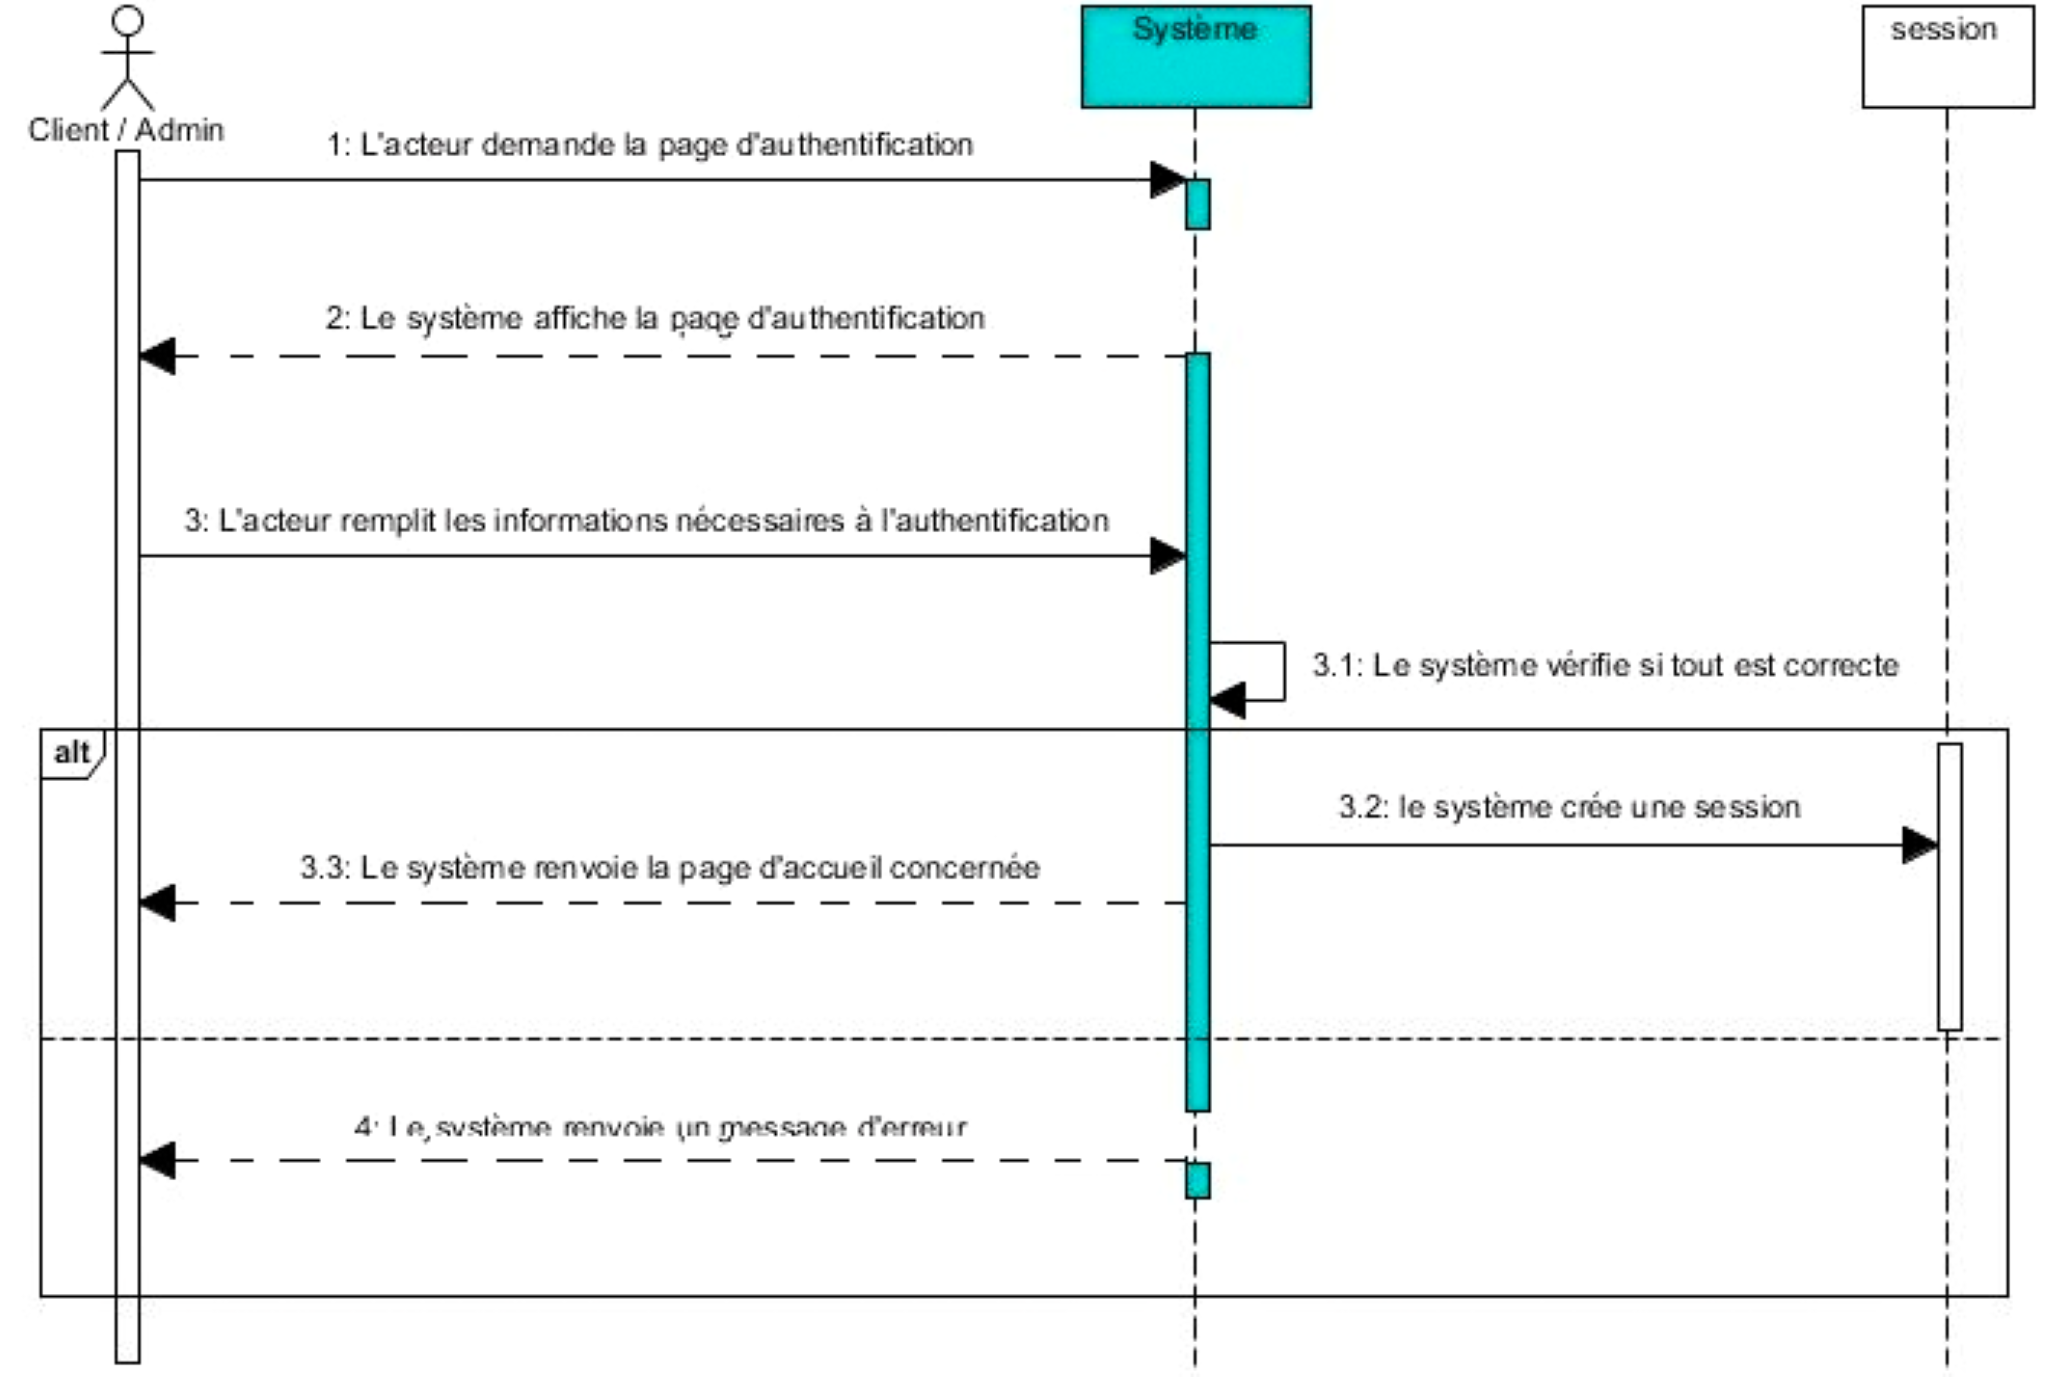
\includegraphics{img/sequence/1}
	\caption{Diagramme de séquence du cas "s'authentifier"}
	\label{Tux}
\end{figure}
\noindent Ainsi une fois qu’un utilisateur veut ouvrir son espace personnel, une page d’authentification se présente, il doit saisir son login et son mot de passe. Ensuite le système effectue une opération de vérification et affiche
Leur page personnelle, Cependant si le login et le mot de passe sont incorrects le système envoie un message d’erreur   

\begin{figure}[H]
	\centering
	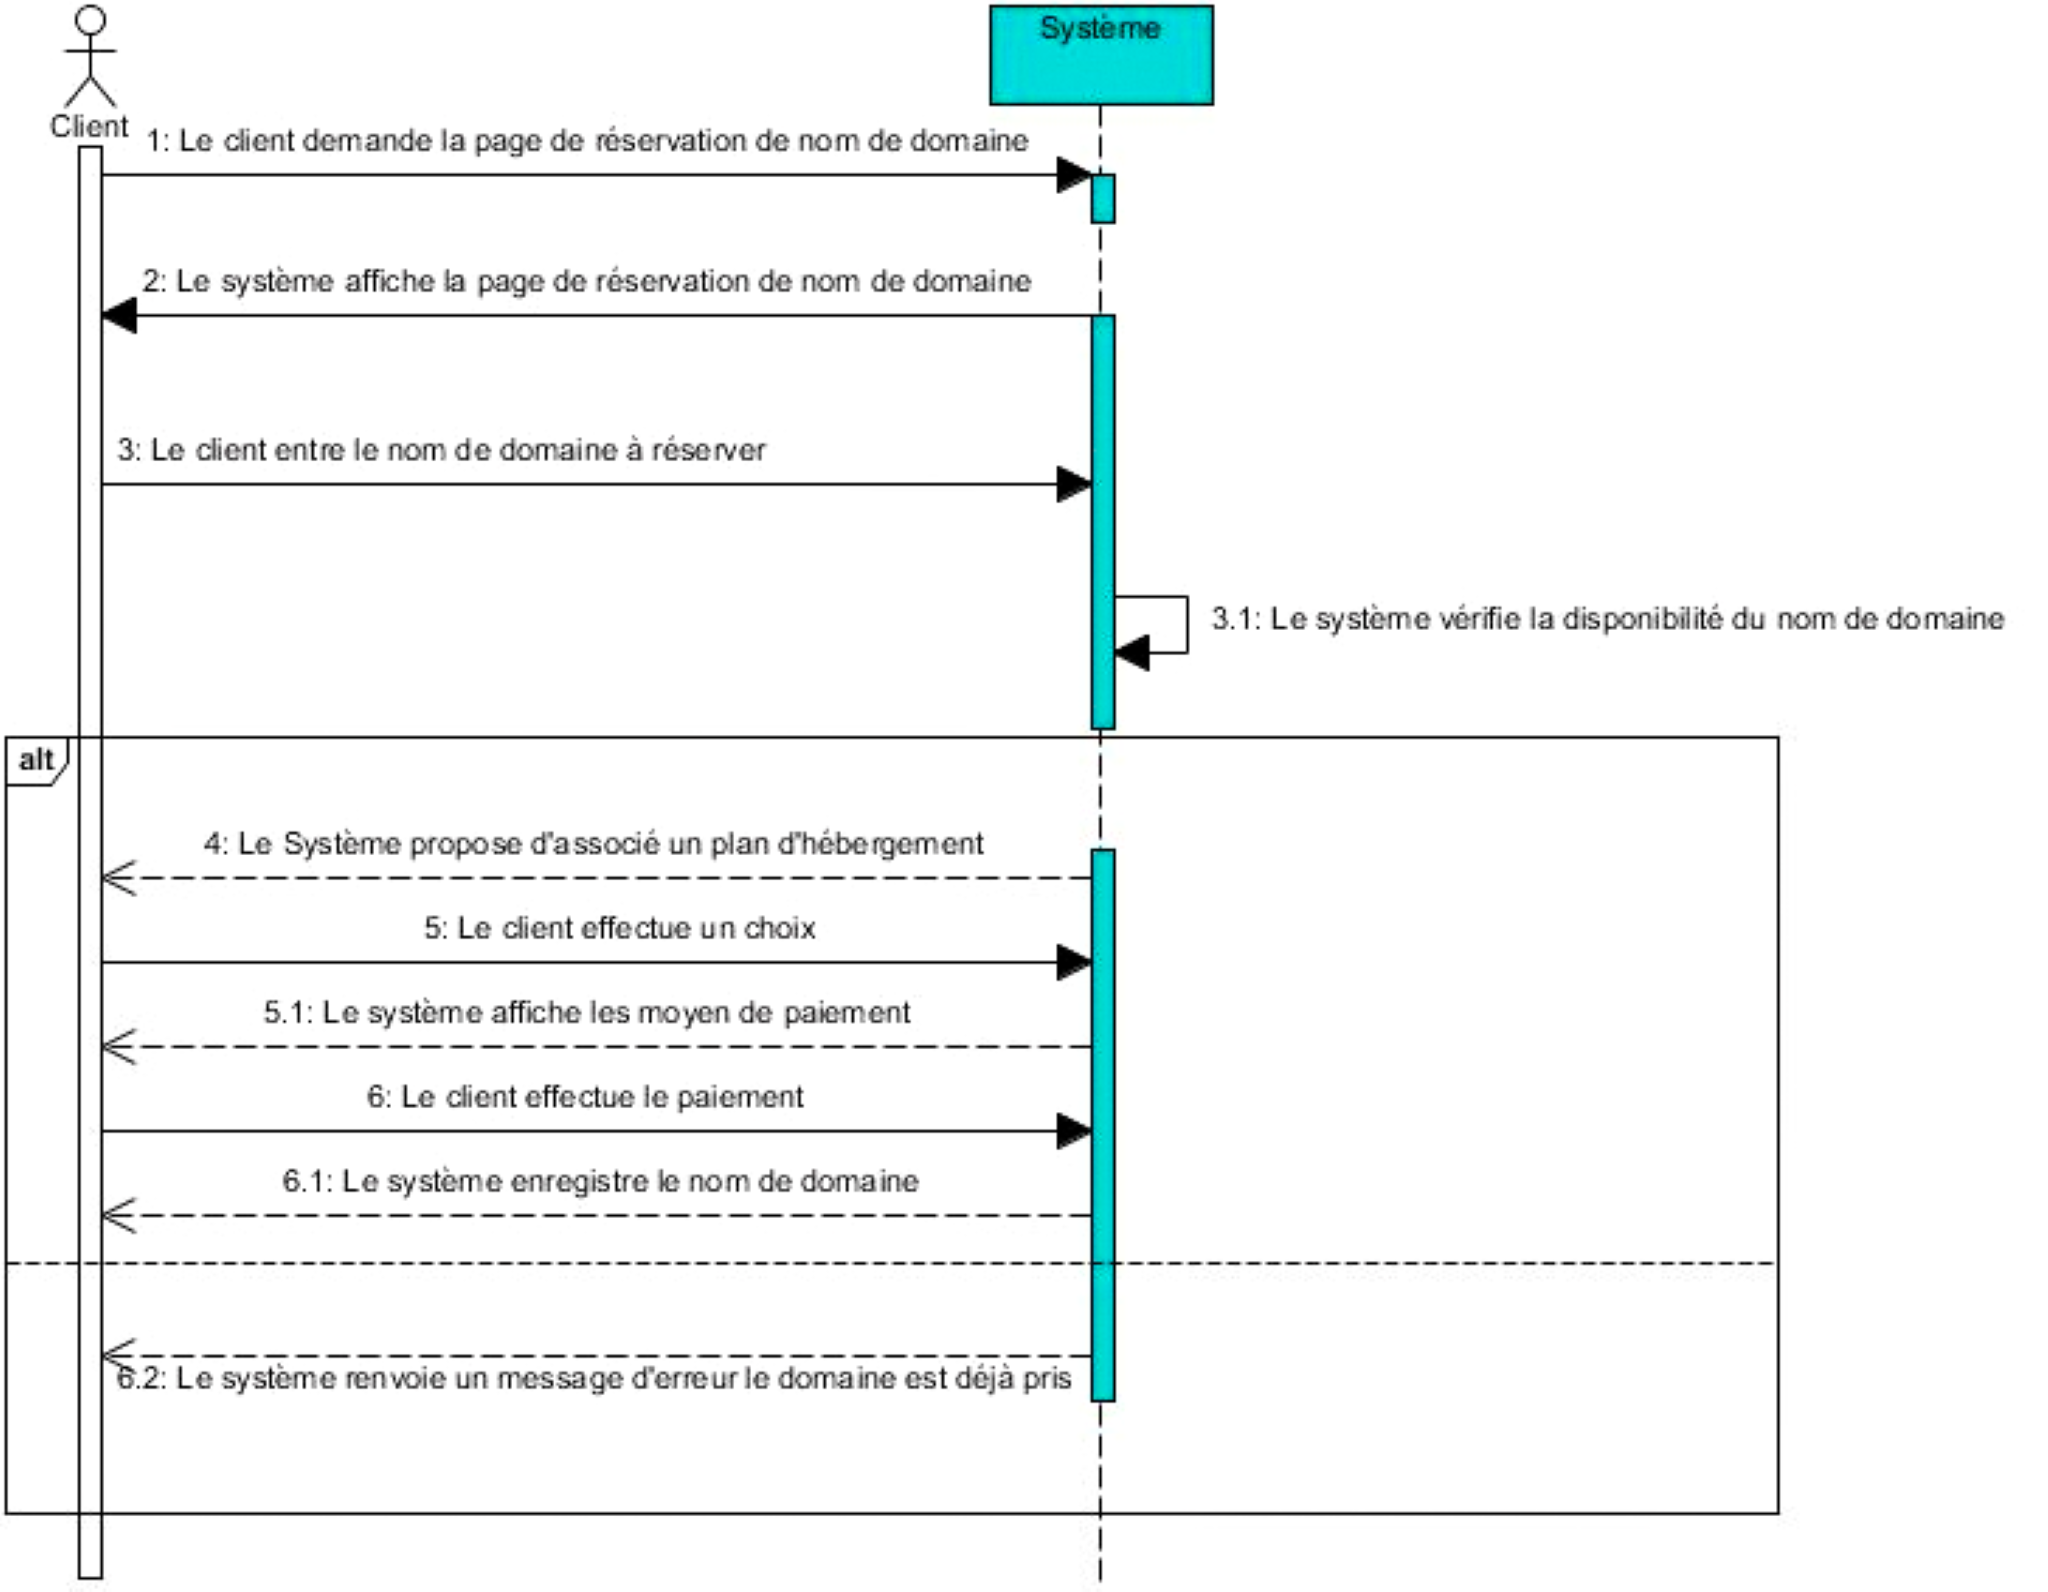
\includegraphics{img/sequence/2}
	\caption{Diagramme de séquence du cas "Réserver un nom de domaine}
	\label{Tux}
\end{figure}
\noindent Lorsqu’un client veut réserver un nom de domaine, il peut cliquer sur le bouton « Domaine » qui est dans le menu principal ensuite il peut saisir le nom ainsi que le tld,, valider sa saisie et procédé au mode de paiement .Une fois que le client achève le paiement , le système effectue une opération de vérification et enregistre le nom de domaine
\begin{figure}[H]
	\centering
	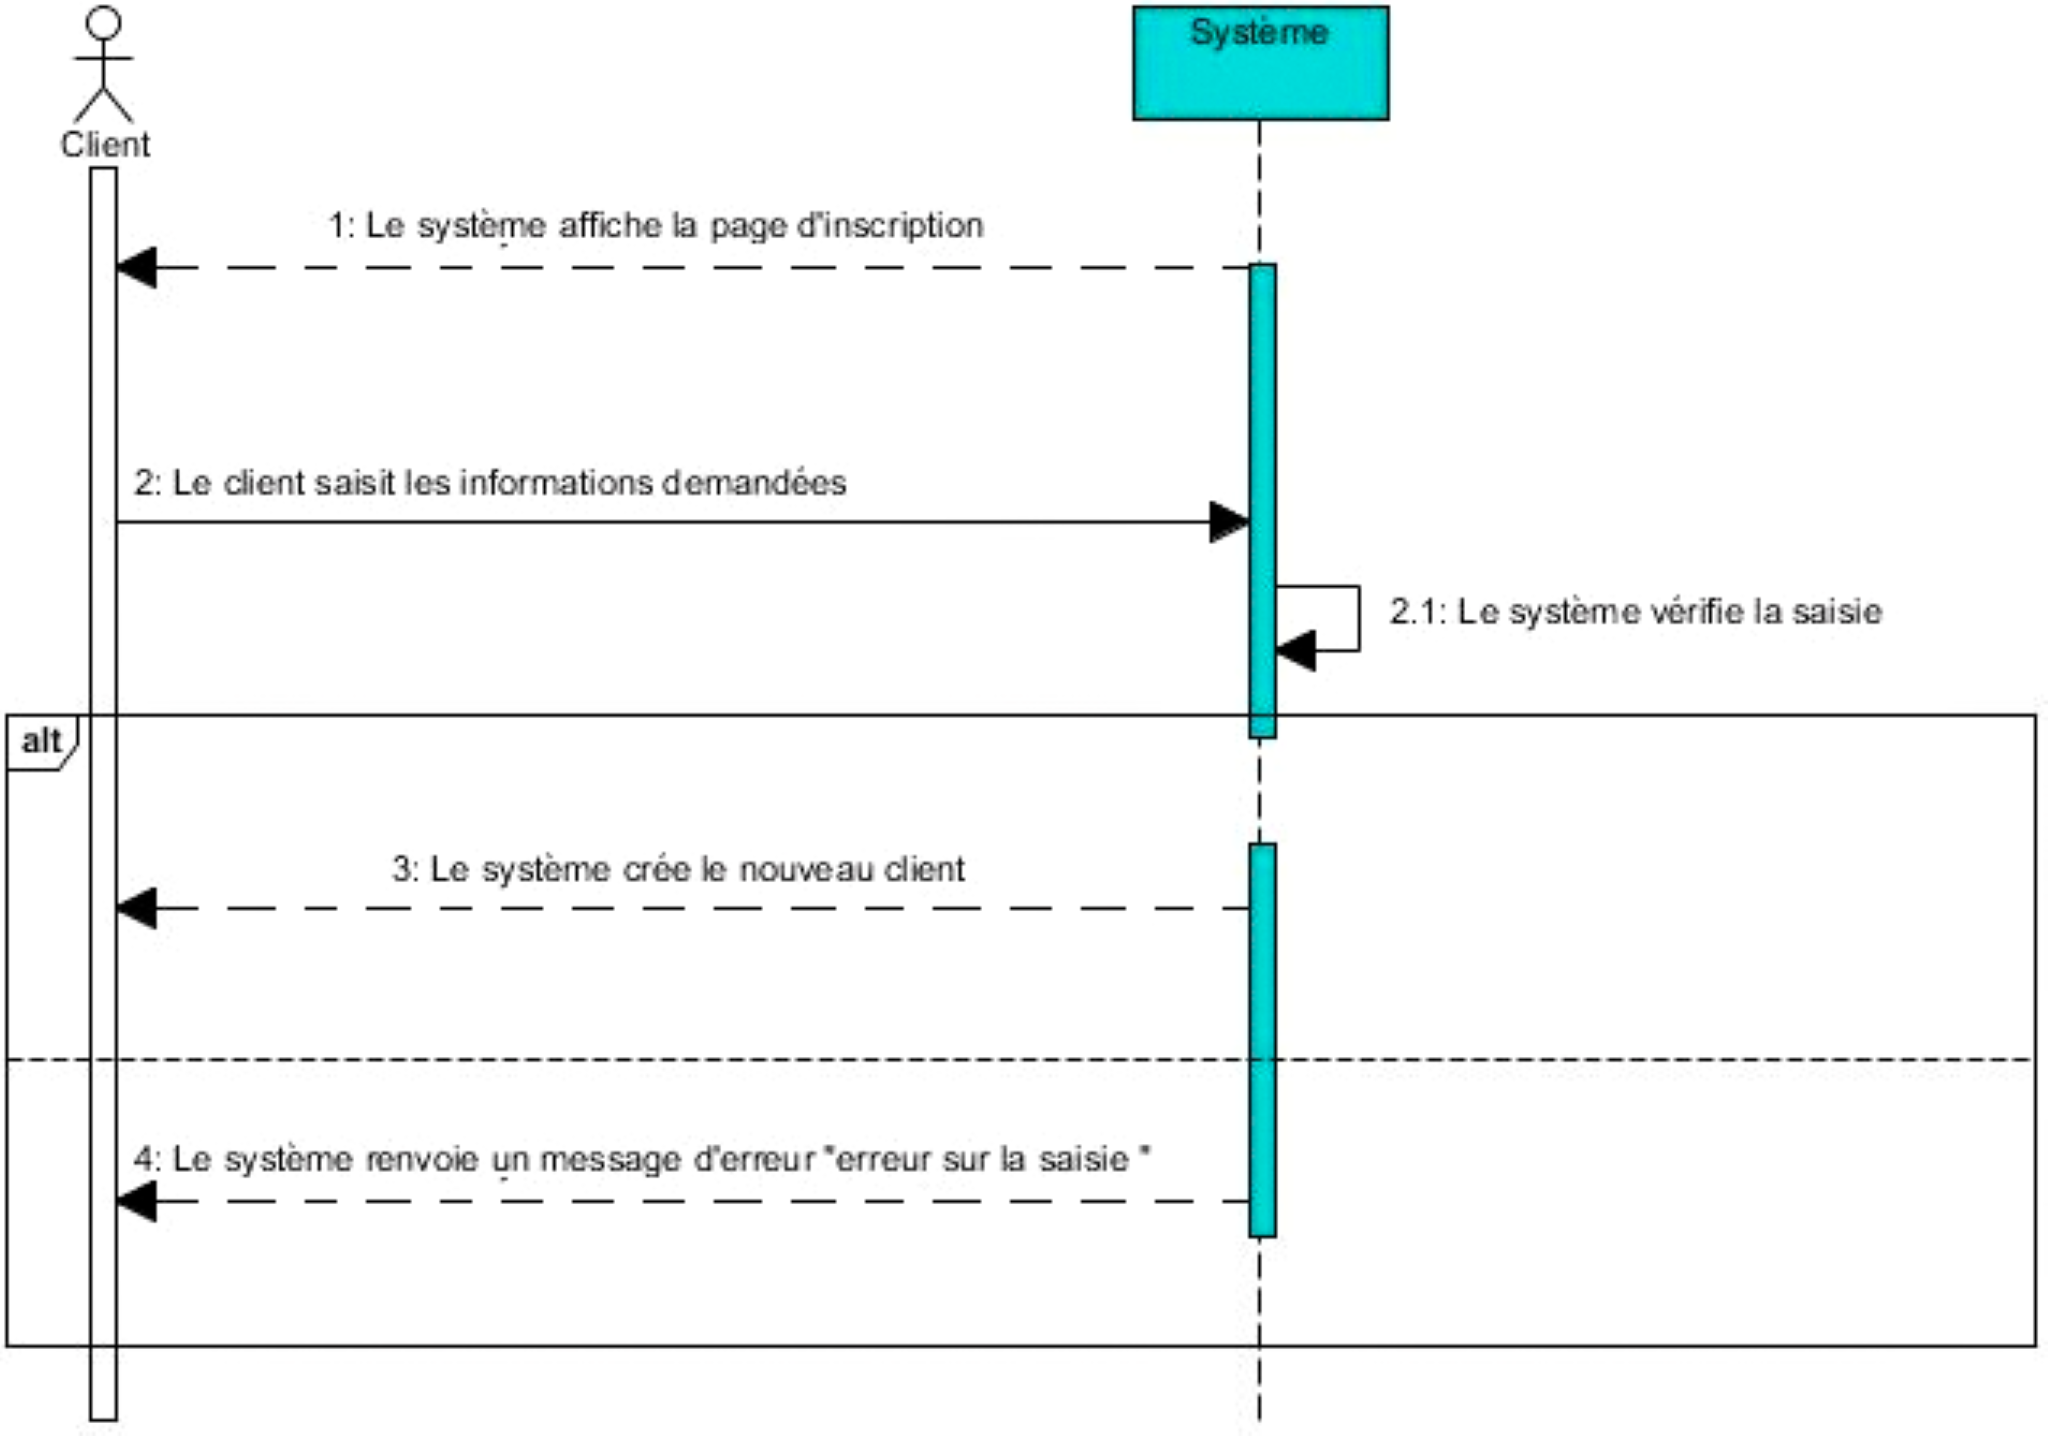
\includegraphics{img/sequence/3}
	\caption{Diagramme de séquence du cas "S’inscrire}
	\label{Tux}
\end{figure}
\noindent Le visiteur peut devenir client ou administrateur uniquement s’il s’inscrit en remplissant les champs 
Le système va générer un nom d’utilisateur et un mot de passe qu’il va utiliser a chaque fois qu’il se connecte au système  
\begin{figure}[H]
	\centering
	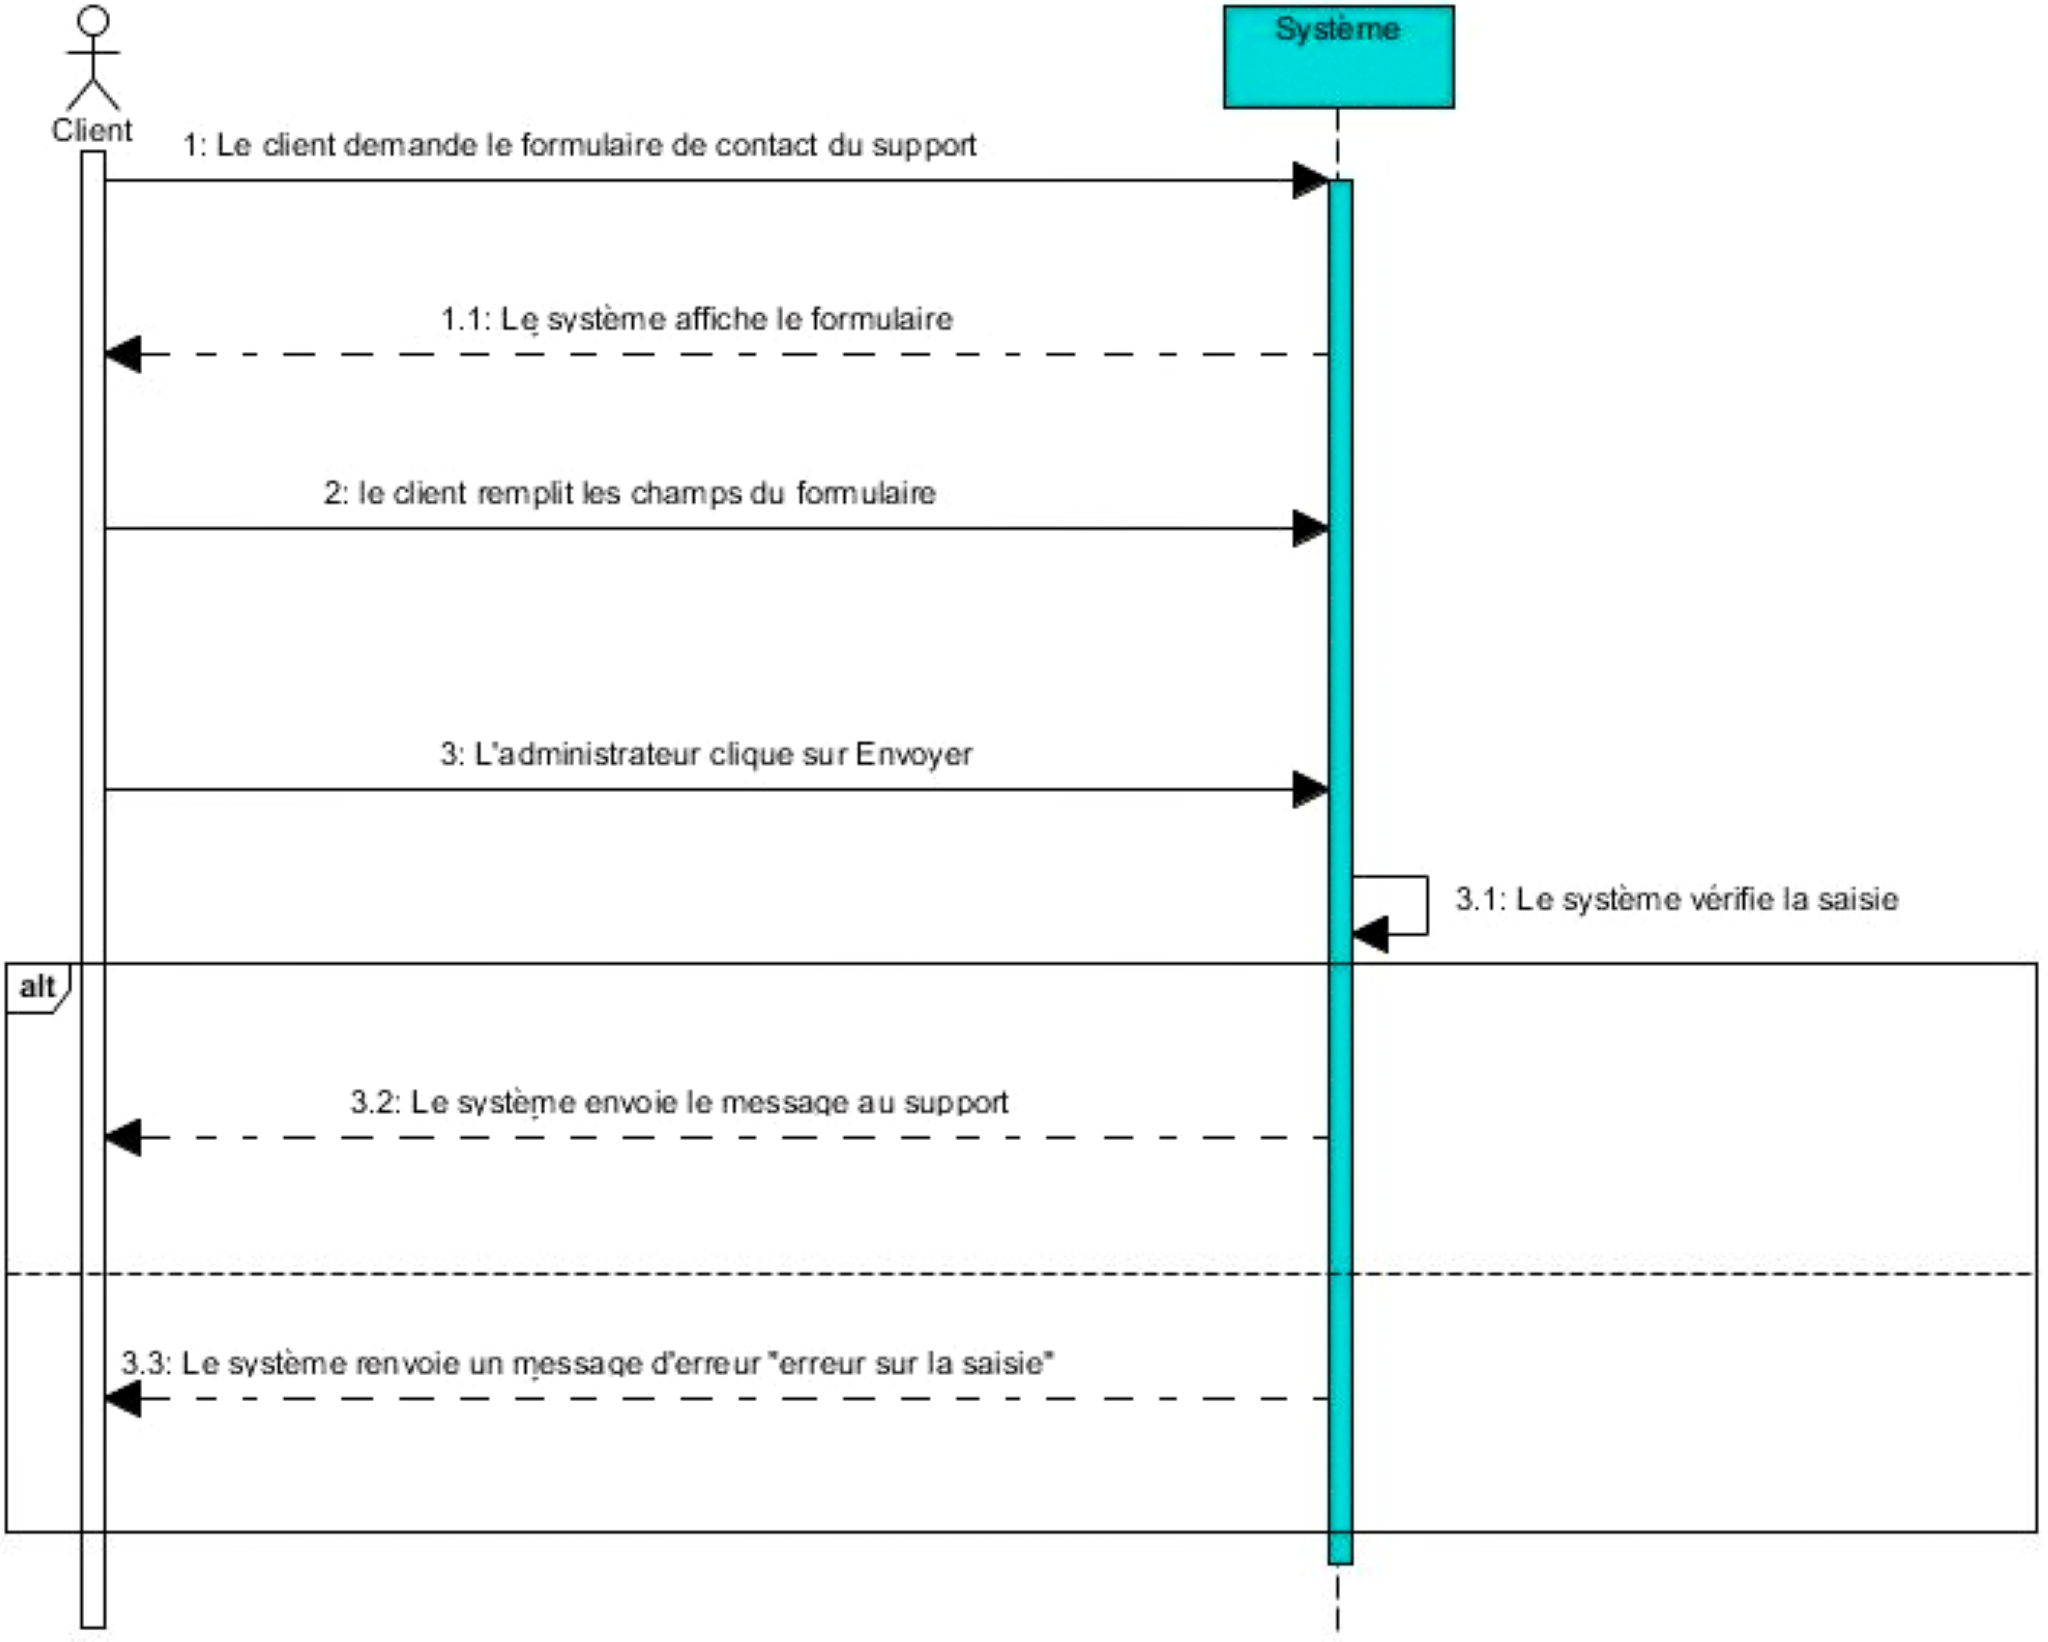
\includegraphics{img/sequence/4}
	\caption{Diagramme de séquence du cas "contacter support}
	\label{Tux}
\end{figure}
\noindent Pour contacter le support technique le client sélectionne sur le menu principal le rubrique ‘support’ ensuite il remplit le formulaire de contact. Et clique sur le bouton « Envoyer » le système envoie le message au destinataire s’il y’a des erreurs sur la saisie le système envoie un message d’erreur.   
\begin{figure}[H]
	\centering
	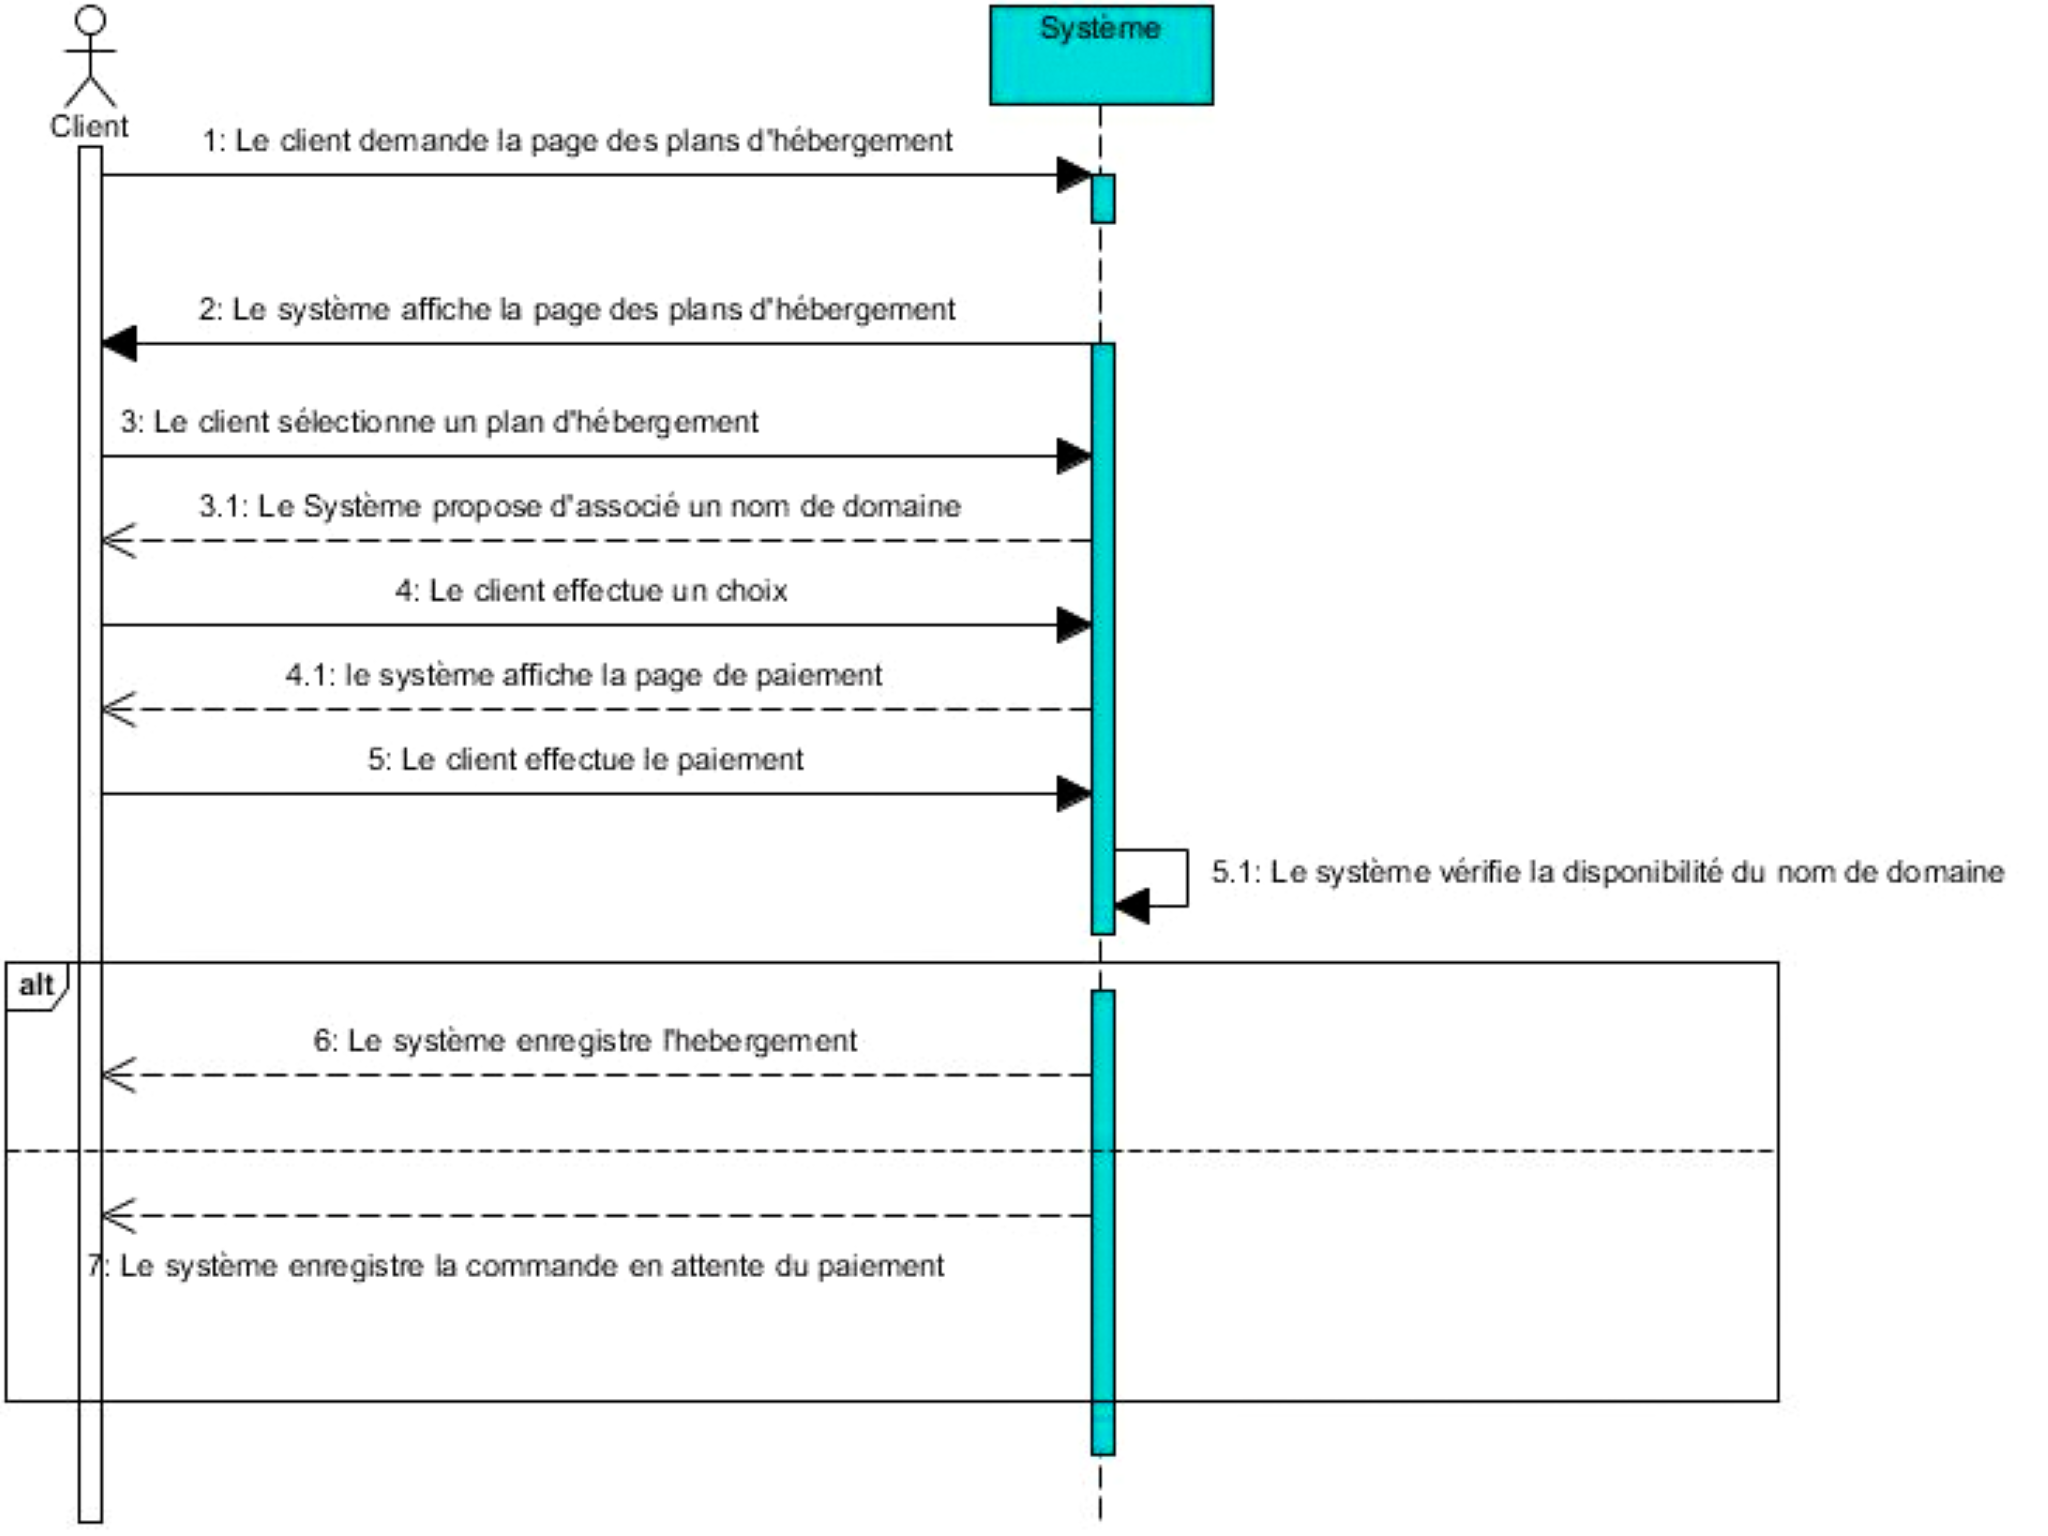
\includegraphics{img/sequence/5}
	\caption{Diagramme de séquence du cas prendre un hébergement web"}
	\label{Tux}
\end{figure}
\noindent Pour prendre un hébergement web, le client commence d’abord par sélectionner le nom de domaine concerné ensuite il sélectionne un plan d’hébergement et procède au paiement le système vérifie si tout est correcte et associe ainsi le plan d’hébergement choisi au nom de domaine 
\begin{figure}[H]
	\centering
	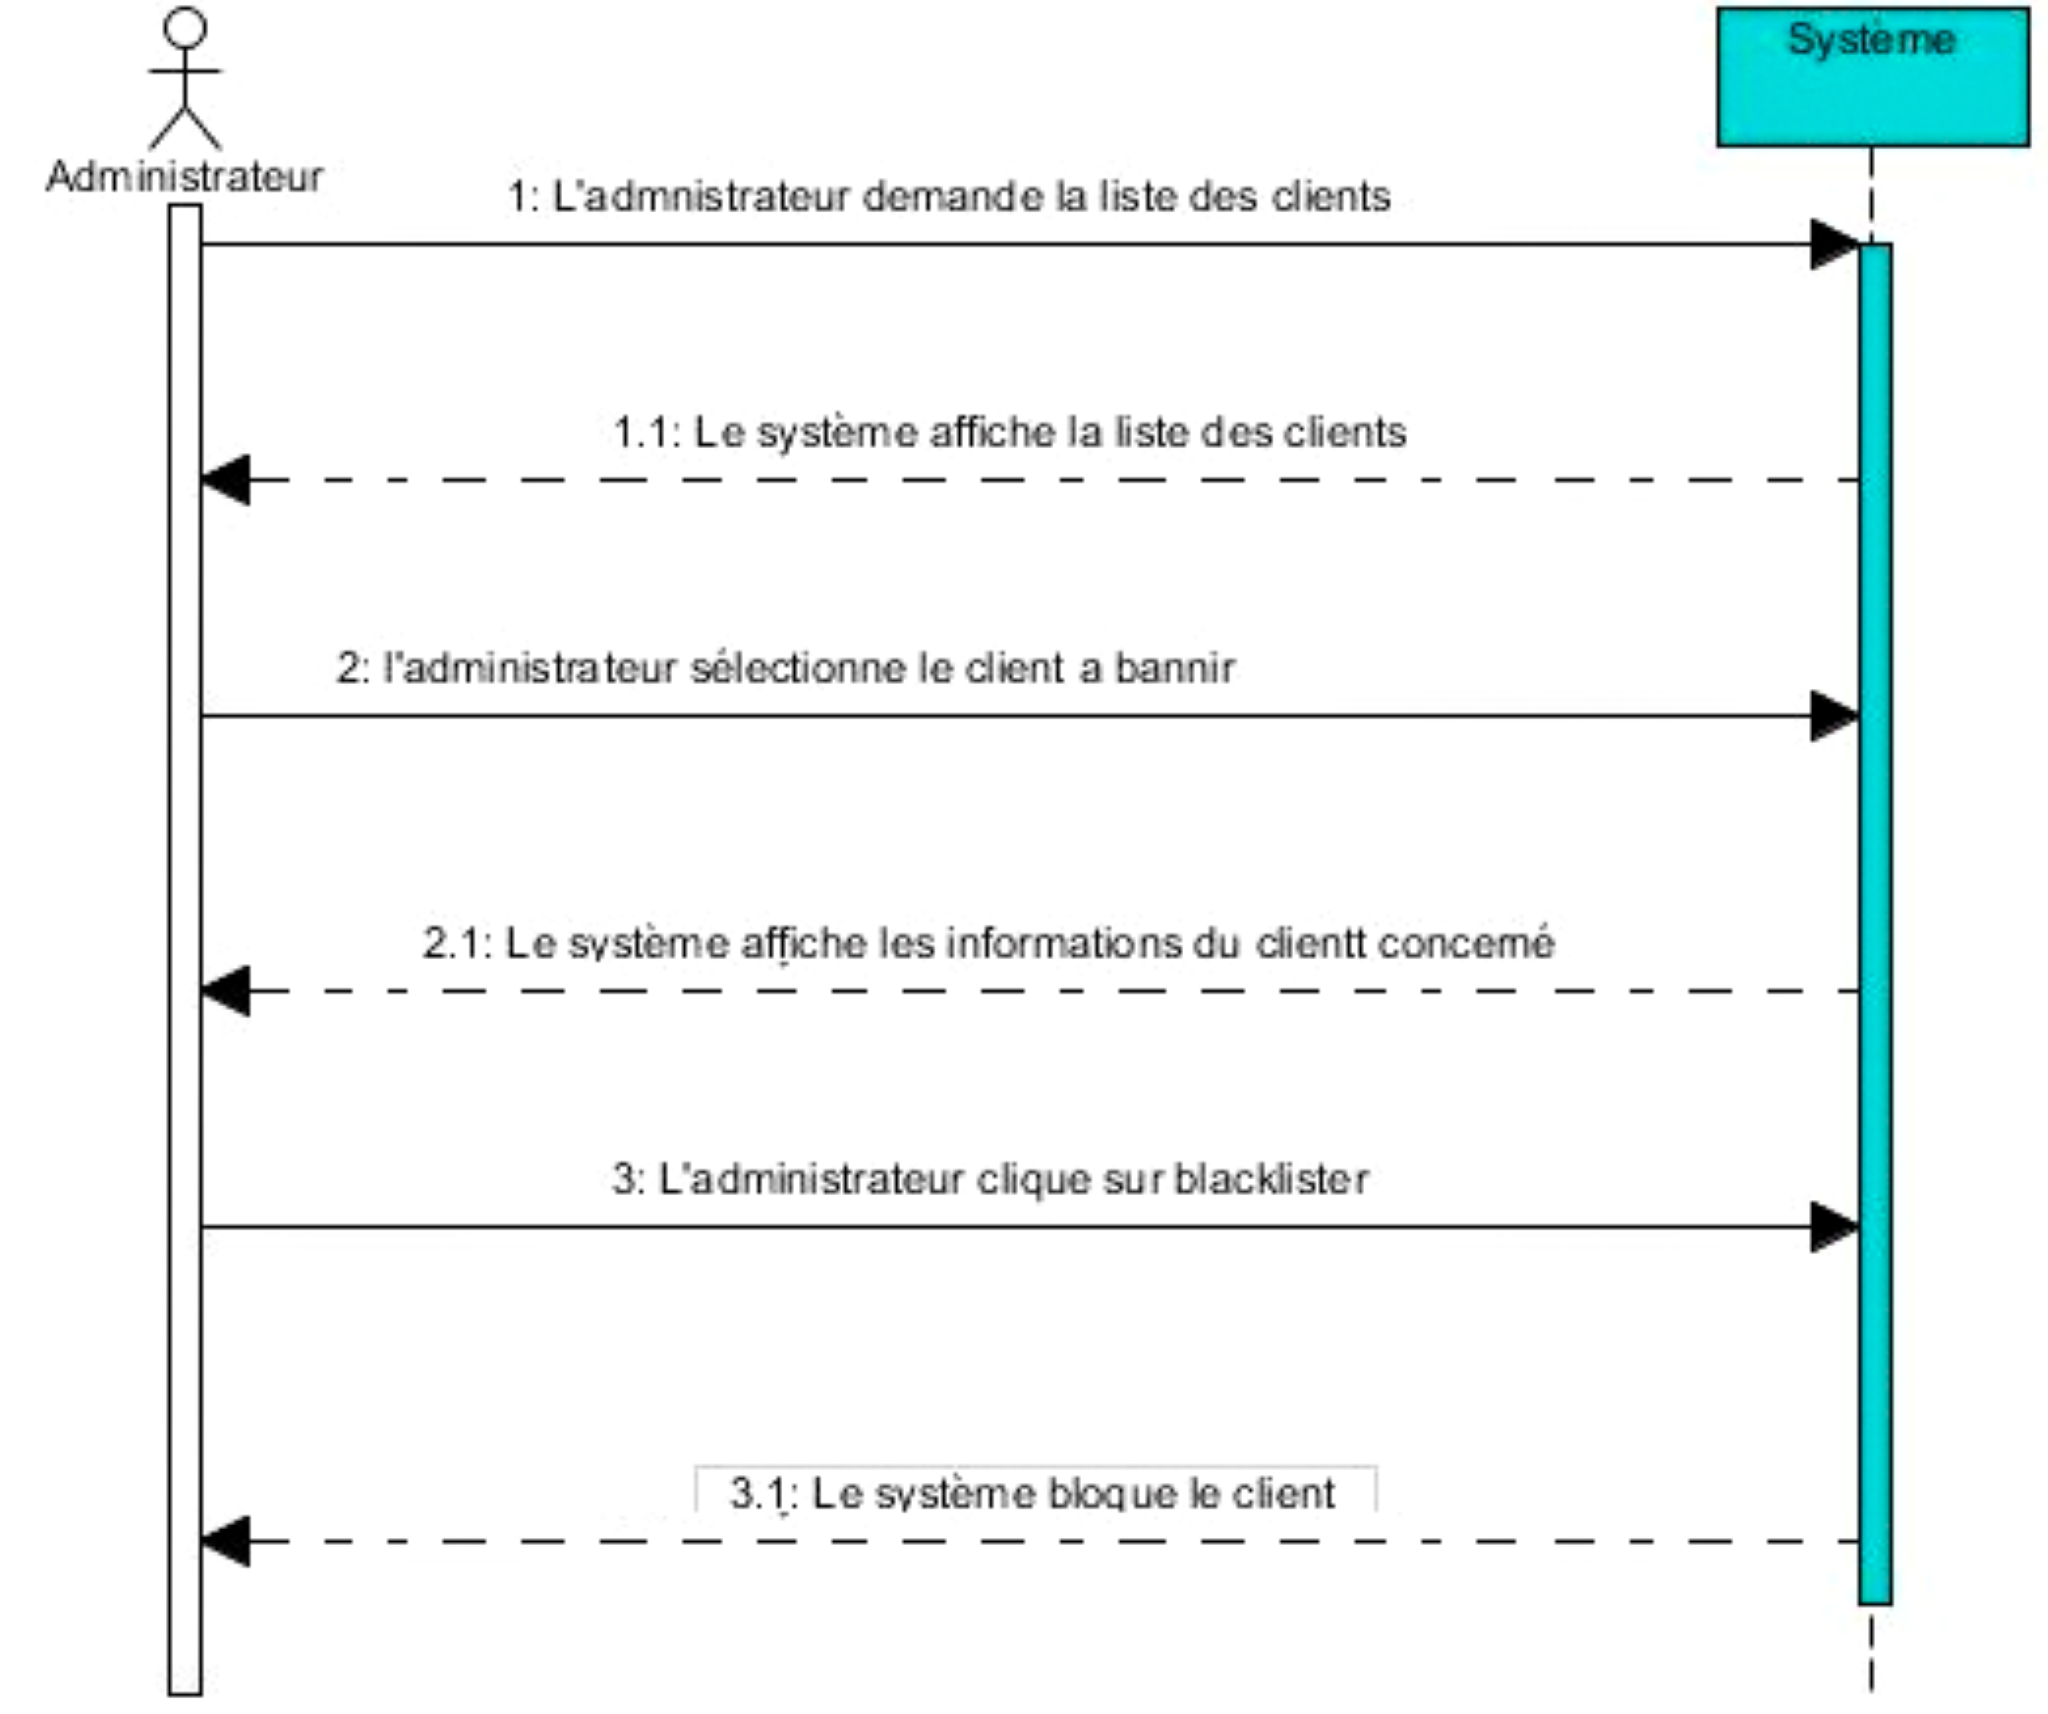
\includegraphics{img/sequence/6}
	\caption{Diagramme de séquence du cas "bannir client}
	\label{Tux}
\end{figure}
\noindent Pour bannir un client du système pour des raisons de non-respect du règlement l’administrateur devrait commencer par afficher la liste de tous les clients existants ensuite il sélectionne le client à bannir puis cliquer sur le bouton bannir 
Ainsi le système bannit le client 

\begin{figure}[H]
	\centering
	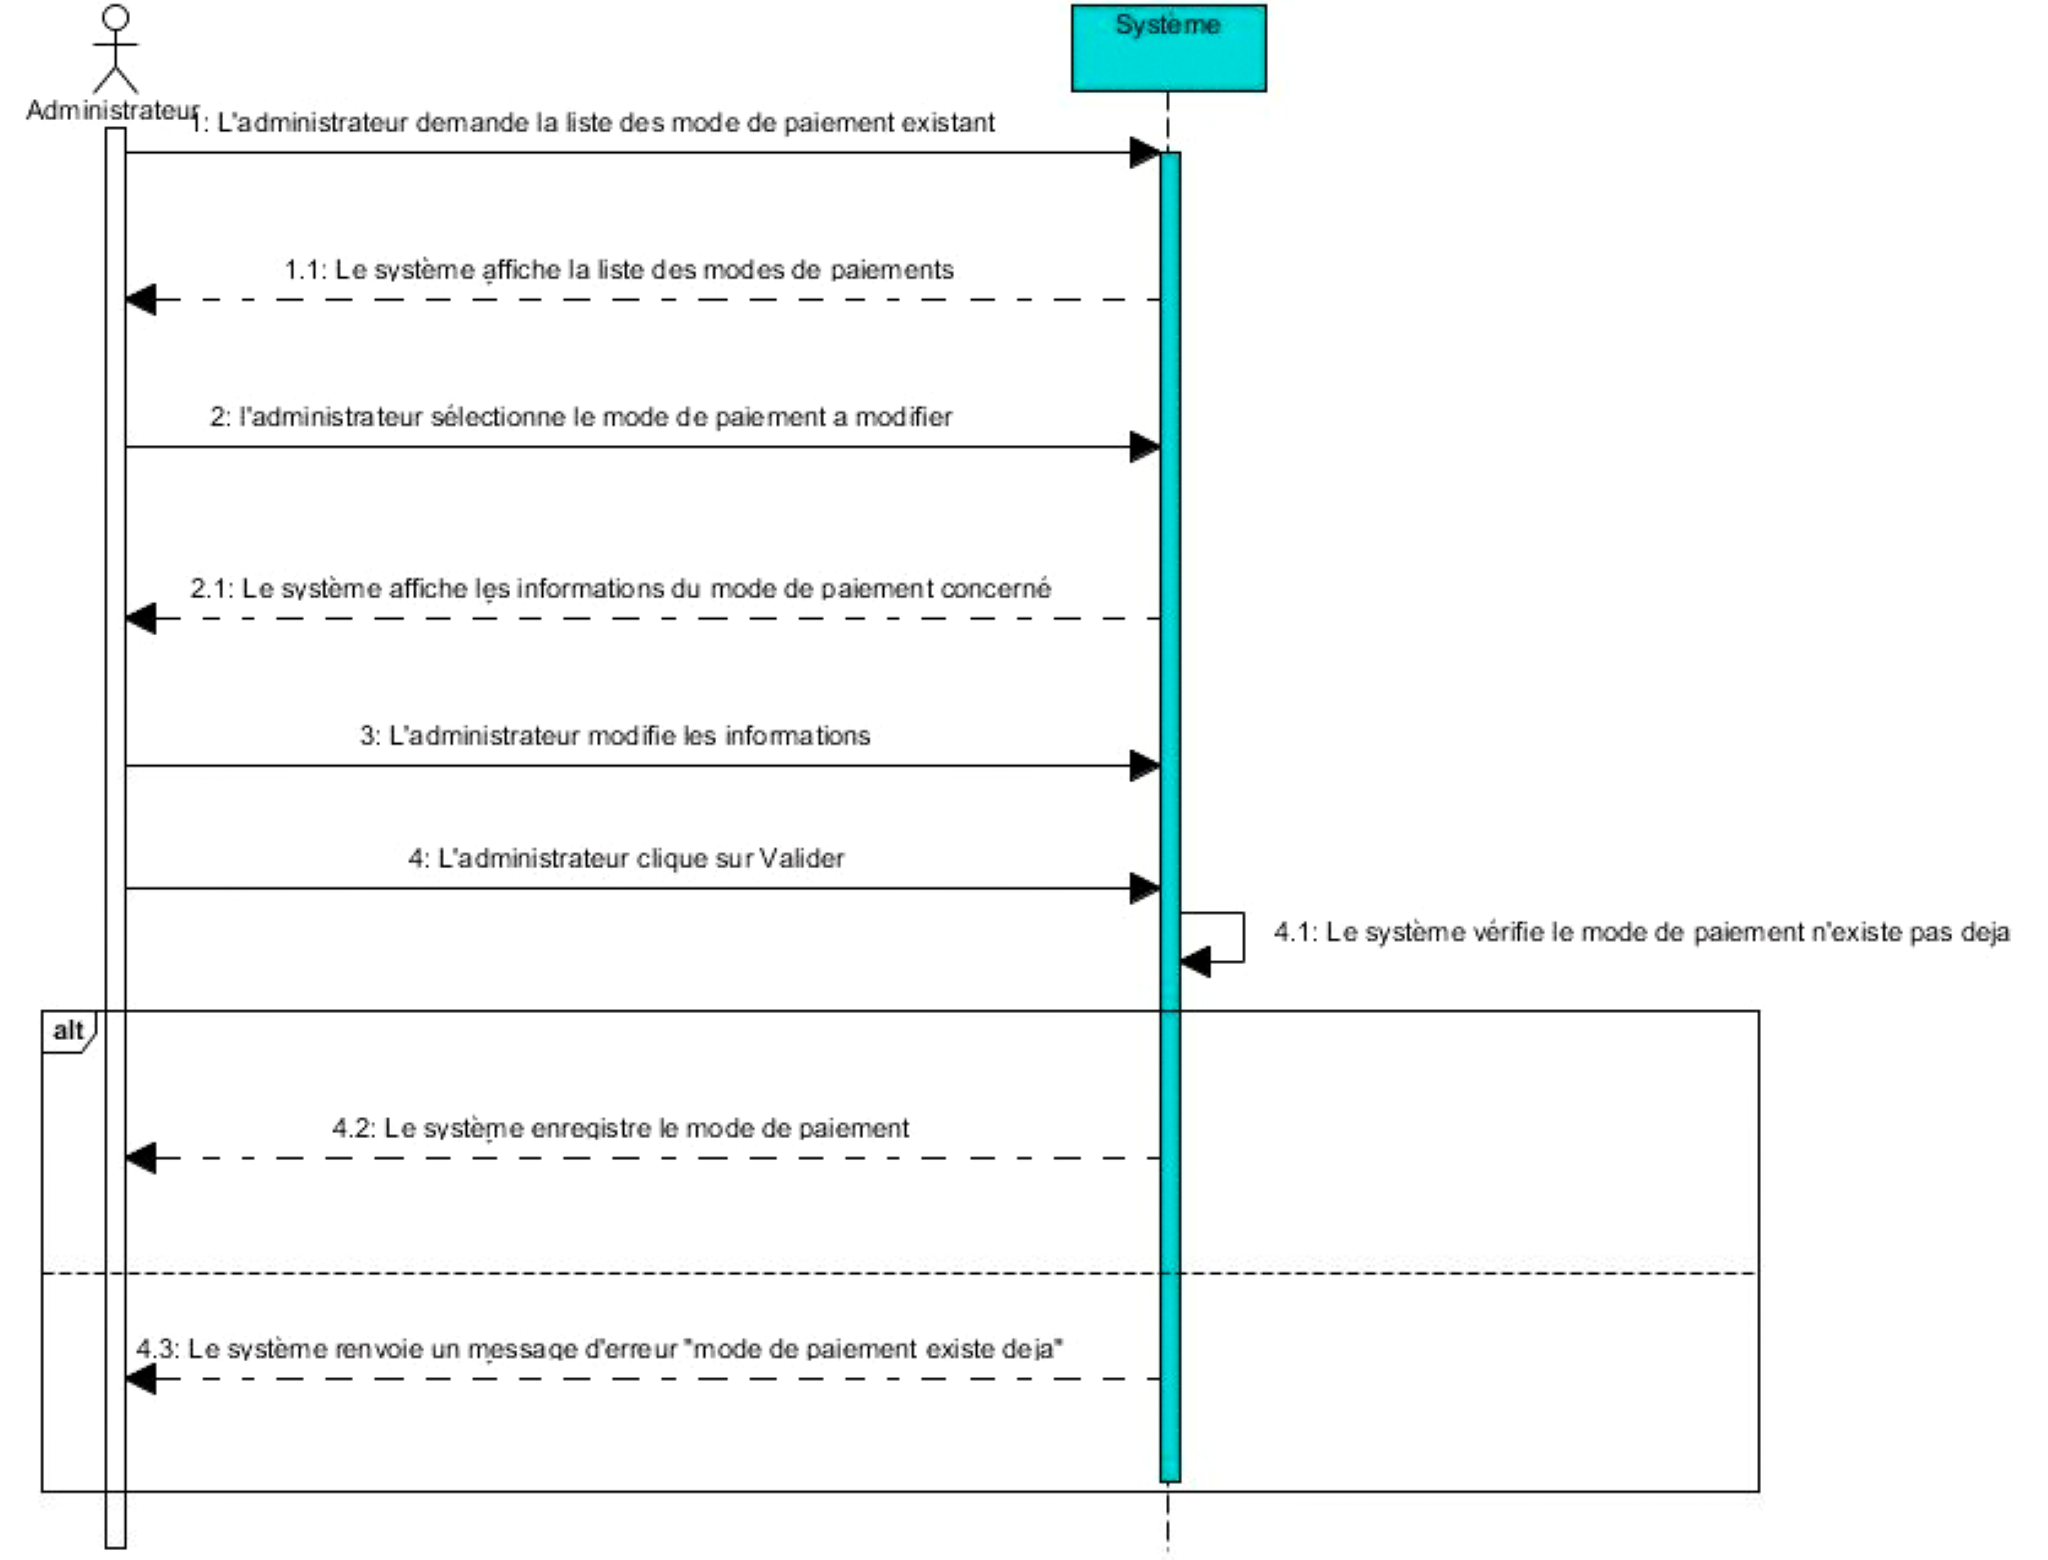
\includegraphics{img/sequence/7}
	\caption{Diagramme de séquence du cas "ajouter un mode de paiement}
	\label{Tux}
\end{figure}
\noindent Pour ajouter un nouveau mode de paiement l’administrateur devra aller sur l’onglet paiement ensuite il clique sur le bouton ajouter un nouveau mode de paiement, il remplit le formulaire et clique sur le bouton valider
Le système enregistre le mode de paiement s’il y’a des erreurs sur la saisie le système envoie un message d’erreur.   

\section{Diagramme de classe}
\begin{figure}[H]
	\centering
	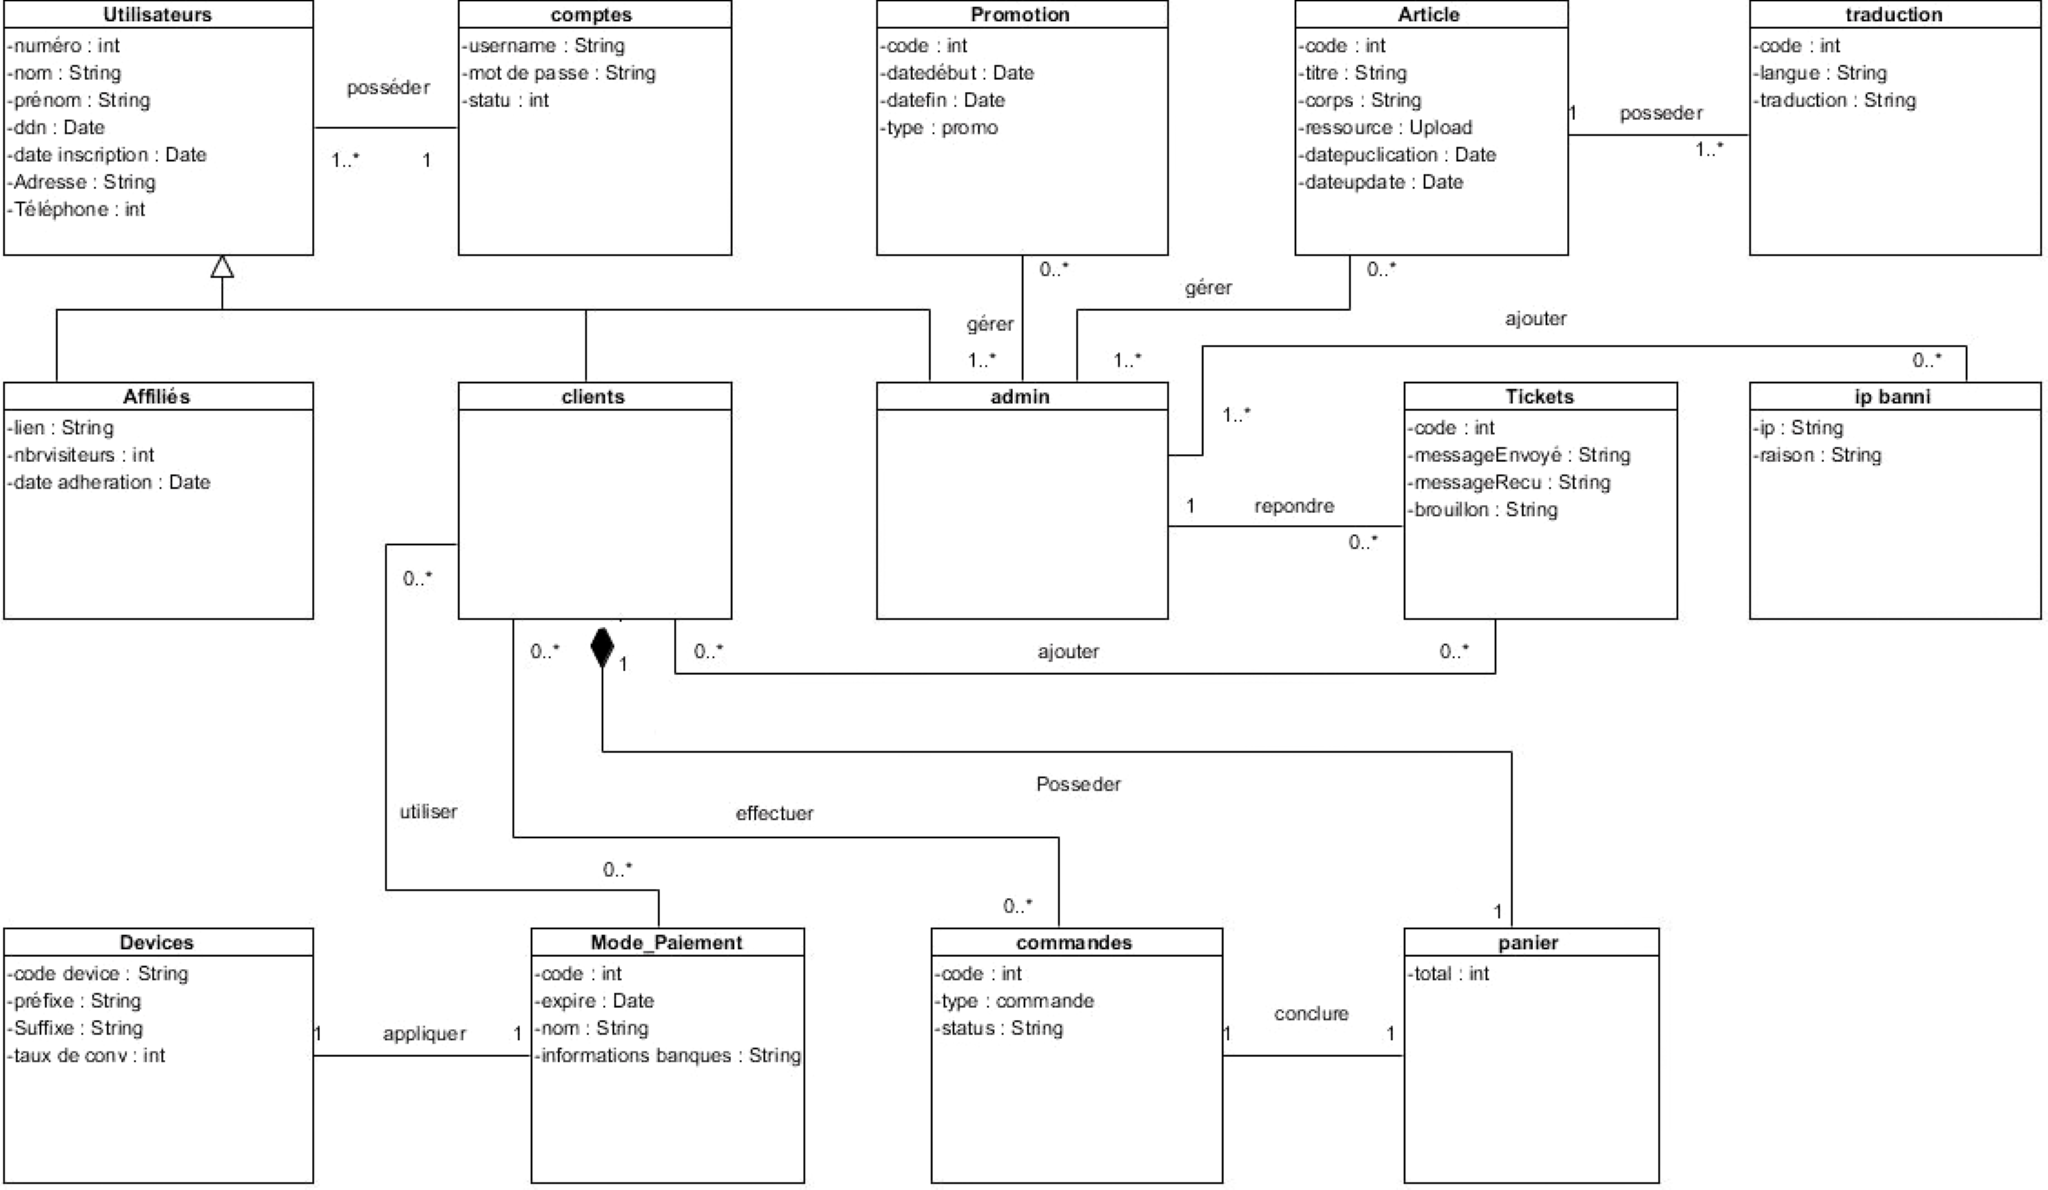
\includegraphics{img/diagclasse/1}
	\caption{Diagramme de Classe d’Analyse (1/2)}
	\label{Tux}
\end{figure}
\begin{figure}[H]
	\centering
	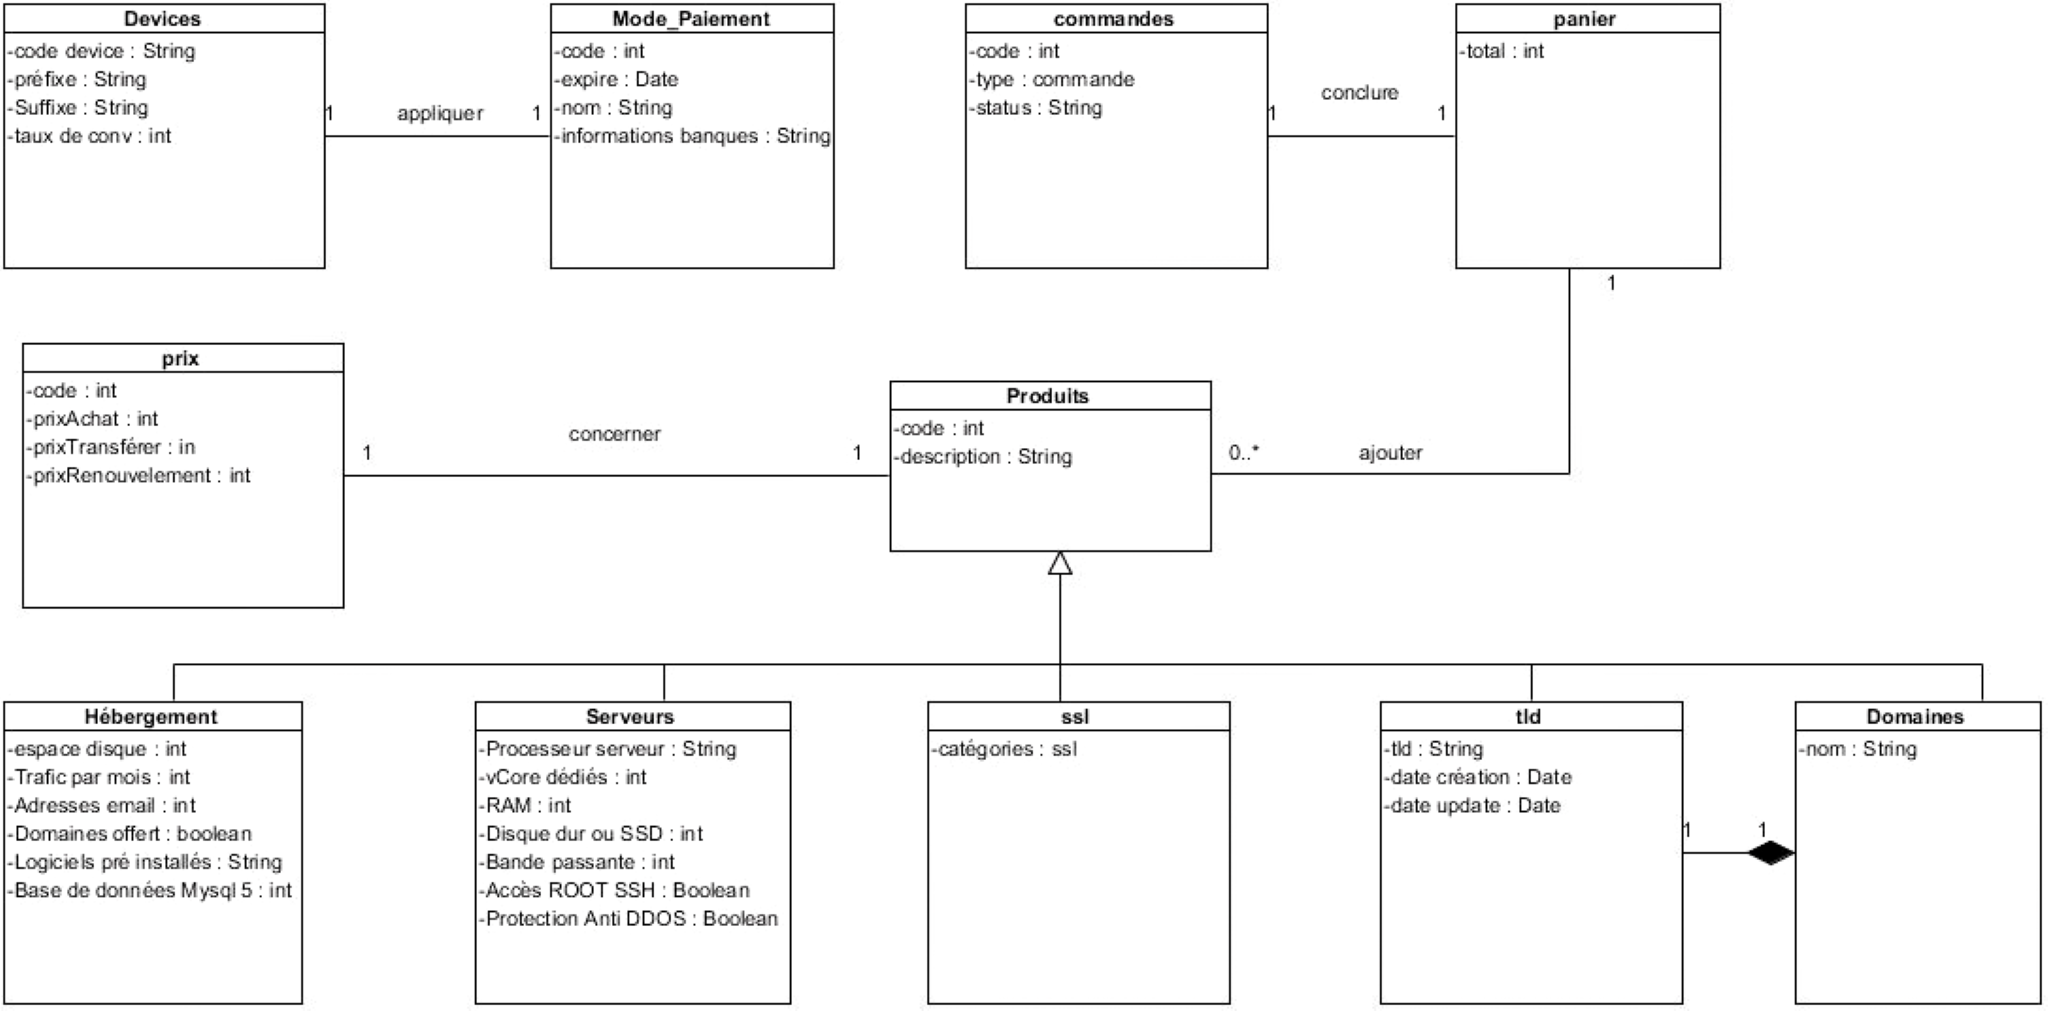
\includegraphics{img/diagclasse/2}
	\caption{Diagramme de Classe d’Analyse (2/2)}
		\label{Tux}
\end{figure}
	\begin{figure}[H]
		\centering
		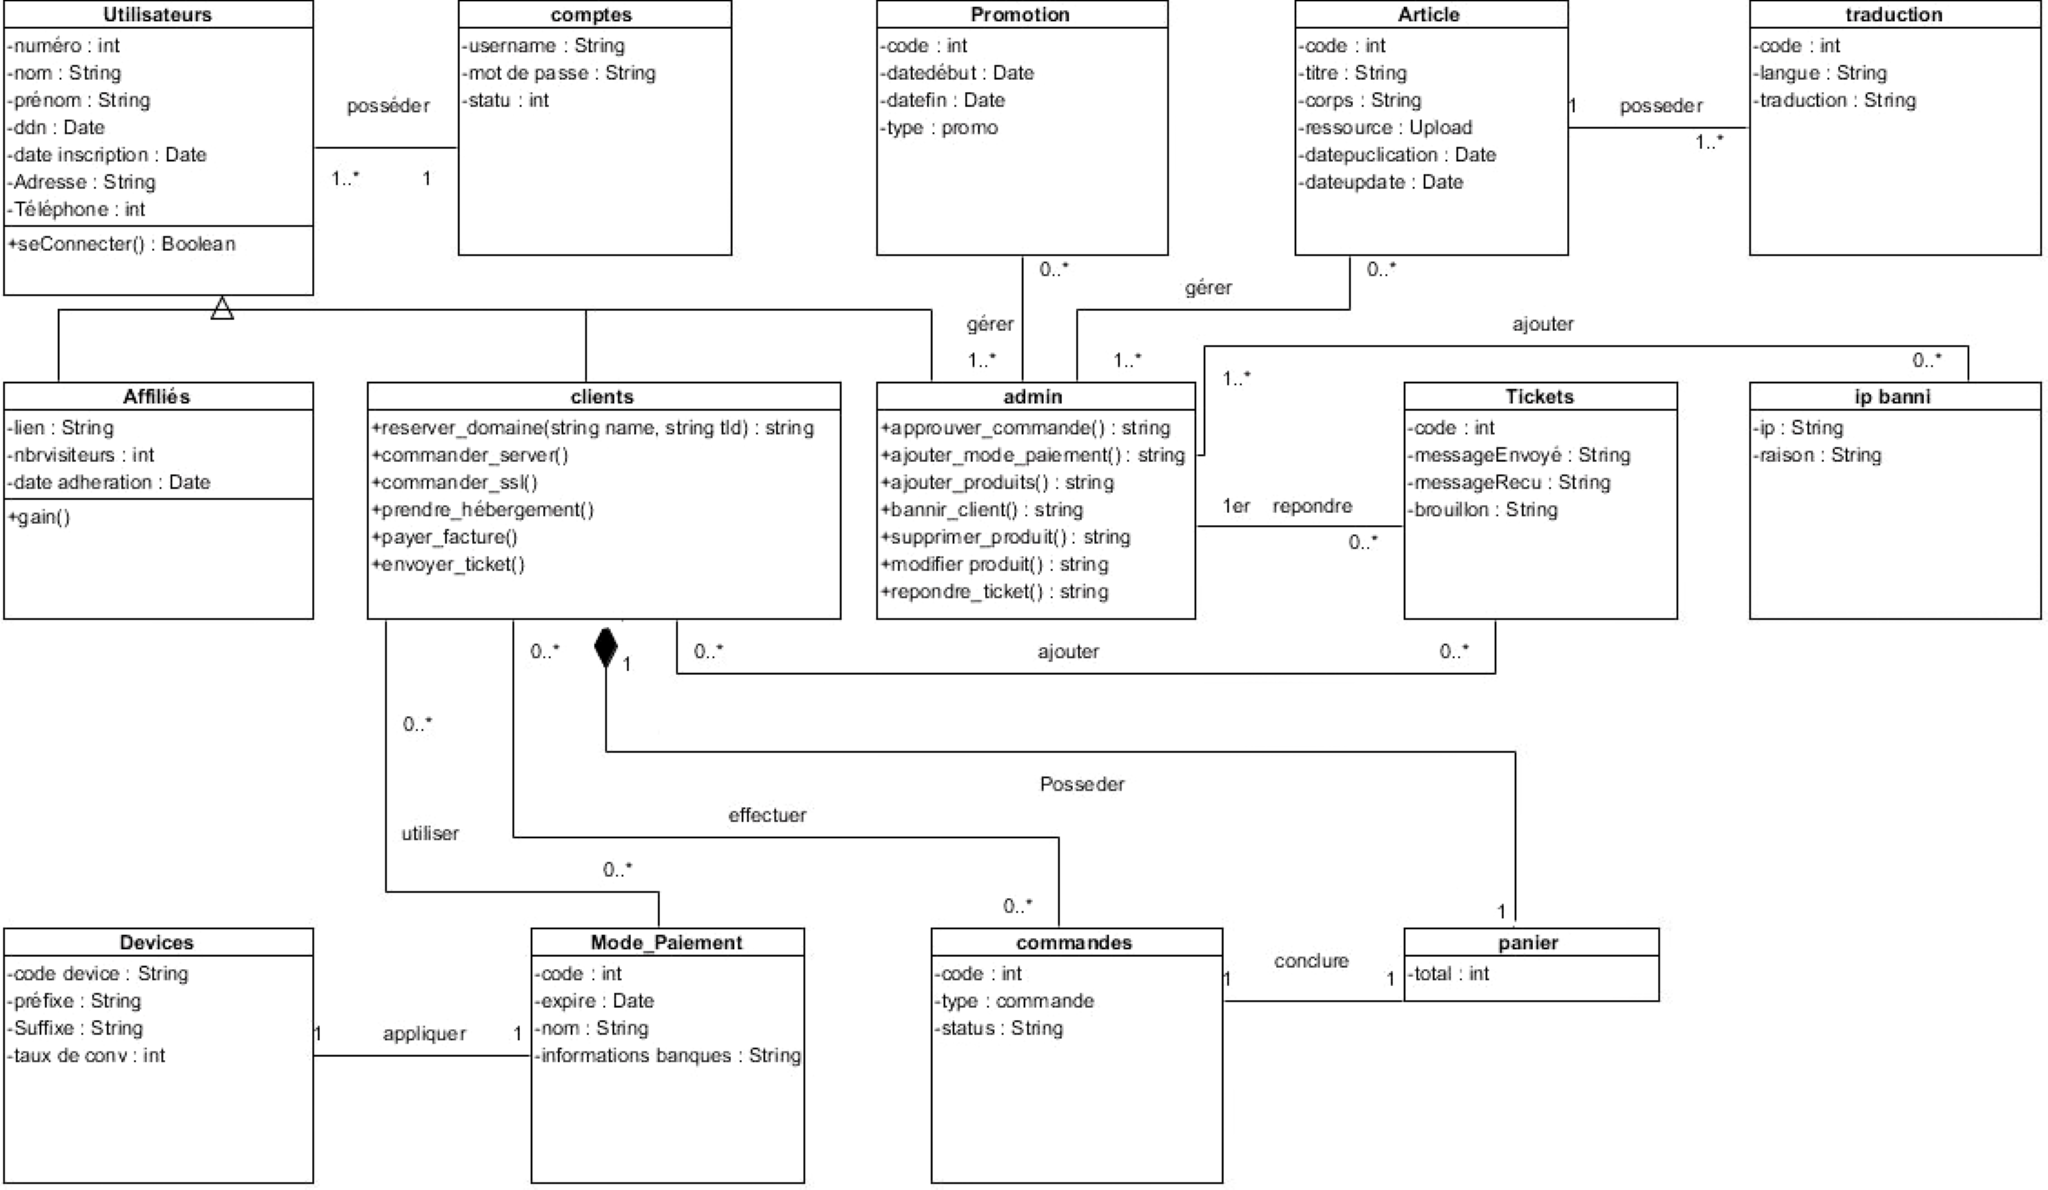
\includegraphics{img/diagclasse/3}
		\caption{Diagramme de Classe De conception (1/2)}
		\label{Tux}
	\end{figure}
	\begin{figure}[H]
	\centering
	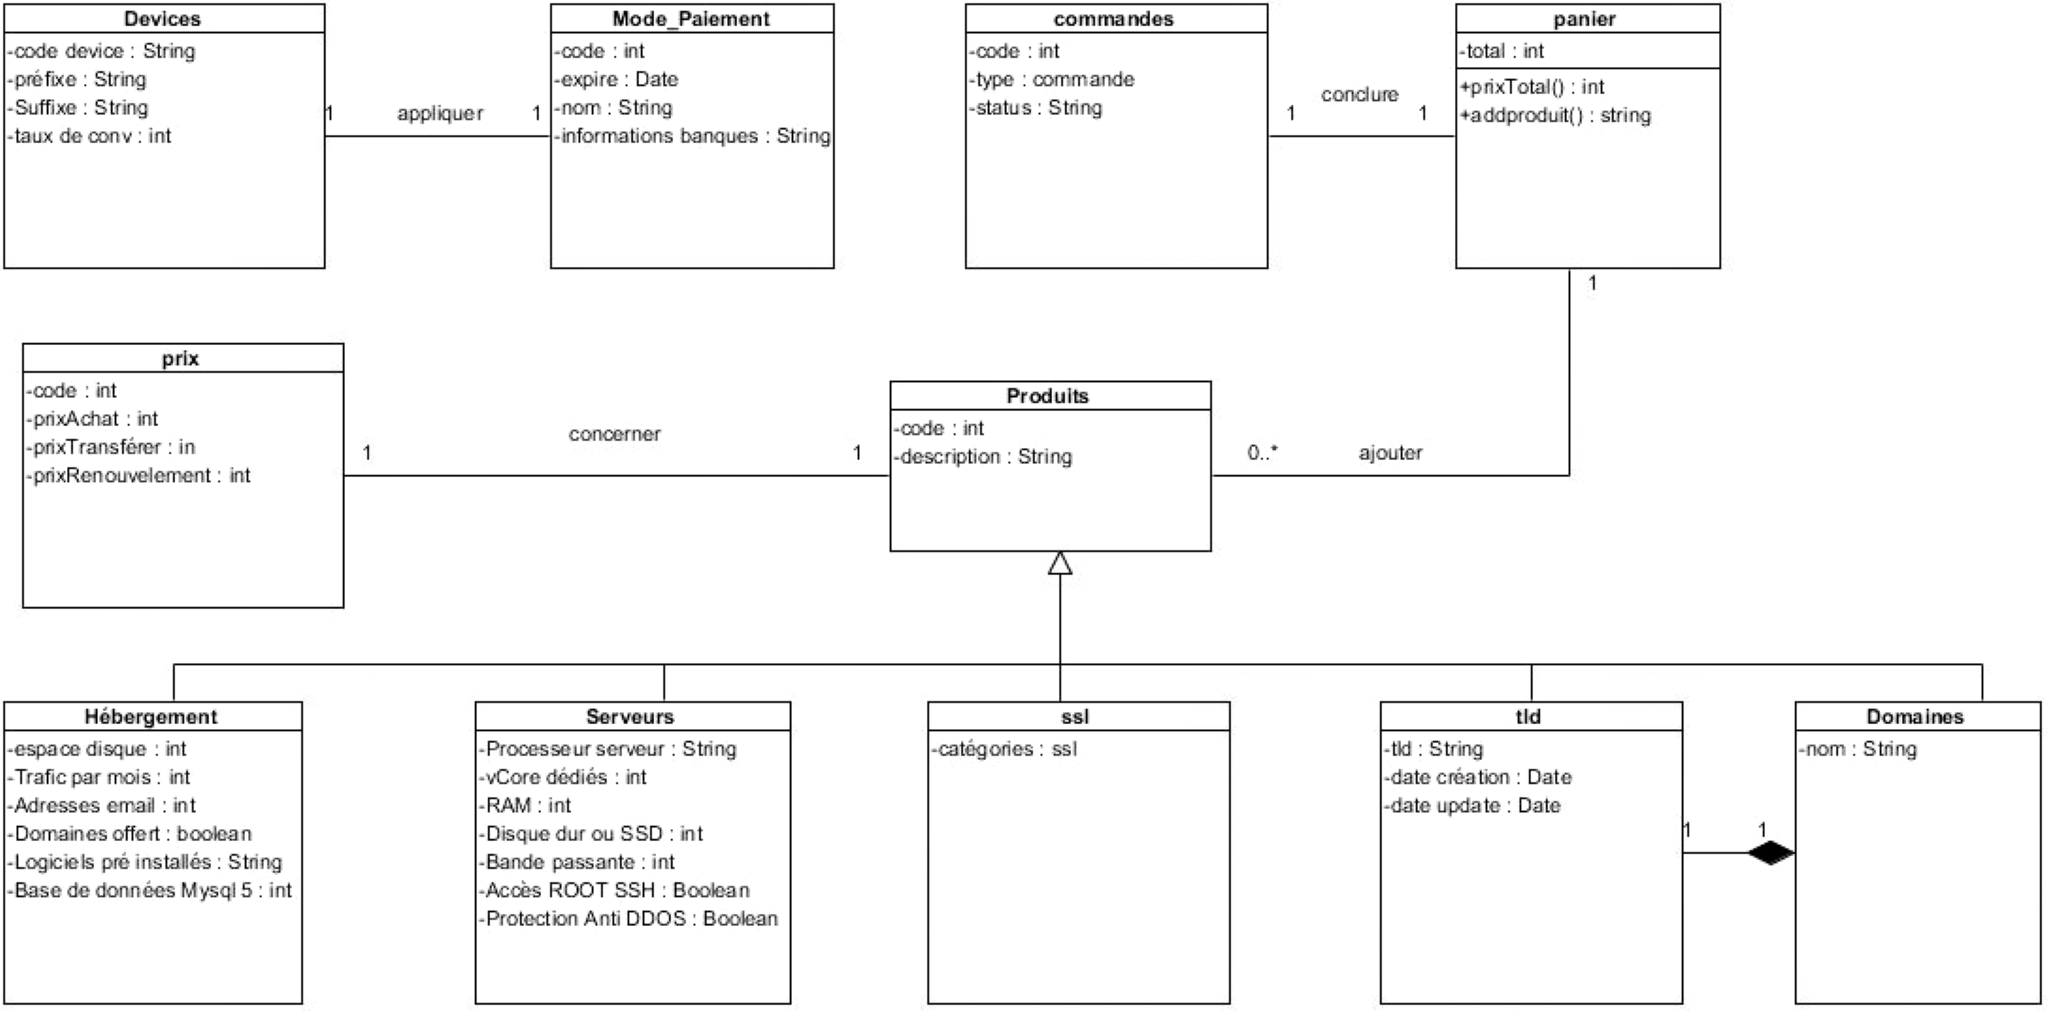
\includegraphics{img/diagclasse/4}
	\caption{Diagramme de Classe De conception (2/2)}
	\label{Tux}
\end{figure}
%CHAPITRE 3
\chapter{ Conception de la plateforme }
\textit{\textbf{Résumé:} }
\setcounter{minitocdepth}{1}
\minitoc

	\section{Architecture Logique}

\section{Choix des outils Technologique}
\subsection{Outil de modélisation UML}
\noindent $\blacktriangleright$ Visual Paradigm
\\

\includegraphics{img/outils/1}
\\
\noindent Visual Paradigm for UML est comme son nom le laisse
\\
 supposer, un logiciel permettant aux programmeurs de mettre en place des diagrammes UML. Disposant d’un outil créant des rapports personnalisables aux formats PDF, Word ou HTML afin de les partager et les publier sur Internet, cette application est compatible avec de nombreuses applications, standards et environnements. Ainsi, vous pourrez générer notamment des diagrammes de séquences ou de cas d’utilisation at ainsi de produire du code source dans de nombreux langages comme le JAVA ou encore le C++, ou bien faire l’inverse, générer des diagrammes à partir de code déjà existant
\subsection{Langage de programmation}
\noindent $\blacktriangleright$ HTML
\\

\includegraphics{img/outils/2}
\\
\noindent HTML (HyperText Markup Language/langage hypertexte) est le langage dans lequel sont écrites les pages du web. Un site Web est constitué d’un ou de plusieurs documents HTML, appelées aussi pages. Pour se déplacer d’une page à l’autre dans nos modules en passe par l’intermédiaire d’hyperliens. Pour ajouter des objets graphiques on utilise le HTML d’autre part pour tester des pages web html en local, il suffit d’ouvrir le fichier dans un navigateur. Le HTML n’est pas un langage de programmation comme le C++. Les langages dynamiques comme PHP et JavaScript vont d’ailleurs générer des pages HTML statiques.
\\
\\
\noindent $\blacktriangleright$ JavaScript
\\
\includegraphics{img/outils/3}
\\
\noindent JavaScript est un langage de programmation de scripts principalement utilisé pour les pages web interactives comme les pages HTML. JavaScript est exécuté sur l’ordinateur de l’internaute par le navigateur lui-même. C’est une extension de langage HTML qui est incluse dans le code. Ce langage est un langage de programmation qui permet d’apporter des améliorations au langage HTML en permettant d’exécuter des commandes. Ce code est directement écrit dans la page HTML, c’est un langage peu évolué qui ne permet aucune confidentialité au niveau des codes.
Dans l’application nous avons codé plusieurs fonctions. JavaScript par exemple : pour l’interaction des pages en envoyant des variables dans l’adresse URL pour filtrer le résultat de la requête en utilisant la méthode POST ou GET.
\\
\\
\noindent $\blacktriangleright$ PHP
\\
\includegraphics{img/outils/4}
\\
\noindent PHP est un langage interprété (un langage de script) exécuté du côté serveur (comme les scripts CGI, ASP, ...) et non du côté client (un script écrit en JavaScript ou une applet Java s'exécute au contraire sur l'ordinateur où se trouve le navigateur). La syntaxe du langage provient de celles du langage C, du Perl et de Java.
\\
\noindent Ses principaux atouts sont :
\\
\noindent $\bullet$ La gratuité et la disponibilité du code source (PHP est distribué sous licence GNU GPL)
\\
\noindent $\bullet$ La simplicité d'écriture de scripts
\\
\noindent $\bullet$ La possibilité d'inclure le script PHP au sein d'une page HTML (contrairement aux scripts CGI, pour lesquels il faut écrire des lignes de code pour afficher chaque ligne en langage HTML)
\\
\noindent $\bullet$ La simplicité d'interfaçage avec des bases de données (de nombreux SGBD sont supportés, le plus utilisé avec ce langage est MySQL).
\\
\noindent $\bullet$ L'intégration au sein de nombreux serveurs web (Apache...)
\\
\\
\noindent $\blacktriangleright$ CSS
\\
\includegraphics{img/outils/5}
\\
\noindent Le CSS, Cascading Style Sheets (feuilles de styles en cascade), servent à mettre en forme des documents web, type page HTML ou XML. Par l’intermédiaire de propriétés d’apparence (couleurs, bordures, polices, etc.) et de placement (largeur, hauteur, côte à côte, dessus, dessous, etc.), le rendu d’une page web peut être intégralement modifié sans aucun code supplémentaire dans la page web. Les feuilles de style ont d’ailleurs pour objectif principal de dissocier le contenu de la page de son apparence visuelle.
\subsection{Outil d’administration de la base de données}
\noindent $\blacktriangleright$ MySQL
\\
\includegraphics{img/outils/6}
\\
\noindent MySQL est un système de gestion de base de données (SGBD). MySQL est donc un programme qui permet d'enregistrer et de classer des informations dans une base de données.
\\
Il est très utilisé dans les projets libres et dans le milieu industriel. MySQL est un SGBDR facile à utiliser qui convient très bien pour la plupart des sites web.
\\
La rapidité de développement a été, depuis le début l’objectif principal de ceux qui l’ont écrit. Pour cela ils ont décidé de proposer moins de fonctionnalités, mais son installation et son utilisation sont plus aisées.
\subsection{Outil web serveur}
\noindent $\blacktriangleright$ APACHE
\\
\includegraphics{img/outils/7}
\\
\noindent Le logiciel libre Apache HTTP Server (Apache) est un serveur HTTP créé et maintenu au sein de la fondation Apache. C'est le serveur HTTP le plus populaire du World Wide Web. Il est distribué selon les termes de la licence Apache.

Apache fonctionne principalement sur les systèmes d'exploitation UNIX (Linux, Mac OS X, Solaris, BSD et UNIX) et Windows...
Apache est conçu pour prendre en charge de nombreux modules lui donnant des fonctionnalités supplémentaires : interprétation du langage Perl, PHP, Python et Ruby, serveur proxy, Common Gateway Interface, Server Side Includes, réécriture d'URL, négociation de contenu, protocoles de communication additionnels, etc. Néanmoins, il est à noter que l'existence de nombreux modules Apache complexifie la configuration du serveur web. En effet, les bonnes pratiques recommandent de ne charger que les modules utiles : de nombreuses failles de sécurité affectant uniquement les modules d'Apache sont régulièrement découvertes.
\\
\\
Les possibilités de configuration d'Apache sont une fonctionnalité phare. Le principe repose sur une hiérarchie de fichiers de configuration, qui peuvent être gérés indépendamment. Cette caractéristique est notamment utile aux hébergeurs qui peuvent ainsi servir les sites de plusieurs clients à l'aide d'un seul serveur HTTP. Pour les clients, cette fonctionnalité est rendue visible par le fichier .htaccess.
\\
\\
Parmi les outils aidant la maintenance d'Apache, les fichiers de log peuvent s'analyser à l'aide de nombreux scripts et logiciels libres tels que AWStats, Webalizer ou W3Perl. Plusieurs interfaces graphiques facilitent la configuration du serveur.
\subsection{Outil de gestions}
\noindent $\blacktriangleright$ WHMCS
\\
\includegraphics{img/outils/8}
\\
\noindent WHMCS est un outil de facturation commerciale et de gestion des clients. Initialement sorti en 2005, WHMCS a connu une croissance pour devenir la solution de facturation la plus populaire intégrée pour les fournisseurs de services d'hébergement Web.

WHMCS est une gestion de la clientèle tout-en-un, la facturation et la solution de soutien aux entreprises en ligne. Manipulation de tout, de la cessation d'inscription, WHMCS est un puissant outil d'automatisation qui vous met bien en main. Si une solution populaire pour les fournisseurs de services d'hébergement Web, WHMCS dispose également d'un nombre croissant de clients utilisant la solution à d'autres fins.
\\
\\
\noindent $\blacktriangleright$ cPanel
\\
\includegraphics{img/outils/9}
\\
\noindent CPanel, comme son nom l’indique, est un panneau de contrôle basé sur le Web utilisé pour gérer des serveurs Web ou serveurs basés sur Linux ou Windows. L’hébergement cPanel permet aux utilisateurs de contrôler les adresses e-mail, les noms de domaine, les bases de données, les différentes versions de PHP et presque tous les aspects d’un serveur Web, permettant ainsi de gérer tous les services hébergés en un seul endroit.\\
\\
\noindent $\blacktriangleright$ Virtualizor
\\
\includegraphics{img/outils/10}
\\
\noindent Virtualizor est un puissant panneau de configuration VPS basé sur le Web, qui permet à un utilisateur de déployer et de gérer VPS sur des serveurs en un seul clic. Virtualizor prend en charge les systèmes KVM, Xen, OpenVZ, Proxmox, Virtuozzo, LXC, etc. 
\subsection{Technologies de virtualisation}
\noindent $\blacktriangleright$ KVM
\\
\includegraphics{img/outils/11}
\\
\noindent KVM (Kernel-based Virtual Machine) est une technologie de virtualisation Open Source intégrée à Linux. Avec KVM, vous pouvez transformer Linux en un hyperviseur qui permet à une machine hôte d'exécuter plusieurs environnements virtuels isolés, appelés invités ou machines virtuelles.
KVM fait partie de Linux. Si vous disposez de Linux 2.6.20 ou d'une version plus récente, alors vous disposez de KVM. La technologie KVM a été présentée pour la première fois en 2006, puis intégrée à la version du noyau Linux mainline un an plus tard. Comme la technologie KVM fait partie du code Linux existant, elle bénéficie immédiatement de chaque nouvelle fonctionnalité, nouveau correctif ou nouvelle amélioration apportés à Linux sans qu'aucune intervention supplémentaire ne soit nécessaire. 
\\
\noindent $\blacktriangleright$ LXC 
\\
\includegraphics{img/outils/12}
\\
\noindent LXC, contraction de l’anglais Linux Containers est un système de virtualisation, utilisant l’isolation comme méthode de cloisonnement au niveau du système d’exploitation.
Ce système est similaire aux autres systèmes de virtualisations au niveau du système d’exploitation comme openVZ, Linux-VServer sur Linux ou comme les BSD jails de FreeBSD, ou encore les zones Solaris.
Une solution de virtualisation de type isolateur permet la virtualisation par container au niveau du noyau. LXC est très récent et remplace Linux-VServer et OpenVZ.  Aussi, LXC est dès à présent intégré au noyau, ce qui n’a jamais été le cas des deux solutions citées précédemment.
Le conteneur apporte une virtualisation de l’environnement d’exécution (Processeur, Mémoire vive, réseau, système de fichier…) et non pas de la machine. Pour cette raison, on parle de « conteneur » et non de machine virtuelle.
\\
\noindent $\blacktriangleright$ OpenVZ
\\ 
\includegraphics{img/outils/13}
\\
\noindent OpenVZ est une solution de virtualisation légère pour Linux créée en 2005.
Comme toute solution de virtualisation légère, il n'est possible d'exécuter que des systèmes Linux au sein d'OpenVZ. Cependant ce handicap est compensé par des performances bien plus proches des performances natives que tout autre type de virtualisation, en particulier pour les entrées-sorties, ainsi qu'une consommation de mémoire réduite. OpenVZ est principalement utilisé dans les environnements de développement et de tests, où il n'est pas rare d'avoir plusieurs dizaines de systèmes sur un même hôte.

\section{Architecture technique}
\section{Présentation de l’application}	
\begin{figure}[H]
	\centering
	\includegraphics{img/solution/1}
	\caption{Capture d'écran de la page d'accueil (1/4)}
	\label{Tux}
\end{figure}
\begin{figure}[H]
	\centering
	\includegraphics{img/solution/2}
	\caption{Capture d'écran de la page d'accueil (2/4)}
	\label{Tux}
\end{figure}
\begin{figure}[H]
	\centering
	\includegraphics{img/solution/3}
	\caption{Capture d'écran de la page d'accueil (3/4)}
	\label{Tux}
\end{figure}
\begin{figure}[H]
	\centering
	\includegraphics{img/solution/4}
	\caption{Capture d'écran de la page d'accueil (4/4)}
	\label{Tux}
\end{figure}
\noindent Ces premières captures présente l'interface d’accueil qui est la page principale de notre application web elle se distingue des autres pages par le fait qu'elle présente le site aux visiteurs. Elle renseigne sur le propriétaire et le contenu du site en présentant SENDNS ainsi que des détails sur les différents produits en ventes 
\begin{figure}[H]
	\centering
	\includegraphics{img/solution/5}
	\caption{Capture d'écran Authentification client}
	\label{Tux}
\end{figure}
\noindent Lorsqu’un client sera bien identifié, il pourra par la suite choisir l’une des opérations suivantes et répéter l’opération jusqu’à ce qu’il termine ses besoins. Ainsi il peut se procurer un nom de domaine, transférer un nom de domaine existant à nos serveurs, acheter un serveur dédié ou un certificat SSL, associer son nom de domaine a un hébergement web, contacter le support technique, gérer son profil
Les différents formulaires d’inscription permettent d’enregistrer notamment les informations des clients, et administrateurs
La notion de formulaire s’exprime en termes de « vue », paramétrable ou l’utilisateur remplit les champs correspondants.
Ainsi un formulaire pour réserver un nom de domaine se présente comme suit :
\begin{figure}[H]
	\centering
	\includegraphics{img/solution/6}
	\caption{Capture d'écran Commander un nom de domaine (1/6)}
	\label{Tux}
\end{figure}
\noindent Grâce à cette page ci-dessus, le client peut réserver un nom de domaine, en introduisant les informations qui lui sont relatives (nom de domaine, tld,). Après avoir saisi les informations du domaine, l’utilisateur doit valider la saisie. En cliquant sur le bouton Rechercher pour vérifier la disponibilité du nom de domaine afin de l’acquérir comme le montre l’image ci-dessous 
\begin{figure}[H]
	\centering
	\includegraphics{img/solution/7}
	\caption{Capture d'écran Commander un nom de domaine (2/6)}
	\label{Tux}
\end{figure}
\noindent On voit que notre nom de domaine est disponible d’où on peut l’acquérir. Il restera à ajouter des options supplémentaires au domaine tel qu’un hébergement web, la gestion de DNS ceci est illustré par l’image ci-dessous
\begin{figure}[H]
	\centering
	\includegraphics{img/solution/8}
	\caption{Capture d'écran Commander un nom de domaine (3/6)}
	\label{Tux}
\end{figure}
\noindent Il est possible d’appliquer un code promo définit par l’administrateur du système qui va permettre de réduire considérablement le montant total à payer
\begin{figure}[H]
	\centering
	\includegraphics{img/solution/9}
	\caption{Capture d'écran Commander un nom de domaine (4/6)}
	\label{Tux}
\end{figure}
\noindent Après avoir saisi le code promo on peut maintenant cliquer sur le bouton "passer la commande "ce pendant pour pouvoir passer une commande il faudrait au préalable être un client d’où le système va vous créer un compte client cependant si vous possédez déjà un compte il faudrait s’authentifier afin de continuer 
\begin{figure}[H]
	\centering
	\includegraphics{img/solution/10}
	\caption{Capture d'écran Commander un nom de domaine (5/6)}
	\label{Tux}
\end{figure}
\begin{figure}[H]
	\centering
	\includegraphics{img/solution/11}
	\caption{Capture d'écran Commander un nom de domaine (6/6)}
	\label{Tux}
\end{figure}
\begin{figure}[H]
	\centering
	\includegraphics{img/solution/12}
	\caption{Capture d'écran Page d’accueil client}
	\label{Tux}
\end{figure}
%CHAPITRE 4
\chapter{Plan d'affaires}
\textit{\textbf{Résumé:}}
\setcounter{minitocdepth}{2}
\minitoc
\section{Le potentiel de marché}
\noindent On dénombre actuellement plus de 600 Millions de sites web dans le monde, de plus en plus de gens ont accès à internet, les internautes passent de plus en plus de temps devant leur écran et le marché de l'internet est en plein boom. Le Net ne cesse de grossir à une vitesse démentielle : il y a eu 5,1\% de sites en plus début mars 2012 par rapport au mois précédent et fin 2011, six millions de noms de domaines supplémentaires ont été ajoutés à l'Internet.
Aucun doute, nous sommes rentrés dans l’ère internet. Les hébergeurs internet sont donc indispensables : ils stockent tous les sites web sur des ordinateurs conçus pour sauvegarder des millions de données et gérer les échanges ou flux de données.

\section{La pertinence de l’offre de valeur}
\noindent Tout type d'entreprise a besoin d'un hébergement Web professionnel fiable, un serveur rapide, et un support client sur lequel il peut compter.
Notre cœur de métier étant l’hébergement de sites web, nos clients auront à leurs dispositions des serveurs VPS, des hébergements web, des serveurs dédiés, des serveurs Cloud de qualité à moindre coût !
Pour moins de 20 000 FCFA par an, nous avons la certitude que le site du client est hébergé dans de bonnes conditions et bénéficie d’un ensemble d’outils clés en main afin de vous offrir simplicité, sécurité et performance. 
Avec SENDNS le client est certain d’avoir toujours une réponse aux questions qu’il est susceptible de se poser :
\\
\noindent $\blacktriangleright$ Utilisation de l’interface d’administration : SENDNS a mis à la disposition des clients une interface d’administration simple à prendre en main. En effet, il est possible de gérer à partir de d’une interface toutes les fonctions souhaitées : gestion des fichiers, création de boîte mail, gestion des bases de données, installation de scripts, redirection web…etc.
\\
\noindent $\blacktriangleright$ Accès SSH : SSH est devenu une référence pour sécuriser l’accès à un compte.
\\
\noindent $\blacktriangleright$ Statistiques : Nous mettons à disposition de chaque formule d’hébergement des modules de statistiques afin que le client puisse étudier les fréquences de visite et d’établir un profil type des visiteurs.
\\
\noindent $\blacktriangleright$ Compte email : le client peut créer des adresses mails de contact afin que ses visiteurs   puissent le contacter directement à partir de contact@mondomaine.com (par exemple).
\\
\noindent $\blacktriangleright$ Temps de service garanti : La satisfaction client primant avant tout, vous êtes certain d’avoir une réponse aux questions que vous vous posez.
Aide en ligne : nous mettons en ligne des vidéos, des tutoriels afin que nos clients puissent mettre en place les fonctionnalités qu’ils souhaitent sur leurs sites internet. 

\section{La capacité à s’insérer sur le marché}
Il existe aujourd'hui de nombreuses offres d'hébergement sur le marché qui sont proposées par des hébergeurs allant du simple revendeur jusqu'aux grands opérateurs Internet.
Au-delà des simples critères de prix de l'hébergement ou de notoriété du prestataire, de nombreux autres facteurs doivent être pris en compte dans le choix de votre hébergeur, surtout pour un serveur dédié.
\\
\noindent $\blacktriangleright$ Liberté
\\
La plupart des contrats de location de serveurs dédiés nécessite un engagement minimum de 12 mois voire plus, ce n'est pas le cas de SENDNS qui vous laisse une totale liberté. Tous nos contrats sont sous forme d'abonnement mensuel, sans engagement minimum de durée. Vous pouvez donc à tout moment décider d'interrompre votre abonnement. Pour des sites événementiels, vous pouvez ainsi envisager de louer un serveur pour 3 mois ou même seulement 1 mois. 
\\
\noindent $\blacktriangleright$ Flexibilité
\\
Le client est libre de changer d'offre à tout moment afin d'adapter une solution d'hébergement adaptée à ses besoins. SENDNS peut upgrader un serveur ou d'assurer la migration des données sur un autre serveur.
\\
\noindent $\blacktriangleright$ Disponibilité \& Réactivité
\\
Assurer un réel service client est notre priorité. Le support technique est joignable par mail ou par téléphone. En dehors des heures de bureau le client contacter directement les administrateurs systèmes d'astreinte qui interviennent 7J/7 et 24H24 pour les problèmes urgents. 
\\
\noindent $\blacktriangleright$ Sécurité \& Performance
\\
Tentative d'intrusion, déni de service... la sécurité des serveurs et des données est un enjeu majeur qui est malheureusement souvent négligé. Alors que beaucoup de prestataires se contentent de proposer des serveurs avec une distribution Linux par défaut, SENDNS propose 
une distribution Linux optimisée par nos ingénieurs, plus performante et surtout beaucoup plus sûr dans le cadre d'une activité d'hébergement. Cette configuration, qui a notamment fait l'objet d'audits de sécurité, est installée par défaut sur tous nos serveurs Linux. 
\\
\noindent $\blacktriangleright$ Simplicité 
\\
Administrer un serveur a longtemps été réservé à des spécialistes, mais ce n'est plus le cas aujourd'hui. Pour les serveurs Linux, SENDNS propose une interface Web d'administration exclusive permettant de réaliser en quelques clics toutes les opérations courantes : création de comptes Web et FTP, de comptes mail, de DNS... 
\\
\noindent $\blacktriangleright$ Compétitivité
\\
Avec des forfaits tout compris incluant à la fois le serveur, une connexion haut débit et de nombreux services, nos offres sont parmi les plus compétitives du marché. De plus nos contrats sont sans surprise, pas d'options cachées ou de facturation de dépassement de trafic. Notre meilleure garantie est notre contrat sans engagement, ainsi le client est libre d'interrompre le contrat à tout moment s’il n’est pas satisfait de nos services.
\section{Un bon retour sur investissement}	
\begin{figure}[H]
	\centering
	\includegraphics{img/bp}
	\caption{Capture d'écran Plan d'affaires}
	\label{Tux}
\end{figure}

\chapter*{Conclusion et Perspectives} \mtcaddchapter
\markboth{Conclusion et Perspectives}{}
\addcontentsline{toc}{chapter}{Conclusion et Perspectives}
\noindent Le présent rapport est le résultat du travail effectué dans le cadre du stage de fin d’étude pour l’obtention du diplôme d’ingénieur en conception. À travers ce stage, j’ai pu mettre en pratique les connaissances théoriques et pratique acquises durant ma formation, de plus, je suis arrivée a réalisé les objectifs évoqués au début. J’ai pu mettre en place un registraire qui permet aux entreprises de pouvoir se procurer facilement un site internet, de pouvoir acheter tous les dispositifs nécessaires pour avoir un site web puissant, rapide et sécurisé je fais références au différent produit vendu à travers le site il s’agit des serveurs, des certificats SSL etc.
De ce qui précède, il est difficile de prétendre avoir eu une solution idéale, toutefois j’espère avoir répondu tant soi peu au problématique et confirmé les hypothèses et dans ce qui suit nous vais essayer de lister des perspectives du système. Autrement dit, je vais présenter les améliorations qui peuvent y être apportées.
Partie technique :
\\
\noindent $\blacktriangleright$ Référencer le site web au niveau des moteurs de recherche (google et bing)                                                                               afin d’être visible à travers des mots clés
\\ 
\noindent $\blacktriangleright$ Avoir notre propre Datacenter ici à Dakar.
\bibliographystyle{plain}
\bibliography{biblio}

\chapter*{Annexes} \mtcaddchapter
\addcontentsline{toc}{chapter}{Annexes}
\markboth{Annexes}{}
\newpage


\section*{Résumé \markboth{}{}}
\thispagestyle{empty}


\section*{Abstract \markboth{}{}} 

\end{document}
